\documentclass[pra,
aps,
twocolumn,
superscriptaddress,
groupedaddress,
nofootinbib,
reprint
]{revtex4-1}

% PACKAGES
\usepackage{amsmath,amsfonts, amssymb, amsthm}
\usepackage{bm, bbm, physics, mathtools}
\usepackage{graphicx, subfigure}
\usepackage{xcolor, enumerate}
\usepackage{xifthen, hyperref}
\usepackage[capitalise]{cleveref}

\hypersetup{
	colorlinks=true,  
	linkcolor=blue,   
	citecolor=blue,   
	urlcolor=blue     
}

\newcommand{\crefrangeconjunction}{--}
\creflabelformat{figure}{(#2#1#3)}

% COMMENT NOTATION
\newcommand{\nick}[1]{{\color{red}#1}}
\newcommand{\ddd}[1]{\textcolor{blue}{#1}}

% ENVIRONMENTS
\newtheorem{theorem}{Theorem}
\newtheorem{proposition}[theorem]{Proposition}
\newtheorem{lemma}[theorem]{Lemma}
\newtheorem{definition}[theorem]{Definition}

% REFERENCES
\iffalse
\renewcommand{\eqref}[1]{Eq.~(\ref{#1})}
\newcommand{\figref}[1]{Fig.~(\ref{#1})}
\newcommand{\tabref}[1]{Tab.~(\ref{#1})}
\newcommand{\secref}[1]{Section~(\ref{#1})}
\newcommand{\appref}[1]{Appendix~(\ref{#1})}
\newcommand{\defref}[1]{Definition~\ref{#1}}
\newcommand{\lemref}[1]{Lemma~\ref{#1}}
\newcommand{\thmref}[1]{Theorem~\ref{#1}}
\fi

% SYMBOL DEFINITIONS
\renewcommand{\cal}[1]{\mathcal{#1}}

\newcommand{\reals}{\mathbb{R}}
\newcommand{\id}{\mathbbm{1}}
\newcommand{\idc}{1_{\rm{C}}}
\newcommand{\supf}{\mathfrak{c}}
\renewcommand{\tr}{{\rm{tr}}}
\renewcommand{\det}{{\rm{det}}}
\newcommand{\floor}[1]{\left\lfloor #1 \right\rfloor}
\newcommand{\ent}[2]{S\left( #1 \middle\vert\middle\vert #2 \right)}
\newcommand{\ents}{{\ent{\frac{m}{n}}{p}}}

\def\dummy{\ell}
\def\NN{n}
\def\mmf{i}
\def\nnf{n}
\def\mlt{m}
\def\ii{i}
\def\jj{j}
\def\kk{k}
\def\II{I}
\def\nn{n}
\def\tt{n'}
\def\mm{a}
\def\wp{u}
\def\wn{v}

\newcommand{\too}[1]{^{\otimes #1}}
\newcommand{\noisys}{\rho_{\rm{S}}}
\newcommand{\noisysn}{\rho_{\rm{S}}(\epsilon)^{\otimes \nn}}
\newcommand{\noisysN}{\rho_{\rm{S}}(\epsilon)^{\otimes \NN}}

\newcommand{\spanv}[1]{
    {{\rm{span}}\left\{#1\right\}}
}
\newcommand{\conv}[1]{
    {{\rm{conv}}#1}
}
\newcommand{\orb}[1]{
    {{\rm{orb}}(#1)}
}
\newcommand{\sn}[1]{
    {{\rm{sn}}\left(#1\right)}
}
\newcommand{\mana}[1]{
    {{\rm{mana}}\left(#1\right)}
}
\newcommand{\lc}[2]{
	{{\rm{L}}_{#1|#2}}
}

\newcommand{\bmx}{\bm{x}}
\newcommand{\bmy}{\bm{y}}
\newcommand{\bmz}{\bm{z}}
\newcommand{\bmu}{\bm{u}}
\newcommand{\bmw}{\bm{w}}
\newcommand{\bmo}{\bm{0}}
\newcommand{\bmd}{\bm{d}}
\newcommand{\bma}{\bm{a}}
\newcommand{\bmxi}{\bm{\xi}}
\newcommand{\bmg}{\bm{g}}

\newcommand{\zd}[1][]{
    \ifthenelse{\isempty{#1}}{
    {\mathbb{Z}_d} }{
    {\mathbb{Z}_{#1}}}
}
\newcommand{\hd}[1][]{
    \ifthenelse{\isempty{#1}}{
    {\cal{H}_d} }{
    {\cal{H}_{#1}}}
}
\newcommand{\pd}[1][]{
    \ifthenelse{\isempty{#1}}{
    {\cal{P}_d} }{
    {\cal{P}_{#1}}}
}
\newcommand{\cd}[1][]{
    \ifthenelse{\isempty{#1}}{
    {\cal{C}_d} }{
    {\cal{C}_{#1}}}
}
\newcommand{\spd}[1][]{
    \ifthenelse{\isempty{#1}}{
    {{\rm{Sp}}(2, \zd)} }{
    {{\rm{Sp}}(2, \zd[#1])}}
}
\newcommand{\gp}[1][]{
    \ifthenelse{\isempty{#1}}{
    {\rm{GP}_d} }{
    {\rm{GP}_{#1}}}
}
\newcommand{\stoch}[1][]{
    \ifthenelse{\isempty{#1}}{
    {{\rm{S}}_d(\bmd)} }{
    {{\rm{S}}_d(#1)}}
}
\newcommand{\stochw}[1][]{
    \ifthenelse{\isempty{#1}}{
    {{\rm{S}}_{d^2}(\W{\sigma})} }{
    {{\rm{S}}_{d^2}(#1)}}
}
\makeatletter
\def\W{\@ifnextchar[{\@with}{\@without}}
\def\@with[#1]#2{ 
    {{\rm{W}}_{#2}\left(#1\right)} }
\def\@without#1{ 
    {{\rm{W}}_{#1}} }
\makeatother

\newcommand{\T}{\cal{T}}
\newcommand{\Z}{\cal{Z}}

\newcommand{\C}{\cal{C}}
\newcommand{\E}{\cal{E}}
\newcommand{\J}{\cal{J}}
\newcommand{\R}{\cal{R}}
\newcommand{\D}{\cal{D}}
\newcommand{\F}{\cal{F}}
\renewcommand{\O}{\cal{O}}
\newcommand{\M}{\cal{M}}

\newcommand{\Fmax}{\F_{\rm{max}}}
\newcommand{\Omax}{\O_{\rm{}max}}
\newcommand{\Rmax}{\R_{\rm{}max}}
\newcommand{\Pis}{\Pi_{\rm{s}}}
\newcommand{\Pio}{\Pi_{\rm{o}}}

\newcommand{\cptp}{{\rm{CPTP}}}
\newcommand{\cpos}{{\rm{CP}}}
\newcommand{\so}{{\rm{SO}}}
\newcommand{\stab}{{\rm{STAB}}}
\newcommand{\spo}{{\rm{SPO}}}
\newcommand{\cspo}{{\rm{CSPO}}}
\newcommand{\rcu}{{\rm{RCU}}}
\newcommand{\tho}{{\rm{TO}}}
\newcommand{\cpwp}{{\rm{CPWPO}}}
\newcommand{\ru}{{\rm{RU}}}


\begin{document}
% Labels and Refs (consistency, cref vs ref, thm vs lem vs prop, ??)
% Figs check(fig.0, move to app, consistency)

% Notation consistency (R is rate not bound, noise vs error, \ln{} -> \ln, italics, keep \bmx for vectors?)
% UK vs US english
% Spacing (figs, sections, paragraphs, eq. numbering, \noindent, QEDs)

\begin{abstract}
\ddd{[To be sharpened]} Magic states are key ingredients in schemes to realise universal fault-tolerant quantum computation.
Theories of magic states attempt to quantify this computational element via monotones and determine how these states may be efficiently transformed into useful forms. Here we introduce the concept of `fragments', which generalise the concept of magic monotones and has a natural thermodynamic structure based on majorisation. From this perspective magic can be viewed as a form of free energy within each fragment and is constrained by relative majorisation relations but now on quasi-probability distributions. Notably this approach allows us to incorporate actual physical constraints, for example noise models with particular bias or temperature-dependent features, and study how these constrain general magic distillation protocols. In this context we present general temperature-dependent bounds on distillation rates that any theory of magic must respect. Significantly, this analysis also presents a thermodynamic context which cannot be analysed via traditional methods based on thermodynamic entropies, due to the presence of negativity, and raises novel questions in the context of statistical mechanics.
\end{abstract}

\preprint{APS/123-QED}

\title{General constraints on magic distillation protocols from statistical mechanics}

\author{Nikolaos Koukoulekidis}
	\email{nk2314@imperial.ac.uk}
	\affiliation{Department of Physics, Imperial College London, London SW7 2AZ, UK}
\author{David Jennings}
	\affiliation{School of Physics and Astronomy, University of Leeds, Leeds, LS2 9JT, UK}
	\affiliation{Department of Physics, Imperial College London, London SW7 2AZ, UK}

\date{\today}
\maketitle

%%%%%%%%%%%%%%%%%%%%%%%%%%%%%%%%%%%%%%%%

\section{Introduction}
\label{sec:intro}

\nick{Bunch of refs:}~\cite{White_2021, Rethinasamy_2020, Blackwell_1953, Sarkar_2020, Gour_2020}

The past few years have seen rapid progress towards the goal of a fault-tolerant quantum computer~\cite{Nickerson_2014, Nikahd_2017, chao_2018, lin_pieceable_2020, Lin_2020, Bourassa_2021}. However, many challenges remain and there is increasing need for theory to take into account physical limitations of the hardware involved. The surface code~\cite{Bravyi_1998, Freedman_2001, Dennis_2002, Raussendorf_2007} is a leading framework for fault-tolerance with very high error thresholds. Within this scheme, Clifford unitaries can be implemented in a robust, fault-tolerant way. However, due to the Eastin-Knill theorem~\cite{Eastin_2009}, we also know that it is impossible to have a universal set of transversal gates, and although Clifford unitaries can be realised transversally~\cite{Calderbank_1996, Steane_1996}, one needs to find ways around the Eastin-Knill restriction. This can be achieved by injecting in quantum states, called magic states, which promote the Clifford group to universal quantum computing~\cite{cit:bravyi}. The obstacle to this is that these states are invariably noisy and so protocols involving stabilizer operations must be employed to purify many copies of the magic states and improve the overall performance of the induced quantum gates. A central question then arises about the overhead on purifying many copies of a magic state into less noisy forms. 

To address this, concrete distillation protocols have been developed, such as the Bravyi-Haah protocol that provides a quadratic reduction in noise per cycle~\cite{Bravyi2012}. Such distillation rates have been improved in more recent works~\cite{Hastings2018, Litinski_2019, Krishna2019, cit:prakash}. There is also analysis of magic protocols from the perspective of magic monotones, which provide upper bounds on distillation rates and find application in the analysis of gate synthesis~\cite{Campbell_2017, Howard_2017, Prakash_2018}. These frameworks for magic view magic states as resource states with respect to a natural class of quantum operations that are considered cheap, or free, such as stabilizer operations~\cite{Gour_2019, cit:ahmadi, cit:seddon, Wang_2019}.
  
  
Recent work towards fault-tolerance has begun to bridge the gap between abstract theory and experiment. Extensive work has been done on error mitigation~\cite{Li_2017, Temme_2017, Endo_2018, McClean_2017}, and the incorporation of hardware physics into the theoretical modes~\cite{Kandala_2019, Colless_2018, song2018quantum, Bravyi_2021}. For example, the XZZX code~\cite{bonilla_ataides_xzzx_2021} is a variant of the surface code that incorporates noise bias explicitly and has been shown to attain the hashing bound of random codes~\cite{Bennett_1996}. 

In this work, we develop a framework to analyse magic state distillation protocols where explicit physics of the system is incorporated.  Distillation bounds are obtained by considering how a given magic state protocol would behave if it were instead applied to a \emph{stabilizer} state that is distinguished by the physics of the system -- for example an equilibrium state at a characteristic temperature, or the maximally mixed state. The magic distillation bounds can then be expressed in terms of this distinguished degrees of freedom (e.g. free energy changes in the case of temperature, or non-unitality in the case of the maximally mixed state). Such bounds are therefore of interest in assessing how physical features such as temperature, noise-biases or fixed-point structure associated with restricted gate-sets constrain distillation protocols, and so are of relevance to existing work towards fault-tolerant quantum computing~\cite{Aliferis_2008, Stephens_2013, Li_2015, Babbush_2018, Tuckett_2019, Guillaud_2019, Fowler_2019}. 

The approach we take is most closely aligned with resource theories of magic, however it differs in a few ways. Firstly, we obtain distillation upper bounds without the use of monotones, and secondly our distillation bounds are hardware dependent. We approach this problem using tools from statistical mechanics and recent work from the overlap of thermodynamics and quantum information theory~\cite{cit:janzing, cit:horodecki2, Brandao_2015, Vinjanampathy_2016, Goold_2016, cit:lostaglio, cit:gour}. In particular, we shall view \emph{magic as a form of free energy}, relative to the set of stabilizer states. From this perspective, the convex set of stabilizer states behaves as the set of ``equilibrium'' states, and magic corresponds to a form of non-equilibrium free energy that is strictly non-classical.

Our analysis relies on the discrete Wigner representation of quantum systems, in which all states and operations can be described on a discrete phase space~\cite{Ferrie_2008, Okay_2021}. Crucially, we focus on magic states with negativity in their Wigner representation, which is known to be a necessary condition for universality in the state-injection model~\cite{cit:veitch, cit:mari, cit:gottesman, cit:knill, Campbell_2011}. Interestingly, taking a statistical mechanical perspective in this context raises a problem, namely it is impossible to define entropies for quasi-distributions. We circumvent this obstacle by making use of a more fundamental tool in thermodynamics and information theory -- majorization theory~\cite{cit:marshall, Veinott_1971, Ruch_1976}. To our knowledge majorization of quasi-distributions has not been considered in quantum physics before, and therefore our analysis is also of interest to the study of non-classicality in quantum systems.

Through this approach we obtain a range of upper bounds for magic distillation rates. We provide explicit bounds for magic protocols that generate unital channels, as well as bounds that depend on the temperature and Hamiltonian of the system. We find that the thermodynamic ordering in the presence of negativity is non-trivial and displays a range of features that, unsurprisingly, do not appear in classical statistical mechanics. 
Finally, we discuss how our approach could be improved and how it can be exploited to construct explicit lower bounds on distillation that take into account physical structure.

\begin{figure}[t]
    \centering
        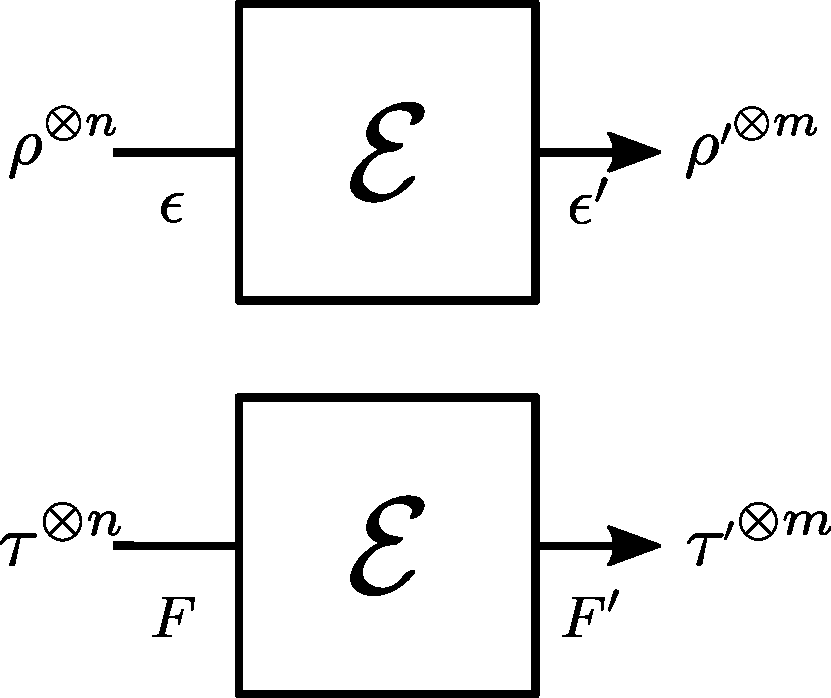
\includegraphics[scale=0.3]{figs/protocol_diagram.pdf}
    \caption{\textbf{Magic distillation protocols \& stabilizer reference states.} 
	A magic protocol (top figure) converts $n$ copies of some noisy magic state $\rho$ with noise parameter $\epsilon$ to $m$ copies of some less noisy state $\rho'$ with $\epsilon' < \epsilon$. The physics of the protocol can be analysed by considering how it would transform some distinguished reference stabilizer state $\tau^{\otimes n}$ (bottom figure). For the case where this reference state is a thermal state at some temperature $T$ our magic distillation bounds are functions of $T$, the noise parameters $\epsilon, \epsilon'$, and the free energy the protocol channel $\E$ injects in. In addition a quantity $\phi$ links the computational and physical aspects, and corresponds to the degree to which Wigner negativity in $\rho$ can be assigned a sharp energy via the system Hamiltonian.}
    \label{fig:sketch}
\end{figure}

\section{Phase space representations of quantum states}
\label{sec:ps}

Central to our construction is the representation of any quantum state or quantum operation on a system of dimension $d$ in terms of quasi-probability representations on a discrete phase space~\cite{Ferrie_2008}. This construction is a discrete version of Wigner representations in quantum optics~\cite{Wigner_1932, Vourdas_2004}.

Consider a $d$--dimensional quantum system with Hilbert space $\H_d$, and let $\{ |0\>, |1\>, \dots , |d-1\>\}$ denote the standard computational basis, defined over $\mathbb{Z}_d = \{ 0, 1, \dots,d-1 \}$. On this space, generalised Pauli matrices $X, Z$ can be defined by their respective roles as shift and phase operators, acting on the basis states as follows,
\begin{align}
    X \ket{k} &= \ket{k + 1} \label{eq:xpauli}\\
	Z \ket{k} &= \omega^k \ket{k}. \label{eq:zpauli}
\end{align}
Here $\omega \coloneqq e^{2\pi i/d}$ is the $d$-th root of unity and addition is taken modulo $d$. From these we can construct a phase space $\cal{P}_d = \mathbb{Z}_d \times \mathbb{Z}_d$ that provides a complete representation of the quantum system. Given a point $\bmx \coloneqq (x, p)$ we define a displacement operator, 
\begin{equation}\label{eq:ddef}
    D_{\bmx} \coloneqq \tau^{x p} X^{x} Z^{p},\ 
\end{equation}
where the phase factor $\tau \coloneqq -\omega^{1/2}$ ensures unitarity. We assume going forward that $d$ is an odd prime, however the case $d=2$ can also be handled, but with some additional technical caveats~\cite{Appleby_2005}. For a composite system with composite dimension $d = d_1 \dots d_n$ we can decompose the Hilbert space as $\cal{H}_d = \cal{H}_{d_1} \otimes \dots \otimes \cal{H}_{d_n}$, and then define displacement operators as
\begin{equation}\label{eq:composited}
    D_{\bmx} \coloneqq D_{(x_1, p_1)} \otimes \dots \otimes D_{(x_n, p_n)},
\end{equation}
where now we have
\begin{align*}
	\bmx \coloneqq (x_1, p_1, x_2, p_2, \dots, x_n, p_n) \in \cal{P}_{d_1} \times \dots \times \cal{P}_{d_n} \eqqcolon  \cal{P}_d,
\end{align*}
to denote the phase space point for the composite system. 
For simplicity going forward, we assume $n$ copies of a $d$--dimensional system $d_1=d_2 = \cdots = d$, and therefore we have that $\x \in \mathbb{Z}_d^{2n}$.


The displacement operators form the Heisenberg-Weyl group~\cite{Folland_1989, Bengtsson_2006} under matrix multiplication modulo phases,
\begin{equation}\label{eq:gp}
    {\rm{HW}}_d^n \coloneqq \{ \tau^k D_{\bmx}: k \in \mathbb{Z}_d, \bmx \in \cal{P}_d^n\}.
\end{equation}
The Clifford operations $ \cal{C}_d^n $ are then defined as the set of unitaries that normalise the Heisenberg-Weyl group~\cite{Appleby_2005}. We may define the pure stabiliser states as those states obtained by acting on $|0\>$ with Clifford unitaries~\cite{cit:gross3} and, finally, the full set of stabilizer states as the convex hull of all pure stabilisers, namely all probabilistic mixtures of states of the form $U|0\>\<0|U^\dagger$ where $U$ is Clifford. 

\subsection{Wigner representations for quantum states and quantum operations}\label{sec:wigner}

In order to provide a complete decomposition of arbitrary quantum states and quantum operations we now define a complete basis of Hermitian observables that behaves naturally under the action of the Clifford group. At every point $\x \in \P_d$ we define the phase-point operator
\begin{equation}\label{eq:ax}
	A_{\bmx} \coloneqq \frac{1}{d} \sum_{\bmz \in \cal{P}_d} \omega^{\eta(\bmx, \bmz)} D_{\bmz}, 
\end{equation}
where $\eta(\bmx, \bmz)$ is the symplectic inner product between any two points $\x,\z \in \P_d$, and is given explicitly by
\begin{equation}
	\eta(\bmx, \bmz) \coloneqq \bmz^T \begin{pmatrix}
		0  & \id \\ %\mathbbm{O}_n  & \id_n \\
		-\id & 0 \\ %-\id_n & \mathbbm{O}_n \\
	\end{pmatrix} \bmx,
\end{equation}
where $0, \id$ denote the $n\times n$ zero and identity matrices.

The phase-point operators form an orthogonal operator basis with respect to the Hilbert-Schmidt inner product, as discussed in~\cref{app:wigner}.
Therefore, any quantum state $\rho \in \cal{B}(\cal{H}_d)$ can be expressed as a linear combination of them,
\begin{equation}
    \rho = \sum_{\bmz \in \cal{P}_d} \W[\bmz]{\rho} A_{\bmz},
\end{equation}
where the coefficient vector $\W{\rho}$ is the Wigner distribution of state $\rho$,
\begin{equation}\label{eq:wstate}
    \W[\bmx]{\rho} \coloneqq \frac{1}{d}\tr[A_{\bmx} \rho].
\end{equation}

For any quantum state $\rho$, the Wigner distribution $W_\rho(\bmx)$ is readily seen to be a $d^2$-dimensional quasi-probability distribution over $\cal{P}_d$. More precisely, $W_\rho(\x)$ is a bounded real-valued function on $\P_d$ with the normalisation property $\sum_{\x} W_\rho(\bmx) = 1$ (see~\cref{app:wigner} for details).  In~\cref{fig:wstate_examples}, we show Wigner distributions of different types of qutrit states.

\begin{figure}[t]
    \centering
    \subfigure[][]{%
    \label{fig:maxmix}%
    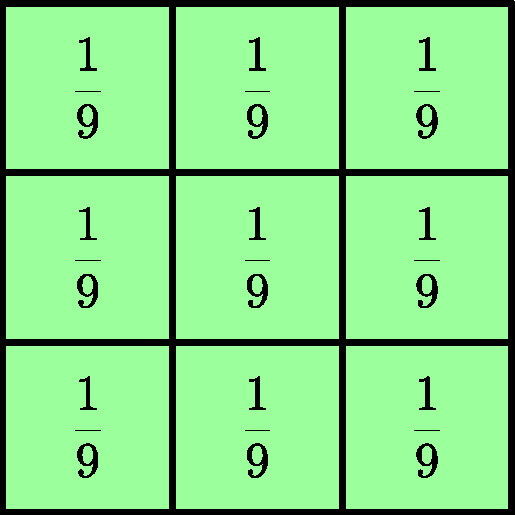
\includegraphics[height=2cm]{figs/maxmixed.pdf}
    }\hspace{8pt}%
    \subfigure[][]{%
    \label{fig:zero}%
    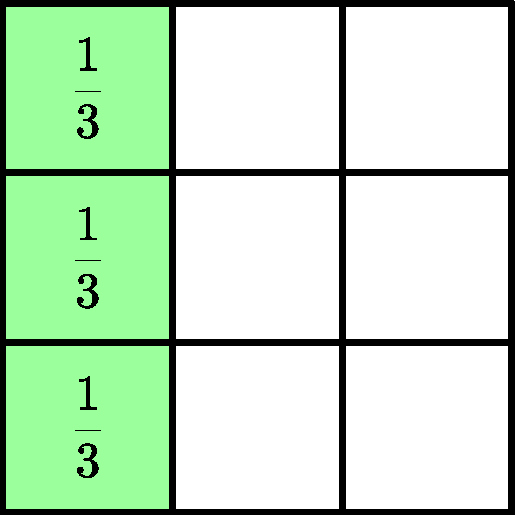
\includegraphics[height=2cm]{figs/zerostate.pdf}
    }\\
    \subfigure[][]{%
    \label{fig:bound}%
    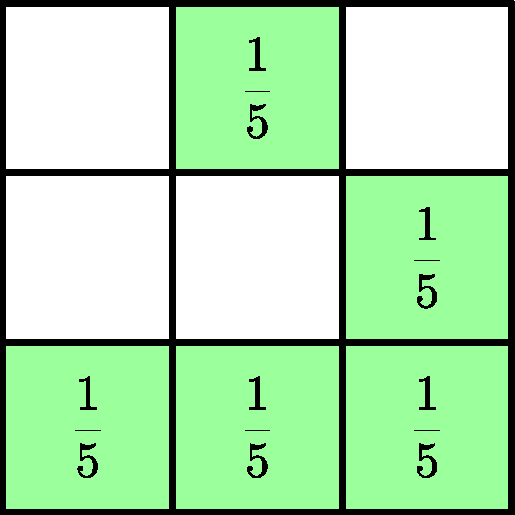
\includegraphics[height=2cm]{figs/boundstate.pdf}
    }\hspace{8pt}%
    \subfigure[][]{%
    \label{fig:Strange}%
    \includegraphics[height=2cm]{figs/Strangestate.pdf}
    }
    \caption{\textbf{Qutrit Wigner distributions of varying magic.} 
    \subref{fig:maxmix} Maximally mixed state $\frac{1}{3}\id$; \subref{fig:zero} Stabilizer zero state $|0\>\<0|$; \subref{fig:bound} A non-stabiliser Wigner-positive state; \subref{fig:Strange} Magic Strange state $\ket{{\rm{S}}} = \frac{1}{\sqrt{2}}(\ket{1} - \ket{2})$, coined in~\cite{cit:veitch2}.
    }%
    \label{fig:wstate_examples}
\end{figure}

Any quantum operation $\E$ can also admit a Wigner representation. If $\E$ maps some quantum system $A$ to a quantum system $B$, and $\J(\E)$ is its associated Choi state then we can define
\begin{equation}
W_{\E}(\y |\x) \coloneqq d_A^2 W_{\J(\E)}(\bar{\x} \oplus \y),
\end{equation}
where $\bar{x} =(x_1, -p_1, \dots , x_n, -p_n)$ can be viewed as the time-reversed version of $\x$ in the discrete phase space, where momenta are reflected while position coordinates remain unchanged.

\subsection{Magic theories for quantum computation}
\label{sec:mono}

A number of magic theories exist, with the central approach of viewing magic states as computational resource states with respect to a natural class of quantum operations that are considered free~\cite{Gour_2019}. One very natural class of free operations are those obtained from Clifford operations, measurements and the ability to discard quantum systems. However, there are also other noteworthy candidates~\cite{cit:ahmadi, cit:seddon, Wang_2019}.

In any theory of magic, a natural route to bounding the distillation rates obtainable is through the concept of a \emph{magic monotone}. A magic monotone is a real-valued function of any quantum state $\M(\rho)$ that is monotonically non-increasing under the free operations of the magic theory. More precisely $\M(\sigma) \le \M(\rho)$ whenever it is possible to convert $\rho$ into $\sigma$ using free operations (e.g. Clifford operations).

One prominent magic monotone is the \emph{mana} of a state~\cite{cit:veitch2}, defined as
\begin{equation}
    \mana{\rho} \coloneqq \ln (2\hspace{1pt}\sn{\rho}+1),
\end{equation}
where the \emph{sum-negativity}~\cite{cit:veitch2} is the sum of the negative components in $\W{\rho}$,
\begin{equation}
    \sn{\rho} \coloneqq \sum\limits_{\bmx: \W[\bmx]{\rho} < 0} \abs{\W[\bmx]{\rho}}.
\end{equation}

Mana is an additive\footnote{It satisfies the condition $\mana{\rho_1 \otimes \rho_2} = \mana{\rho_1} + \mana{\rho_2}$.} magic monotone, and the fact that it is non-increasing under free operations provides a constraint on magic state interconvertibility.

In this work we shall develop bounds that apply to essentially any reasonable magic theory. The central idea is to apply majorization theory to the quasi-probability distributions that arise for magic states. We begin in the next section by explaining how majorization relates to the free operations in a theory of magic.


%%%%%%%%%%%%%%%%%%%%%%%%%%%%%%%%%%%%%%%%

\subsection{Stochastic structure of magic protocols}
\label{sec:struc}

Within the Wigner representation, all negatively represented states are magic states, although in general the converse is not true~\cite{cit:campbell}. However, it is known that all positively represented states used in Clifford circuits admit an efficient classical description, so it is natural to focus on the negatively represented magic states. The free states in any magic theory are assumed to lie in the set
\begin{equation}
    \Fmax \coloneqq \{ \rho: \W[\bmx]{\rho} \geq 0 \text{ for all } \bmx \in \cal{P}_d\}.
\end{equation}
Our focus is on states with negativity, so the particular choice of free states is not critical for our analysis. The remaining component that defines any magic theory is the set of allowed quantum operations, i.e. the ones that are considered free within the theory. The most basic assumption we require on free operations is that they send any free state to another free state, meaning that a resource state cannot be created freely, a common assumption among all magic theories.

Any magic state protocol will correspond to a quantum channel $\E$, and admits a Wigner representation $W_{\E}( \y | \x)$ that can be viewed as a transition matrix mapping phase space points $\x \rightarrow \y$. The representation obeys the relation 
\begin{equation}
	W_{\E(\rho)} (\y) = \sum_{\x \in \P_d} W_{\E}( \y | \x) W_\rho(\x),
\end{equation}
for any $\E$ and $\rho$. Since the magic protocol sends free states to free states, $\E$ sends all positively represented quantum state to other positively represented quantum states. In such cases, it can be shown~\cite{Wang_2019} that $W_{\E}(\y |\x)$ must form a stochastic matrix. In particular, all Clifford operations correspond to stochastic matrices in this Wigner representation. 

However, it is important to note that this is not one-to-one. Not all stochastic maps on the phase space correspond to valid quantum operations. The reason is that the stochastic maps must also respect the symplectic structure of the phase space, which is an additional non-trivial constraint.

In what follows we shall assume that we have a magic theory $\R = (\F, \O)$ in which the free states $\F$ form a closed set and are represented by a non-negative Wigner functions, while the free operations $\O$ are stochastic maps in the Wigner representation. To aid our analysis of magic in this phase space setting we shall make use of majorization theory, which we describe in the next section.



\subsection{Quantifying disorder without entropies}
\label{sec:major}

Majorisation is a collection of powerful tools that has recently found many applications in quantum information theory~\cite{Nielsen_1999, cit:cwiklinski, cit:lostaglio2, cit:gour, cit:gour2, Horodecki_2003, Vallejos_2021}.
It describes the disorder of distributions that undergo stochastic transformations. In its simplest form it defines a pre-order on probability distributions. Given two distributions $\p= (p_1, \dots, p_n)$ and $\q = (q_1, \dots, q_n)$ over $n$ outcomes, we say that $\p$ majorises $\q$, denoted $\p \succ \q$, if there exists a bistochastic map $A = (A_{ij})$ such that $A\p = \q$, where bistochastic means that $A_{ij} \geq 0$ and $\sum_i A_{ij} = \sum_j A_{ij} = 1$. A well-known result~\cite{cit:marshall} tells us that the condition $ \p \succ \q$ over probability distributions is equivalent to $n-1$ inequalities, which can be checked efficiently.

There is a natural generalisation, which is called $\bmd$--majorization~\cite{Veinott_1971}, or in the context of thermodynamics, thermo-majorization~\cite{cit:horodecki2013}. For a fixed probability distribution $\r = (r_1, \dots, r_n)$ with positive components, we define majorization relative to $\r$ as $\p \succ_{\r} \q$, if and only if there exists a stochastic map $A$ such that $A\r = \r$ and $A \p = \q$. In order words, this majorization pre-order coincides with the image of $\p$ under stochastic maps that have $\r$ as a fixed point. It is readily checked that the original majorization condition between probability distributions corresponds to the case $\r = (1/n, \dots, 1/n)$. The pre-order that results from relative majorization is also easily checked and again corresponds to checking a small number of inequalities.

In fact, we can further generalise to \emph{relative majorization}~\cite{Ruch_1976, ruch_mixing_1978, Renes_2016, Buscemi_2017}, defined as an ordering between pairs of vectors so that 
\begin{equation}
	(\p,\r) \succ (\q, \r')
\end{equation}
iff there is a stochastic map $A$ such that $A\r = \r'$ and $A\p = \q$. We retrieve $\bmd$--majorization when $\r = \r'$.

It turns out that relative majorization is equally applicable to \emph{quasi-probability} distributions, and therefore can be applied to the Wigner representation of magic across fragments. We go into more detail on this in the next section.

\subsection{Quasi-probability majorization and non-monotonic Lorenz curves}
\label{sec:lc}

Our analysis applies majorization to magic states at the level of the associated Wigner distributions. However, these are in general quasi-probability distributions, so it is important to check how majorization is computed for these cases and what differences quasi-distributions bring over genuine probability distributions.

Central to the analysis is the notion of a Lorenz curve of a vector $\w \in \mathbb{R}^n$ relative to some other vector $\r \in \mathbb{R}^n$. Given a vector $\w$ we define $\w^\downarrow$ to be the re-arrangement of the components of $\w$ into decreasing order. Given two $n$--component vectors $\w$ and $\r$, we first define $\widetilde{\w}$, where $\widetilde{w}_i \coloneqq w_i/r_i$, as the vector of component-wise ratios between $\w$ and $\r$.
We can now define the \emph{Lorenz curve} of $\w$ relative to $\r$, denoted $L_{\w|\r}(x)$, as the piece-wise linear function that passes through $(0,0)$ and the $n$ points
\begin{equation}
\label{eq:lc}
        (x_k,L_{\w|\r}(x_k)) =\left( \frac{1}{R}\sum_{i=1}^k r_{\pi(i)}, \sum_{i=1}^k w_{\pi(i)} \right),
\end{equation}
where $R\coloneqq \sum_{i=1}^n r_i$ and $\pi$ is the permutation on $n$ objects mapping $\widetilde{\w}$ to $\widetilde{\w}^{\downarrow}$. The form of this requires that $\r$ has no zero components, which we shall assume without loss of generality as in any physical situation the rank of a quantum state is not an operationally meaningful quantity.

In the usual case where $\w$ and $\r$ are both probability distributions the Lorenz curve is defined on the interval $[0,1]$, and rises monotonically until it reaches the value $1$ at $x=1$. The value $L_{\w|\r}(x) = 1$ is a global maximum. Moreover, if $\w, \w', \r, \r'$ are all valid probability distributions with neither of $\r,\r'$ having negative components then it can be shown~\cite{ruch_mixing_1978} that
\begin{equation}
(\w, \r) \succ (\w', \r') \mbox{ if and only if } L_{\w |\r}(x) \ge L_{\w' |\r'}(x),
\end{equation}
for all $x \in [0,1]$.
This provides a simple way of computing whether relative majorization holds between pairs of probability distributions.

However, if $\w$ is a \emph{quasi-probability} distribution with negative values, and $\r$ a regular probability distribution things are different. Now the Lorenz curve is no longer monotone increasing, but is a concave function that breaks through the $L_{\w|\r}(x) = 1$ barrier at an interior point and attains some non-trivial maximum $L_\star$ above the value $1$, before decreasing monotonically to $L_{\w|\r}(x)= 1$ at the end-point $x=1$. See~\cref{fig:lcs} for examples of non-monotonic Lorenz curves for quasi-distributions. Within quantum theory, the breaking of this barrier is associated with the degree of non-classicality. Since majorization provides a measure of order/disorder this is consistent with the intuition that negativity, for example within the context of quantum optics or quantum computing, can provide a greater form of order than is possible within classical theory.

\begin{figure}
    \centering
    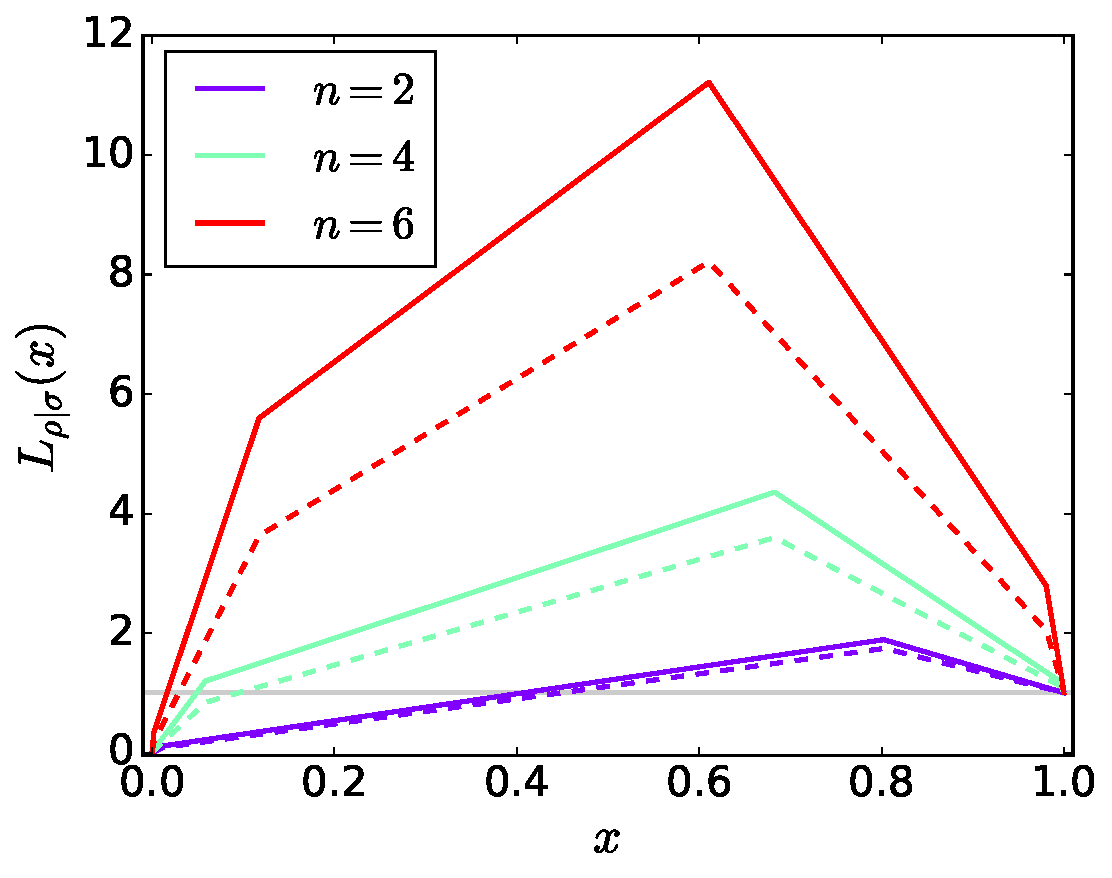
\includegraphics[scale=0.35]{figs/lc_strange.pdf}
    \caption{\textbf{A `heretical' family of Lorenz curves.} Traditionally, Lorenz curves for distributions are monotone increasing cumulant functions that reach a maximum value of $1$. In contrast, Lorenz curves for magic states break through the value of $L(x)=1$ due to the presence of negativity in the associated quasi-probability distributions. The above family of curves correspond to multiple copies of noisy Strange states $\rho\coloneqq\rho_{\rm{S}}(\epsilon)^{\otimes n}$ (\cref{eq:noisysn}) for $n=2,4,6$ within a particular stabilizer fragment ($\sigma = \id/3$). Solid lines represent pure Strange states, while dashed lines represent $\epsilon$-noisy Strange states with depolarising error $\epsilon = 0.1$.
    }
    \label{fig:lcs}
\end{figure}

However, relative majorization is usually considered for probability distributions, so we need to verify that the same Lorenz curve conditions apply to quasi-probability distributions before proceeding with our analysis. This can be done from first principles, but a simpler way is see that this holds is to reduce to the problem of genuine distributions by first `masking' the negativity in the quasi-probability distribution $\w$ using the reference distribution $\r$ and then applying the conditions for relative majorization. This negativity masking then gives the following result.

\begin{lemma} Let $\w \in \mathbb{R}^n,\w'\in \mathbb{R}^m$ be quasi-distributions, and let $\r \in \mathbb{R}^n, \r' \in \mathbb{R}^m$ be probability distributions with non-zero components. Then $(\w, \r) \succ (\w', \r')$ if and only if $L_{\w|\r}(x) \ge L_{\w |\r}(x)$ for all $x \in [0,1]$.
\end{lemma}
 
 \begin{proof}
Since the components of $\r$ are strictly positive, there always exists an $\epsilon >0$ such that $\w_\epsilon \coloneqq \epsilon \w + (1-\epsilon) \r$ is a genuine probability distribution. A similar result holds for $\w'$ and $\r'$ and we choose $\epsilon$ sufficiently small so that both $\w_\epsilon$ and $\w_\epsilon'$ are probability distributions. We now have that $(\w , \r) \succ (\w', \r')$ if and only if $(\w_\epsilon , \r) \succ (\w_\epsilon', \r')$. This equivalence holds because there exists a stochastic map $A$ such that $A \w = \w'$ and $A \r = \r'$ if and only if 
\begin{equation}
A[\epsilon \w + (1-\epsilon) \r] = \epsilon \w' + (1-\epsilon) \r'\mbox{ and } A\r = \r'.
\end{equation}
In terms of a Lorenz curve condition we have that $(\w_\epsilon , \r) \succ (\w_\epsilon', \r')$ if and only if $L_{\w_\epsilon |\r} (x) \ge L_{\w'_\epsilon |\r'} (x)$ for all $x \in [0,1]$. 
However, as we show in the Appendices (\cref{lemma:Lorenz_linearity}), the Lorenz curve for any quasi-probability distribution obeys the relation
\begin{equation}
L_{a \w + b \r | \r} (x) = a L_{\w|\r} (x) + bx,
\end{equation}
for any $a >0$ and $b \in \mathbb{R}$. This relation implies that
\begin{align}
L_{\w_\epsilon |\r} (x) &\ge L_{\w'_\epsilon |\r'} (x) \nonumber \\ 
&\mbox{ if and only if }& \nonumber \\
\epsilon L_{\w |\r} (x) + (1-\epsilon) x &\ge \epsilon L_{\w' |\r'} (x) + (1-\epsilon) x.
\end{align}
Finally, the $(1-\epsilon)x$ terms cancel on both sides and we get the required relative majorization conditions that $(\w, \r) \succ (\w', \r')$ if and only if $L_{\w | \r} (x) \ge L_{\w' | \r'}(x)$ for all $x \in [0,1]$, as required.
\end{proof}

With all the necessary theory in place, we now turn to magic distillation protocols.

\newpage
\section{Magic distillation bounds from majorization}
\label{sec:frag}

We can now consider how physical constraints that may be hardware specific, affect magic distillation rates. These are not a priori encoded in the formulation of the magic theory, and constitute additional physical conditions on top of the underlying resource-theoretic accounting. For example, there may be non-trivial thermal noise in the physical set-up or the accessible operations, there might be strong bias in the noise present, or we might be limited in how easily certain gates can be realised.~\cite{Aliferis_2008, Stephens_2013, Li_2015, Babbush_2018, Tuckett_2019, Guillaud_2019, Fowler_2019}.

In~\cref{sec:stab} we shall focus on the energetic costs of a protocol, that are defined due to the specific Hamiltonian that the system possesses. However, before that, in this section we encode physical constraints at a more abstract level in terms of the fixed-point structure of  the actual operations that are accessible to us. We show that any magic theory can always be decomposed in terms of `sub-theories' with a particular fixed-point structure. This section therefore exploits $\mathbf{d}$--majorization, while in~\cref{sec:stab} we drop the requirement of fixed-points and instead use the full relative majorization relation.
 
 We begin by defining the following kind of sub-theory of any magic theory $\R$.
\begin{definition}\label{def:sigmafrag}
   Given a theory of magic $\R = (\F, \O)$, the \emph{$\sigma$--fragment of $\R$} is the sub-theory $\R_\sigma = (\F, \O_\sigma)$, in which the free operations are 
   \begin{equation}
        \O_\sigma \coloneqq \{ \E \in \O: \E(\sigma) = \sigma \},
    \end{equation}
namely those free operations that leave the distinguished state $\sigma \in \F$ invariant.
\end{definition}
This notion provides a simple way to break up any theory into smaller, more manageable parts. Moreover, the union over all fragments returns the parent theory, so we are not discarding any information by breaking up the theory in this way. We make this statement precise as follows.
\begin{theorem}\label{thm:frag}
    Let $\R = (\F, \O)$ be a theory of magic.
Then a transformation $\rho \rightarrow \tau$ is possible in $\R$ if and only if the transformation $\rho \rightarrow \tau$ is possible in at least one $\sigma$--fragment of $\R$.
\end{theorem}
The proof of this is straightforward.
\begin{proof}
   Suppose the interconversion is possible in a $\sigma$--fragment via some $\E \in \O_\sigma$. But since $\O_\sigma \subseteq \O$ it is also possible in $\R$. Conversely, suppose the transformation is possible in $\R$ via some $\E$ in $\O$. The free states $\F$ are a closed, bounded set and moreover the image of $\F$ under the map $\E$ is in $\F$. By the Brouwer Fixed-Point theorem~\cite{cit:brouwer} this mapping must therefore have a fixed point $\sigma \in \F$. Therefore, $\E \in \O_\sigma$ and the interconversion is possible in this fragment.
\end{proof}
One can compare with resource monotones, which are also called resource measures. A complete set of measures $\{\M_i\}_i$ is such that $\rho \rightarrow \sigma$ if and only if $\M_i(\rho) \ge \M_i(\sigma)$ for all $i$. The above set of sub-theories can therefore be viewed as a complete set of ``co-measures'' for the theory, where the parent resource theory's complex pre-order of states is mapped to a simpler pre-order for a particular fragment. In the next section we show that this pre-order for a given fragment can always be approximated by a majorization pre-order, and from this we can compute magic distillation bounds.


\begin{figure}[t]
    \centering
        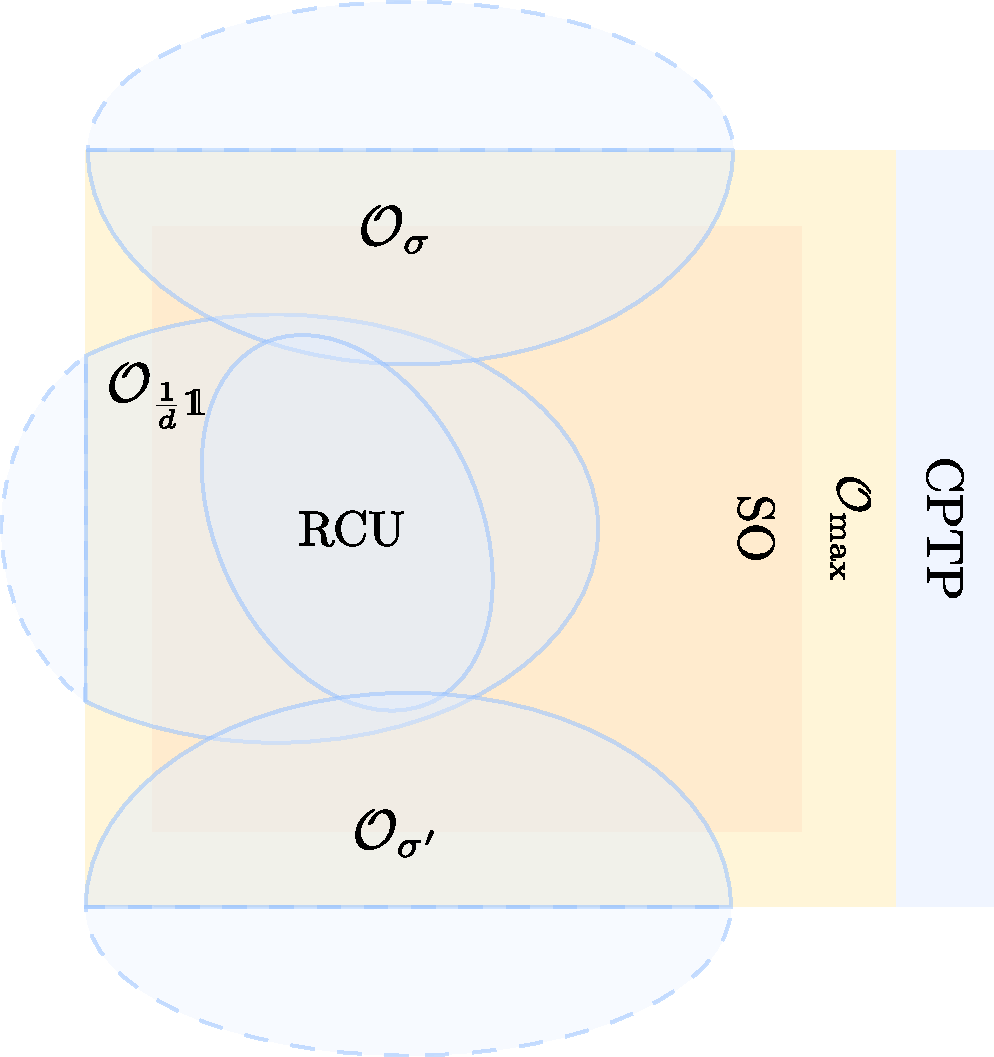
\includegraphics[scale=0.3]{figs/operations.pdf}
    \caption{\textbf{Decomposition of a magic theory $\R$ into $\sigma$--fragments.} 
	Examples of magic theories ($\so$: Stabilizer operations, $\Omax$: Completely positive-Wigner-preserving operations, $\rcu$: Random Clifford Unitaries -- subclass of $\so$) are labelled, with other established magic theories also contained within the yellow regions.
    We introduce $\sigma$--fragments $\O_\sigma$ defined for all free states $\sigma$ that cover $\Omax$. 
    Each $\O_\sigma$ is extensible to a set of stochastic maps outside the $\cptp$ operations.
    Within each $\sigma$--fragment, relative majorisation can be used allowing for a tractable approach towards the study of magic state interconversions.
    }
    \label{fig:zoo}
\end{figure}

\subsection{Majorisation of negative Wigner distributions within $\sigma$--fragments}
\label{sec:major_frag}

We consider some $\sigma \in \F$, and its corresponding fragment $\R_\sigma$. We are interested in the ability to transform many copies of some noisy magic state $\rho$ towards a more pure form of magic. The state $\rho$ is assumed to have negativity in the Wigner representation, so $W_\rho(\x) < 0$ for some regions of $\x \in \P_d$. The state $\sigma$ is assumed to have a Wigner distribution with $W_\sigma(\x) > 0$ for all $\x$ in the phase space\footnote{Any non-full rank state $\sigma$ can be handled as a limiting case in which we first add an infinitesimal fraction of depolarising noise $\epsilon (\id/d)$ and then take $\epsilon \rightarrow 0$ in the end.}.

The free operations within the magic theory $\R$ are represented by stochastic maps, and within $\R_\sigma$ by stochastic maps that leave $W_\sigma(\x)$ invariant. Therefore, a necessary condition for magic state transformations $\rho_1 \rightarrow \rho_2$ within $\R_\sigma$ will be that 
\begin{equation}
	W_{\rho_1} \succ_{W_{\sigma}} W_{\rho_2},
\end{equation}
or put another way, that the quasi-distribution $W_{\rho_1}$ is more ordered than the quasi-distribution $W_{\rho_2}$ relative to $W_\sigma$. To simplify notation, we denote by $L_{\rho | \sigma}(x)$ the Lorenz curve $L_{W_{\rho} | W_{\sigma}} (x)$, and therefore have that
\begin{equation}
\rho_1 \rightarrow \rho_2 \mbox{ within }\R_\sigma \mbox{ implies } L_{\rho_1 |\sigma} (x) \ge L_{\rho_2 |\sigma} (x),
\end{equation}
for all $x \in [0,1]$, which restricts the transformations that are possible.

  Note, however, that this is not a single numerical constraint, but a family of constraints. For $n$ copies of a qudit system of dimension $d$ the number of terms in $W_{\rho}$ is $d^{2n}$, so imposing the Lorenz curve condition corresponds to \emph{exponentially} many constraints. However,  before computing explicit examples, in the next section we highlight how these majorization constraints relate to other known monotones.

\subsection{Basic monotones for magic states in a particular fragment}
\label{sec:monotones_frag}

In this section, we state some generic aspects of Lorenz curves for magic states. These allow us to interpret previous magic monotones in a new light. The first result gives an extremely simple way to see that the sum-negativity of a magic state is a monotone.

\begin{lemma} Relative majorization in any fragment implies the monotonicity of sum-negativity. 
\end{lemma}
\begin{proof}
	The sum-negativity of a magic state $\rho$ can be written as $sn(\rho) =\frac{1}{2} (\sum_{\x} |W_\rho(\x) | - 1)$.
We make use of the $L_1$-norm form of relative majorization, (see~\cref{app:major}), which states that $\p \succ_{\r} \q$ if and only if
	\begin{equation}
\sum_k | p_k - r_k t | \geq \sum_k | q_k - r_k t |,
\end{equation}
for all $t\in \mathbb{R}$. Choosing $t=0$ we get the single condition that $\sum_k |p_k| \ge |\sum_k |q_k|$, independent of the choice of $\r$. Applying this to the Wigner quasi-distributions of two quantum states immediately gives the result.
\end{proof}

If we have a magic state $\rho$ that has negativity in its Wigner representation, then, as discussed, its Lorenz curve over-shoots $1$ and reaches a non-trivial maximum $L_\star$ that depends on the particular state. There is an simple relation between $L_\star$ and sum-negativity or mana, which is provided by the following result. 
\begin{theorem}\label{lem:lcmax}
	Given a magic state $\rho$, the maximum $L_\star$ of its Lorenz curve $\lc{\rho}{\sigma}(x)$ is independent of the $\sigma$--fragment and equal to $1+\sn{\rho}$. Moreover, the majorization constraint is stronger than mana in every fragment.
\end{theorem}
The proof of this is given in~\cref{app:major}. Using the Lorenz curve perspective, it is also simple to construct new monotones. For example, within a given fragment, the area above the horizontal line $y = 1$ is another magic monotone.
\begin{lemma}
Given a magic state $\rho$ and a free state $\sigma$, let $\A_\sigma(\rho)$ be the area of the region $\{(x, y): 1 \leq y \leq L_{\rho | \sigma}(x)\}$. Then $\A_\sigma(\rho)$ is a magic monotone for $\R_\sigma$.
\end{lemma}
\begin{proof}
Consider the transformation $\rho_1 \rightarrow \rho_2$ within $\R_\sigma$. We have that $L_{\rho_1|\sigma}(x)$ is never below the curve $L_{\rho_2|\sigma}(x)$, and therefore the region above $L=1$ for $\rho_2$ is a subset of the corresponding region for $\rho_1$. Thus, $\A_\sigma(\rho_1) \geq \A_\sigma(\rho_2)$, so $\A_\sigma$ is a magic monotone in $\R_\sigma$.
\end{proof}
Note though, in contrast to mana, the area monotone is \emph{specific to the fragment}, and its value will vary as we change $\sigma$. Therefore its monotonicity is conditioned on the physics of the fragment and so provides a means to analyse magic distillation only under free operations that leave $\sigma$ invariant. One can also define an area monotone in the more general setting of relative majorization, where one drops the fixed point emphasis as in Section \ref{sec:stab}, but we do not explore this here.

\subsection{Magic distillation bounds for unital protocols}
\label{sec:unital}



We now construct magic state distillation bounds within the unital fragment ($\sigma = \I/d$). This describes distillation protocols that generate \emph{unital operations}, meaning that $\E(\I/d) = \I/d$, and includes for example all protocols built from Weyl-covariant channels~\cite{cit:gross3}. 

Our approach applies to any dimension, but for simplicity we consider qutrit magic states ($d=3$), for which a canonical magic state exists with a particularly simple Wigner distribution. This is the Strange state $|S\>$, which is given by
\begin{equation}
|S\> \coloneqq \frac{1}{\sqrt{2}} (|1\> + |2\>),
\end{equation}
in the computational basis. Its distribution $W_S(\x)$ has a single negative value of $-1/3$ at $\x =(0,0)$ and the positive value $1/6$ at all other points. We define the $\epsilon$--noisy Strange state as
\begin{equation}\label{eq:noisysn}
    \rho_{\rm{S}}(\epsilon)\coloneqq (1 - \epsilon) \ket{\rm{S}}\bra{\rm{S}} + \epsilon \frac{1}{3}\id,
\end{equation}
where $\epsilon$ is the depolarizing error parameter. One nice feature of this is that any magic state $\rho$ can be processed via Clifford operations~\cite{cit:prakash,cit:prakash2} and put into this canonical form for some $\epsilon \ge 0$.

The Wigner distribution of the single-copy, $\epsilon$--noisy Strange state  is given by
\begin{equation}
	\W[\bmx]{\rho_{\rm{S}}(\epsilon)} = (1-\epsilon)\W[\bmx]{\rm{S}\>\<\rm{S}|} + \epsilon\W[\bmx]{\frac{1}{3}\id}.
\end{equation}
with a single negative component
\begin{equation}
	- v(\epsilon) \coloneqq - \left( \frac{1}{3} -\frac{4}{9}\epsilon \right)
\end{equation} 
located at the origin $\bmx = \bmo$ and positive components
\begin{equation}
	u(\epsilon) \coloneqq \frac{1}{6} -\frac{1}{18}\epsilon
\end{equation}
at the 8 phase space points $\x \ne \mathbf{0}$. We assume that $\epsilon < 3/4$ to ensure the presence of negativity in the Wigner distribution. 

We now consider purifying $n$ copies of a noisy Strange state $\rho_{\rm{S}}(\epsilon)^{\otimes n}$ into a smaller number of copies $n'$ of a less noisy Strange state $\rho_{\rm{S}}(\epsilon')^{\otimes n'}$, with $\epsilon' < \epsilon$ and $n' \leq n$. Since we work in the unital fragment, the maximally mixed state is free and we choose to tensor in $n'-n$ auxiliary copies of it to the output. This simplifies analysis, and does not affect distillation rates as it is easy to see that
\begin{equation}
	L_{\rho |\sigma} (x) = L_{\rho \otimes \sigma |\sigma \otimes \sigma}(x),
\end{equation}
for any full-rank $\sigma \in \F$. Therefore, we compute the Lorenz curves for the transformation
\begin{equation}\label{eq:sudist}
	\rho_{\rm{S}}(\epsilon)^{\otimes n} \longrightarrow \rho_{\rm{S}}(\epsilon')^{\otimes n'} \otimes \left( \frac{1}{3}\id \right)^{\otimes (n-n')},
\end{equation}
and use them to bound the distillation rate $R(\epsilon, \epsilon') \coloneqq n'/n$.

Due to negativity, the ordering of the components of rescaled Wigner distribution $W_{\rho_n |\sigma_n}(\bmx) \coloneqq W_{\rho_n}(\bmx)/W_{\sigma_n}(\bmx)$, for $\rho_n = \rho_S(\epsilon)^{\otimes n}, \sigma_n = \sigma^{\otimes n}$, depends on whether $-v(\epsilon)$ appears to an even or odd power in the expression of~\cref{eq:wigu}. Treating the Wigner distributions as vectors, the component values $w_i$ and associated multiplicities ($m_i$) in the $n$--copy case are found to be 
\begin{align}
	m_i &= 8^{i}\binom{n}{i}, \\
	w_i &= u^{i}(-v)^{n-i}, \label{eq:wigu}
\end{align}
where index $i$ runs through $0, \dots, n$, and we assume for simplicity that $n$ is even and $\epsilon \leq 3/7$, which implies that $v \geq u$.
The details of this are provided in~\cref{app:lcsu_technical}.

The Lorenz curve $L_{\rho_n|\sigma_n}(x)$ reaches a maximum value of
\begin{align}\label{eq:lcsu_max}
	L_\star &\coloneqq L_{\rho |\sigma} (x_\star) = \sum_{i = 0}^{n/2} m_{2i} w_{2i} \nonumber\\
	&= \frac{1}{2} + \frac{1}{2}\left(\frac{15 - 8\epsilon}{9}\right)^n > 1,
\end{align}
which occurs at $x=x_\star$ given by
\begin{equation}
	x_\star = \frac{1}{2} + \frac{1}{2}\left(\frac{7}{9}\right)^n.
\end{equation}

Distillation bounds can be obained from any location of the Lorenz curve, including the region around the peak, by imposing the constraint that the Lorenz curve of the input state never dips below the curve of the output. In particular a compact constraint can be obtained by considering the initial slopes of the two Lorenz curves. 

The first elbow coordinates for $\rho_S(\epsilon)^{\otimes n}$ are given by $(1/9^n, v(\epsilon)^n)$, while for $\rho_S(\epsilon')^{\otimes n'}$ by $(1/9^{n'}, v(\epsilon')^{n'})$, and by considering the slope of the line segment joining this first elbow to the origin we can use~\cref{prop:first_elb} in the Appendices, to bound $R(\epsilon, \epsilon')$. We find that
\begin{equation}
	R(\epsilon, \epsilon') \leq \frac{\ln (3-4\epsilon)}{\ln (3-4\epsilon')}.
\end{equation}
For the limiting case of pure magic states on the output ($\epsilon'=0$), this simplifies to
\begin{equation}
	R \leq 1 + \frac{\ln (1 - \frac{4}{3} \epsilon)}{\ln 3}.
\end{equation}
This can be compared to other known distillation bounds coming from mana and thauma~\cite{Wang_2020}. The mana bound can be directly calculated as
\begin{equation}
	R \leq \frac{\mana{\rho_{\rm{S}}(\epsilon)}}{\mana{\rho_{\rm{S}}(0)}} = 1 + \frac{\ln \left(1 - \frac{8}{15}\epsilon \right)}{\ln \frac{5}{3}}.
\end{equation}
The recently introduced max--thauma~\cite{Wang_2020} is defined as
\begin{equation}
	\theta_{\rm{max}}(\rho) \coloneqq \log_2{\min{\{2\hspace{1pt}\sn{V}+1 : V \geq \rho\}}}
\end{equation}
and can be calculated numerically via a semi-definite program. For the noisy Strange state, the max--thauma bound coincides with the mana bound, and we find that they are both looser than the majorization bound we derived via the first elbow constraint as shown in~\cref{fig:distill_bounds}. 

This figure includes numerical estimates of the optimal majorization bounds $R_{\rm{opt}}$ obtained by considering the full Lorenz curve, which show that the first elbow constraint can be further improved.
\begin{figure}[t]
    \centering
    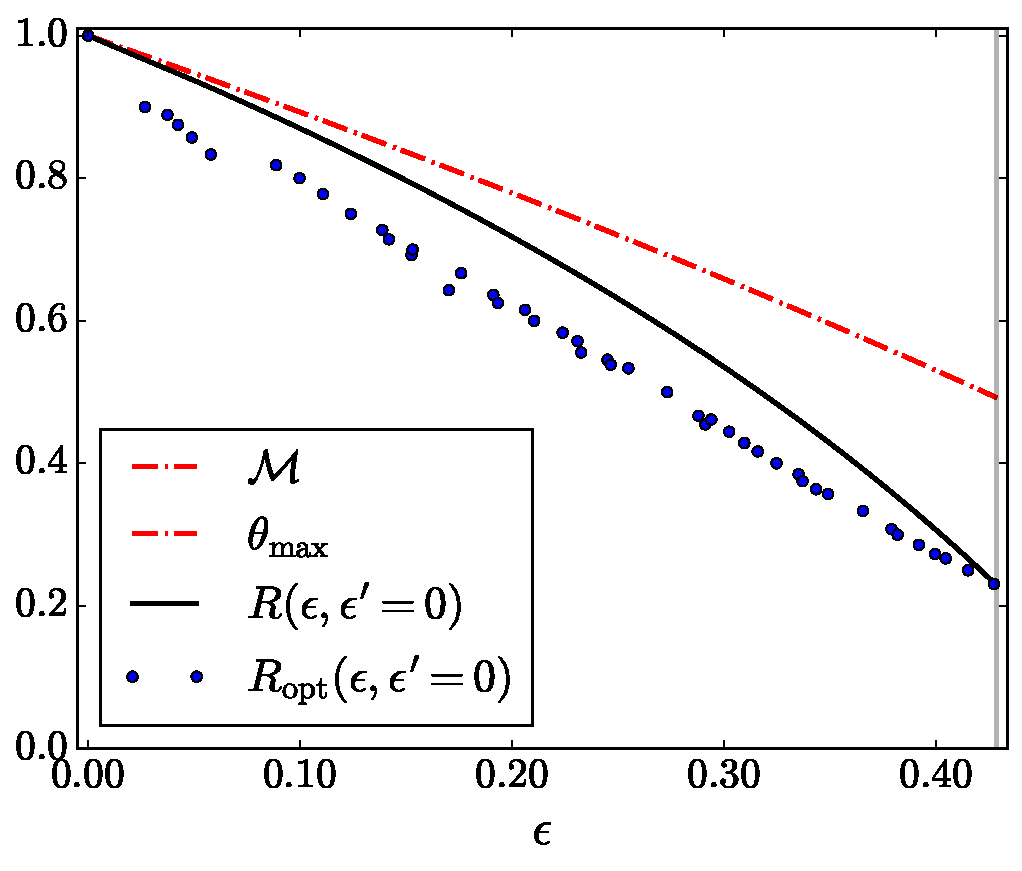
\includegraphics[scale=0.35]{figs/distill_bounds.pdf}
    \caption{\textbf{Distillation bounds in the unital fragment.} Distillation bounds obtained by the first elbow majorisation constraint $R$, mana $\M$ and max--thauma $\theta_{\rm{max}}$ are plotted for $\epsilon' = 0$, up to error $\epsilon = 3/7$.
    Majorisation provides stricter rates than the global mana and max--thauma bounds.
    Numerical bounds $R_{\rm{opt}}$ obtained by full Lorenz curve comparison for some Strange state purification processes with even number of copies $m,n \leq 30$ highlight that the first elbow constraint can be improved.
    }
    \label{fig:distill_bounds}
\end{figure}

In the next section, we loosen the restriction of working in a fixed fragment, and instead use the full structure of relative majorization to obtain bounds that incorporate energetic aspects of a magic state protocol.

\newpage
\section{Temperature-dependent bounds for magic state distillation protocols}
\label{sec:stab}

We now consider a magic distillation protocol on multiple identical qudits in a noisy magic state $\rho(\epsilon)$, with noise parameter $\epsilon$, sending 
\begin{equation}
\rho(\epsilon)^{\otimes n} \longrightarrow \E(\rho(\epsilon)^{\otimes n}) =\rho(\epsilon')^{\otimes m}
\end{equation}
with $n \gg 1$, $\epsilon' <\epsilon$ and $\E$ denoting the quantum channel induced by the protocol. We can now provide distillation bounds that depend on energetic and entropic aspects of the protocol. We do this relative to a reference temperature that can be chosen freely. The key idea is that the physical measures associated with this protocol are determined by how $\E$ would disturb a reference equilibrium state $\tau$ to some different state $\tau'$, if the protocol had been applied to this reference state instead of the $n$-copy magic state. 

More precisely, we assume each qudit has Hamiltonian $H$ and we choose some temperature $T = (k\beta)^{-1}$ where $k$ is Boltzmann's constant and $\beta$ the inverse temperature. The reference equilibrium state of the $n$ qudits is given by
\begin{equation}
\tau^{\otimes n} = \left ( \frac{e^{-\beta H}}{\Z} \right )  ^{\otimes n}.
\end{equation}
Since we are concerned with magic distillation we may assume that the reference state $\tau$ is not a magic state, so it has a non-negative Wigner distribution, and we shall further assume that it is a full-rank stabilizer state for the qudit. 

A given magic protocol on the $n$ qudits will correspond to a quantum channel $\E$. Our analysis associates to this protocol energy/entropy measures by considering how $\E$ transforms this reference equilibrium state. We first note that we can assume without loss of generality that $U_\pi\E(X) U_\pi^\dagger = \E(X)$ for all $X$ and any permutation $U_\pi$ of the $m$ output subsystems. This is justified because the protocol on the input magic state results in state $\rho(\epsilon')^{\otimes m}$, which is invariant under permutations. Therefore, we are always allowed to symmetrise the output $\E(X)$ by performing a group average over the permutation group for the output systems without changing the performance of the distillation protocol on $\rho(\epsilon)^{\otimes n}$. Thus, we can assume that $\E$ always outputs a symmetric state in general.

This means in particular that $\E(\tau^{\otimes n})$ is a symmetric state on $m$ subsystems, so by the quantum de Finetti theorem~\cite{christandl_2007} we have that for $m \gg 1$
\begin{equation}
\E(\tau) \approx \int d\mu(x) \tau_x^{\prime \otimes m},
\end{equation}
where $d\mu(x)$ is a probability measure over a set $\{\tau'_x\}$ of single qudit states. This makes the setting easier to handle, although we make one more simplifying assumption as explained in the next section.

\subsection{Free energy and sub-linear correlations in the thermodynamic limit}
To simplify our analysis we will make the following physical assumption. We assume that in the asymptotic/thermodynamic limit $n,m \rightarrow \infty$ that correlations generated on the reference equilibrium state are negligible. This implies that $d\mu(x)$ is peaked on a particular state $\tau'$, and $\E(\tau) = \tau'^{\otimes m}$. Physically, this is a natural scenario -- for example, in the context of traditional thermodynamics, it states that the output system is well-described by intrinsic variables that do not scale in $m$, and correlations are sub-linear in $m$. This allows us to compute a free energy per qudit of the output state.

The case of non-trivial correlations in the thermodynamic limit can also be considered, but leads to a more complex analysis within our majorization framework of Wigner distributions. In this direction, we highlight recent work in majorization in which stochastic independence and correlations are analysed. In particular, it has been shown that stochastic independence (no correlations) of independent distributions can be viewed as a resource in an extension of catalytic majorization, and leads to a single-shot operational interpretation of the Shannon entropy~\cite{muller_2015, muller_2016, muller_2019}.

Our analysis will depend on the energetic properties of the probe state $\tau$ and the output state $\tau'$.
For the state $\tau = e^{-\beta H}/\Z$, the Helmholtz free energy $F$ is given by
\begin{equation}
	F \coloneqq \tr[H \tau] - \beta^{-1}S(\tau) = -\beta^{-1}\log{\Z},
\end{equation}
which can be obtained from the internal energy via a Legendre transform~\cite{Pathria_1997}.

The protocol transforms the equilibrium as $\tau^{\otimes n} \rightarrow \E(\tau^{\otimes n}) = \tau^{\prime \otimes m}$.  The protocol does not, on its own, generate magic and so we assume the output state $\tau'$ is also a Wigner-positive state. However, this is generally a \emph{non-equilibrium} state for the system. Despite this, the distillation bounds that we derive take a particularly simple form if we associate an effective Hamiltonian $H'$ to the output state by considering the change $H \rightarrow H'$ such that equilibrium is restored at the reference temperature $T$. This Hamiltonian is defined by the expression $\tau' = e^{-\beta H'}/\Z'$, and has free energy $F' = -\beta^{-1} \log \Z'$.

\subsection{Temperature-dependent distillation bounds}

W \nick{what is W?} can specify energetic details of a protocol through how much it would disturb some reference equilibrium state. The magic state transformation is then considered relative to the equilibrium transformation, and can be recast via the Wigner representation into a relative majorization statement $(\w, \r) \succ (\w', \r')$ where $\w, \w'$ are quasi-distributions corresponding to the magic transformation, while $\r, \r'$ correspond to the transformation of the reference equilibrium state. 

This leads to the following magic distillation bound that combines computational measures $\epsilon,\epsilon'$, with terms that depend on the Hamiltonian and reference temperature $T$ of the physical system. We state the result for the case of qutrits, but a similar analysis is possible for general qudits.

\begin{theorem}\label{thm:free-energy}
	Consider a magic distillation protocol on qutrits that transforms $n$ copies of an $\epsilon$--noisy Strange state into $m$ copies of an $\epsilon'$--noisy Strange state, with depolarising errors $\epsilon' \leq \epsilon \leq 3/7$. We also allow pre/post-processing by local Clifford unitaries.
	
	Let $T =(k\beta)^{-1}$ be any finite temperature for the physical system and let $H= \sum_{k \in \mathbb{Z}_3} E_k |E_k\>\<E_k|$ be the Hamiltonian of each qutrit subsystem in its eigen-decomposition.
Assume that in the thermodynamic limit ($n,m \gg 1$), the protocol applied to the equilibrium state $\tau^{\otimes n} = (e^{-\beta H}/\Z)^{\otimes n}$ maps $\tau^{\otimes n} \longrightarrow \tau^{\prime \otimes m}$, where we write $\tau' = e^{-\beta H'}/\Z'$ for some Hermitian $H'$.

Then the asymptotic magic distillation rate $R = m/n$ is bounded as
\begin{equation}\label{eq:rate_bounds_proof}
	R \leq \dfrac{\ln \big( 1-\frac{4}{3}\epsilon \big) + \beta (\phi - F)}{\ln \big( 1-\frac{4}{3}\epsilon' \big) + \beta (\phi' - F')},
\end{equation}
where $F$ is the free energy of $\tau$,  and 
\begin{equation}
	\phi = -\beta^{-1} \log \zeta
\end{equation}
with $\zeta$ given by the expressions
\begin{align}
	\zeta &= \sum_{k\in \mathbb{Z}_3} \alpha_k e^{-\beta E_k}, \nonumber\\
	\alpha_k &= \<E_k| A_{\x_\star} |E_k\>,
\end{align}
and $W_\tau(\x)$ attaining a minimum at $\x=\x_\star$. The primed variables are defined similarly for the output system.
\end{theorem}
\noindent The proof of this is provided in~\cref{thm:free-energy-bound-proof}, and follows a similar line as taken for our unital protocol bound.

The above bound depends on: 
\begin{itemize}
\item Quantum computational measures $\epsilon, \epsilon'$,
\item Thermodynamic quantities $\beta, F, F',$
\item Intermediate terms $\phi, \phi'$. 
\end{itemize}
The intermediate terms specify how the energy eigenbasis of the system $\{|E_k\>\}$ relates to the computational stabilizer basis $\{|k\>\}$.  In particular, the term $\phi$ quantifies to what degree a sharp energy value can be ascribed to the negativity in the Wigner representation. Its form is similar to $F$, so $\phi$ can informally be viewed as a `magic free energy' term. 

The coefficients $\alpha_k$ may be negative for some $k$, when the Hamiltonian has non-stabilizer eigenstates, but the quantity $\phi$ is always well-defined, since the function $\zeta$ is always positive for $\tau$ in the interior of $\F$. The quantity $\phi$ can diverge if the state $\tau$ acquired zero Wigner components, which occurs for $\tau$ on the boundary of the set of Wigner-positive states, and is not defined outside of $\F$. Finally, if $H$ has a stabilizer eigenbasis then $\phi = E_i$ for some $i$, independent of the temperature $T$. Details of this are provided in Appendix \ref{app:lcst_technical}.

\subsection{Technical aspects of the bound}
Similar to the unital protocol bounds, the above result is based on only part of the Lorenz curves and so can certainly be tightened with further analysis. The primary role of the pre/post-processing by Clifford unitaries in~\cref{thm:free-energy} is to simplify the form of the bound, and allow it to be expressed in terms of the free energy per particle in a way that does not depend on the parameters $\epsilon, \epsilon', \beta$ in a complex form. In Appendix \ref{app:lcst_technical}, we give bounds in which one does not include these Clifford changes of basis (see Theorem \ref{thm:no-processing}), and which have a more non-trivial dependency on the parameters.


\iffalse
\begin{figure}[t!]
    \centering
    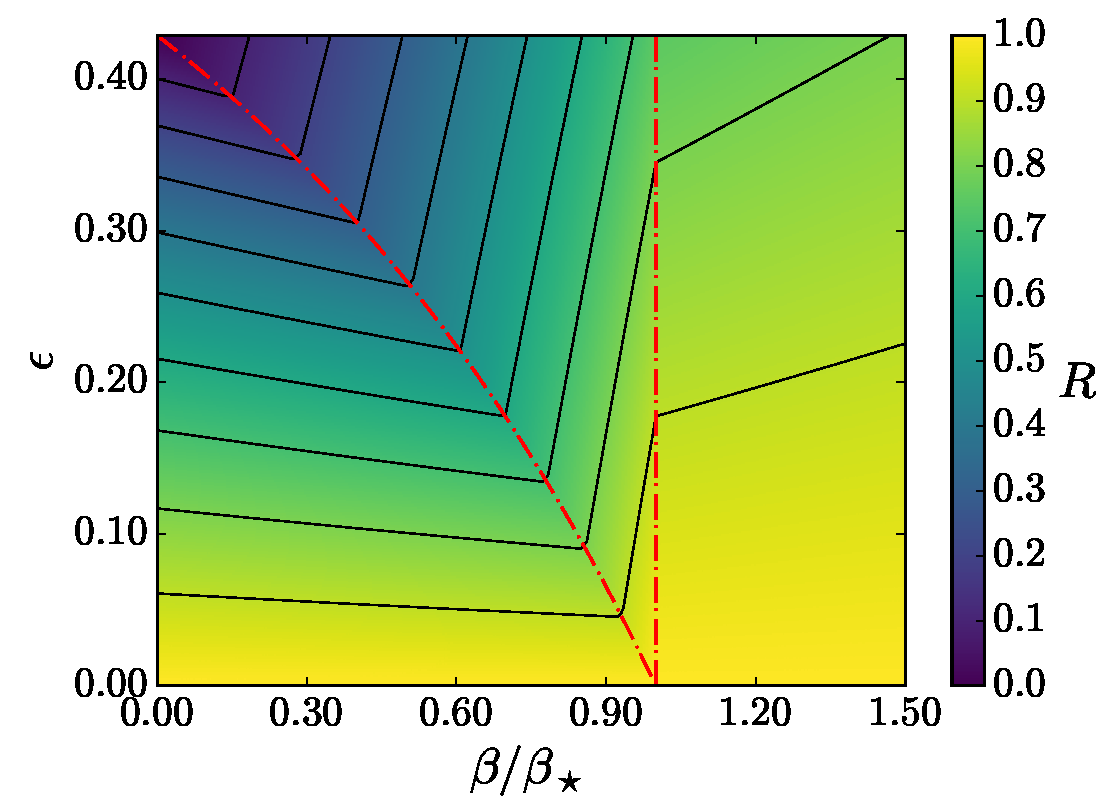
\includegraphics[scale=0.4]{figs/rate_scatter.pdf}
    \caption{\textbf{Temperature-dependent bounds for magic distillation.}
  Shown is a contour plot of the bound on $R(\epsilon, \beta)$ for $H = H' = \sum_{k \in \mathbb{Z}_3} k |k\>\<k|$ and $\epsilon' = 0$, where $\beta$ is the inverse temperature and $\epsilon$ the depolarising error of the input magic state. The relevant data from the spectrum of the qutrit operator $H$ enters in via $\epsilon_\star(\beta)$ and $\beta_\star$. The vertical dashed line is the `Landauer-like' temperature threshold $\beta_\star$ and the diagonal dashed curve corresponds to the noise threshold $\epsilon_\star(\beta)$ for $\beta \leq \beta_\star$. \nick{Refer to definitions of starred quantities} The $\beta = 0$ line corresponds to the regime in which the magic protocol corresponds to a unital channel.
    }
    \label{fig:rate_contour}
\end{figure}
\fi

\begin{figure}[t!]
    \centering
    \subfigure[][]{%
    \label{fig:noCliff}%
    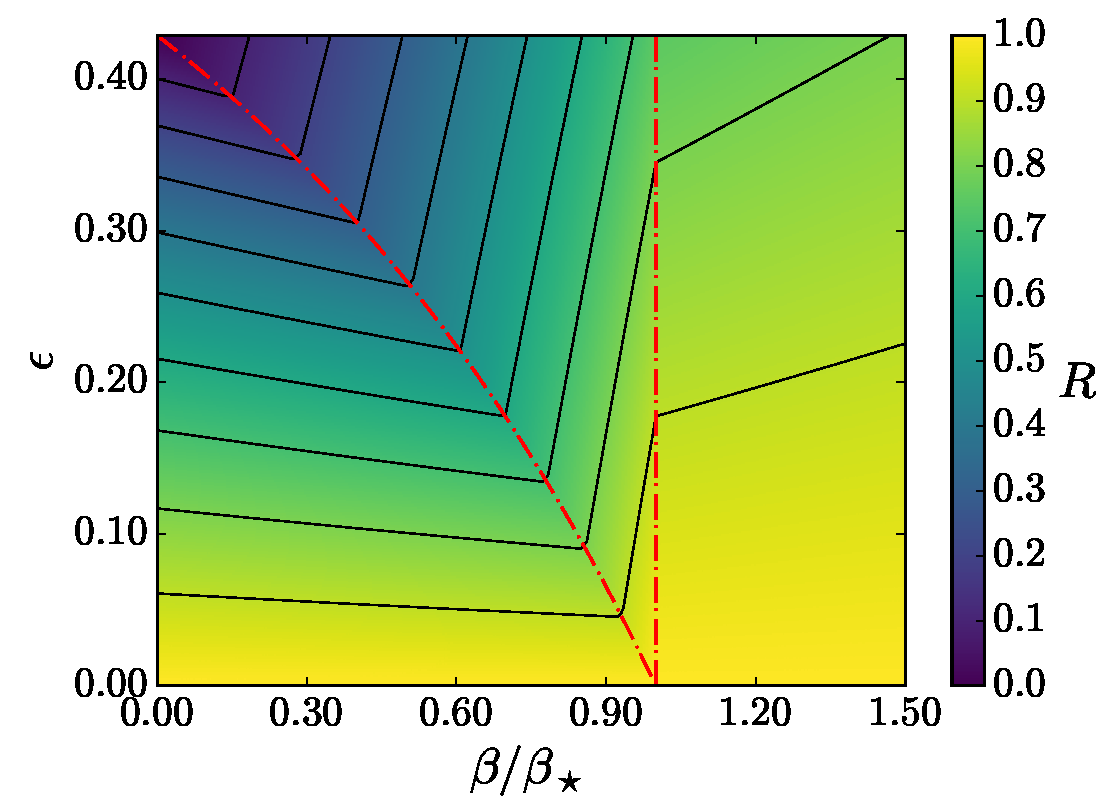
\includegraphics[scale=0.4]{figs/rate_scatter.pdf}}\\
    \subfigure[][]{%
    \label{fig:Cliff}%
    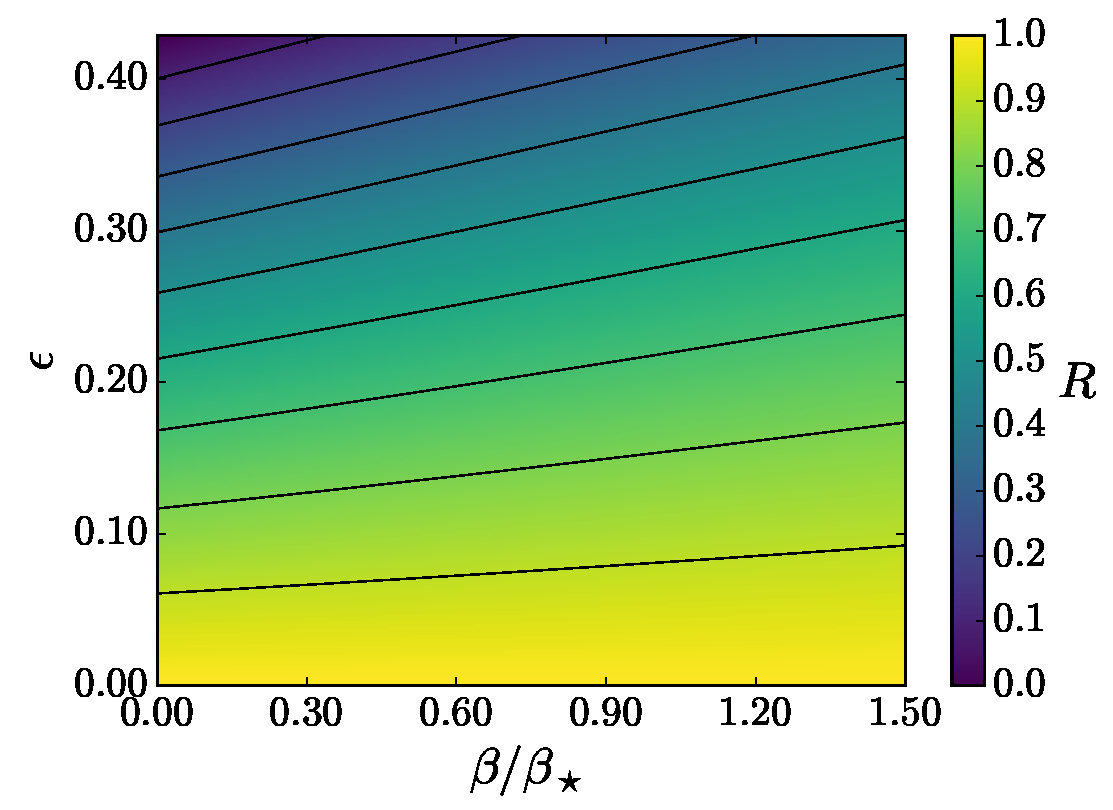
\includegraphics[scale=0.4]{figs/rate_scatter_cliff.pdf}}
    \caption{\textbf{Temperature-dependent bounds for magic distillation.} Shown are two contour plots of the bound on $R(\epsilon, \beta)$ for the case $H = H' = \sum_{k \in \mathbb{Z}_3} k \ketbra{k}$ and $\epsilon' = 0$, where $\beta$ is the inverse temperature and $\epsilon$ is the depolarising noise of the input magic state. 
The top figure \subref{fig:noCliff} does not use any changes of Clifford basis, and the form of the bound depends on both the noise parameter and temperature. The curved dashed line is $\epsilon_\star(\beta)$ is given by Equation \ref{eq:threshold} and $\beta_\star = (kT_\star)^{-1}$ is given by $E_2-\phi = kT_\star \ln 2$. 
In the bottom figure \subref{fig:Cliff} Clifford processing is used resulting in a smoother bound. In both figures the $\beta = 0$ line correspond to the unital bounds.}
    \label{fig:rate_contour}
\end{figure}


The analysis makes other simplifying assumptions that could easily be dropped, at the price of more complex expressions. We could perform similar analysis for general qudits, and different choices of magic states, for example. It might also be of interest to consider other choices of reference states $\tau$ that are more appropriate to the hardware physics, for example for photonic set-ups.

The assumption that is more non-trivial is that we neglect correlations in the reference state in the thermodynamic limit. However for more general scenarios one could make use of variational tools such as the Bogoliubov inequality~\cite{bogolyubov_1966} for approximating the free energy of a system via product states, to obtain similar bounds.





\subsection{Distillation bound for special cases}

The simplest special case to consider is where the Hamiltonian $H$ is diagonal in the computational basis, and $H=H'$, implying that the protocol leaves the reference equilibrium state unchanged, hence it corresponds to a Gibbs-preserving map~\cite{faist_2015}. For the limiting case of $\epsilon' \rightarrow 0$ we obtain~\cref{fig:rate_contour} which is a contour plot of the bound on $R$ as a function of inverse temperature $\beta$ and the depolarising error $\epsilon$ for the noisy input magic states. In this figure we show both the bounds with Clifford basis changes and without them. 


In the more general case, $\Delta F \coloneqq F' - F \ne 0$ and so the protocol, when applied to the reference state, adds/extracts free energy from the system. 



\begin{figure}
    \centering
    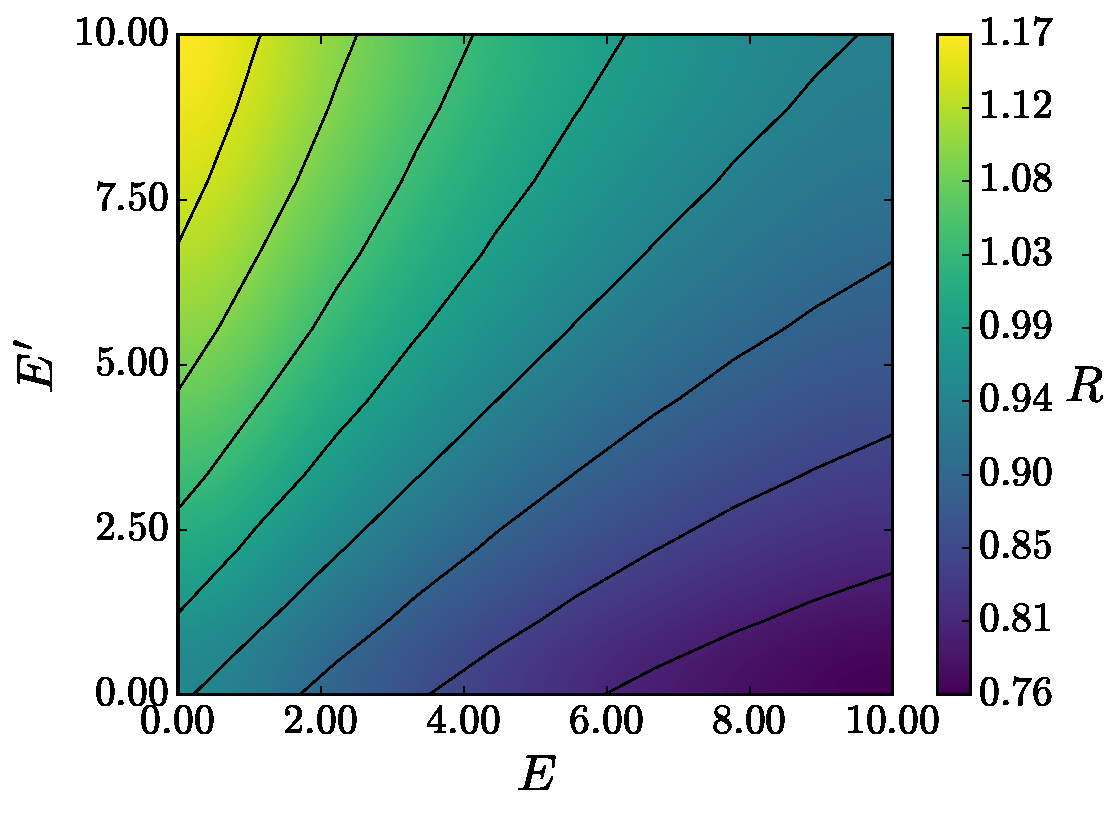
\includegraphics[scale=0.4]{figs/test/R_vs_E1.pdf}
    \caption{Here, $(\epsilon, \epsilon', \beta) = (0.1, 0.0, 0.2)$, $H = \rm{diag}(0,E,10)$ and $H' = \rm{diag}(0,E',10)$.
    }
    \label{fig:rvse1}
\end{figure}

\begin{figure}
    \centering
    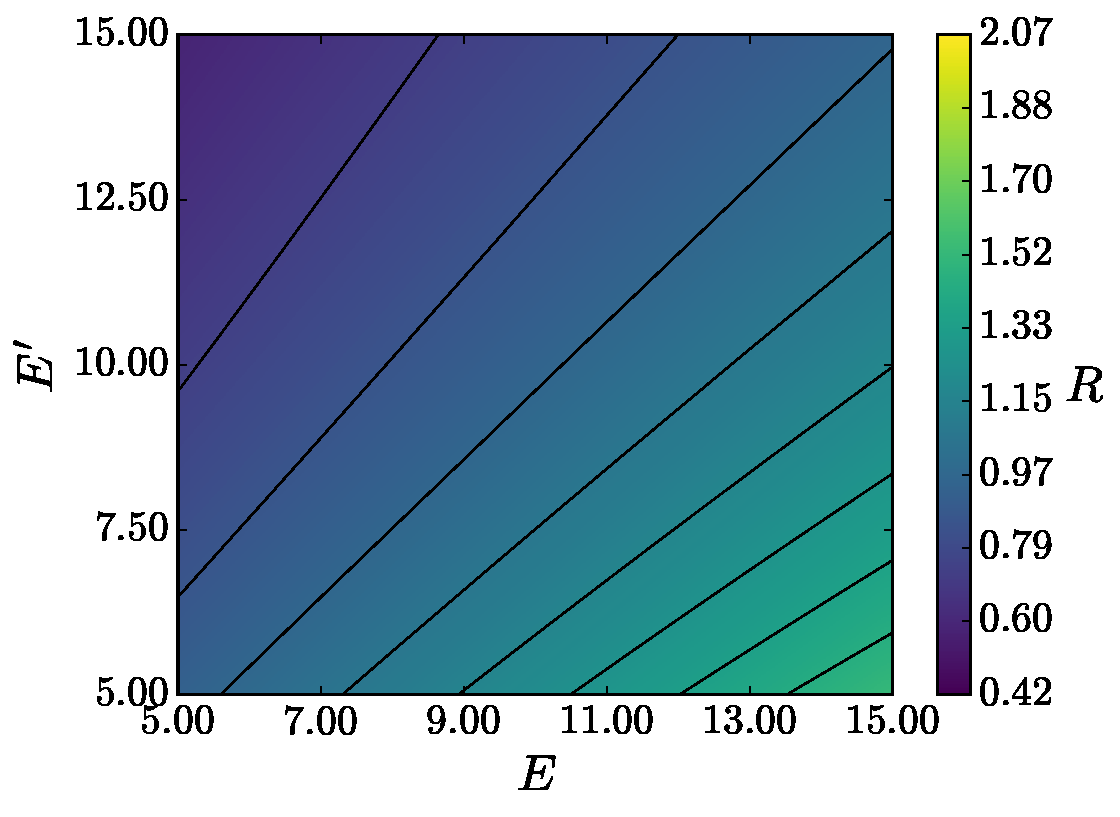
\includegraphics[scale=0.4]{figs/test/R_vs_E2.pdf}
    \caption{Here, $(\epsilon, \epsilon', \beta) = (0.1, 0.0, 0.2)$, $H = \rm{diag}(0,5,E)$ and $H' = \rm{diag}(0,5,E')$.
    }
    \label{fig:rvse2}
\end{figure}

\begin{figure}
    \centering
    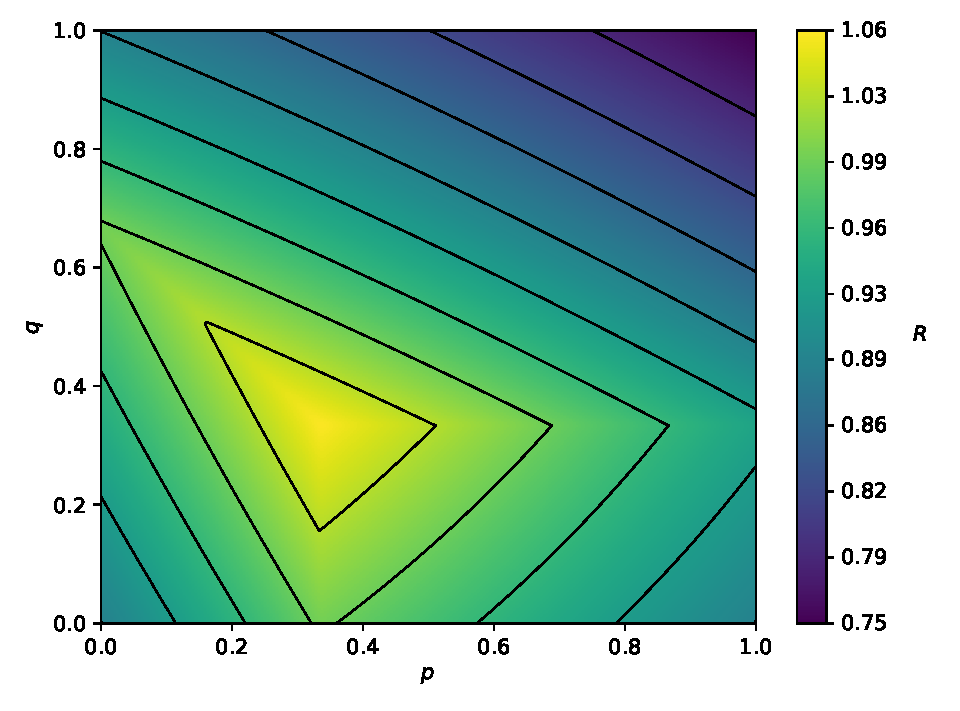
\includegraphics[scale=0.4]{figs/test/R_vs_H.pdf}
    \caption{Here, $(\epsilon, \epsilon', \beta) = (0.1, 0.0, 0.2)$, $H = {\rm{diag}}(0,1,2)$ and $H' = (1-p-q){\rm{diag}}(0,1,2)+p{\rm{diag}}(1,2,0)+q{\rm{diag}}(2,0,1)$.
    }
    \label{fig:rvsh}
\end{figure}

\begin{figure}
    \centering
    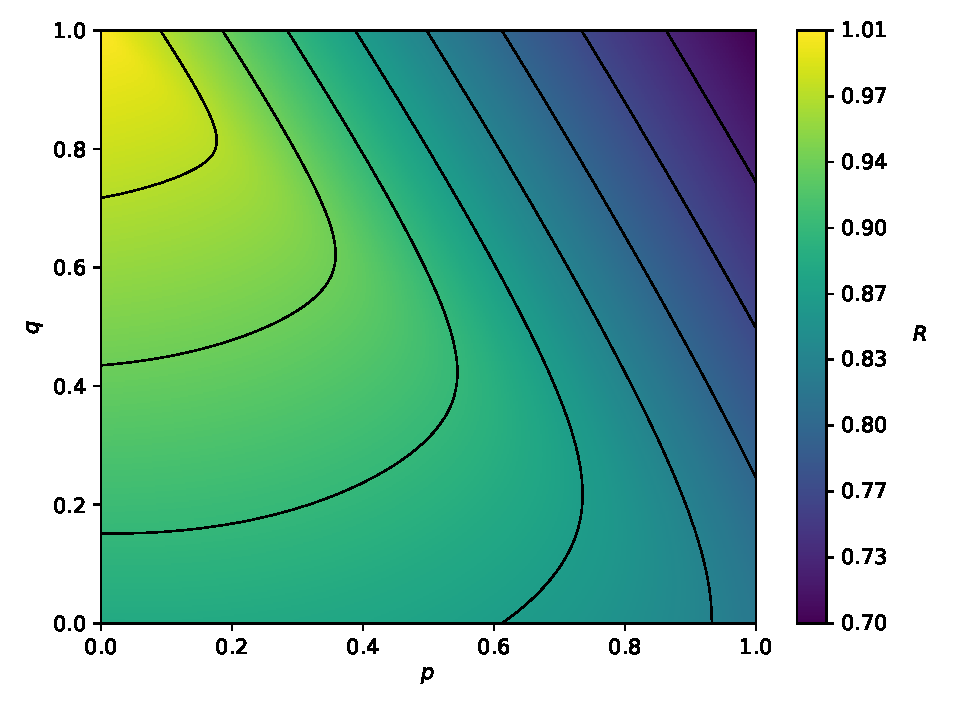
\includegraphics[scale=0.4]{figs/test/R_vs_A.pdf}
    \caption{Here, $(\epsilon, \epsilon', \beta) = (0.1, 0.0, 0.2)$, $H = A_{\bmo}$ and $H' = (1-p-q)A_{\bmo}+pA_{(1,2)}+q{\rm{diag}}(0,1,2)$.
    }
    \label{fig:rvsa}
\end{figure}

\newpage
\subsection{Single-shot divergences for quasi-distributions}
As already mentioned, the Wigner distribution is generally a quasi-distribution and so taking the Shannon entropy $H(\p) = -\sum_i p_i \log p_i$ of the Wigner distribution is not possible off of the set $\F$. However, does the same obstacle apply to Renyi entropies? The $\alpha$--Renyi entropy $H_\alpha(\p)$ is defined as
\begin{equation}
	H_\alpha(\p) := \frac{1}{1-\alpha} \log \sum_i p_i^\alpha,
\end{equation}
where $\alpha \ge 0$ and $\lim_{\alpha \rightarrow 1} H_\alpha(\p) = H(\p)$. It is clear that if we take $\alpha = 2m$ to be an even integer then $H_{2m}(\rho) := H_{2m}(W_\rho(\x))$ is always a well-defined function on Wigner quasi-distributions. However, it still remains to link such expressions to majorization of quasi-distributions.
 
In this direction, we first note that the analysis for the temperature-dependent bound given by Equation (\ref{eq:rate_bounds_proof}) implicitly makes use of the single-shot Renyi divergence $D_\infty (\p ||\r)$, which is given by
\begin{equation}
D_\infty (\p ||\r) = \log \max_i \frac{p_i}{r_i}.
\end{equation}
This motivates defining the following \emph{Wigner divergence} $D_\infty(\rho, \tau) := D_\infty (W_\rho(\x) || W_\tau (\x))$ on all quantum states. In Appendix~\ref{app:lcst_technical}, we show that this divergence has the following natural properties that are derived via relative majorization.
\begin{theorem} Let $\tau$ be in the interior of $\F$, and define the Wigner divergence $D_\infty(\rho,\tau) := D_\infty(W_\rho(\x) || W_\tau (\x))$. Then $D_\infty(\rho, \tau)$ is well-defined for all $\rho$, and the following hold:
\begin{enumerate}
\item $D_\infty(\rho, \tau) \ge 0$ for all quantum states $\rho$.
\item  $D_\infty(\rho , \tau) = 0$ if and only if $\rho =\tau$.
\item $D_\infty(\rho^{\otimes 2n}, \tau^{\otimes 2n}) = n D_\infty(\rho^{\otimes 2} ,\tau^{\otimes 2})$ for any $n \in \mathbb{N}$.
\item For any quantum state $\rho$, and any free operation $\E$ such that $\E(\tau)$ is in the interior of $\F$, we have $D_\infty (\rho , \tau) \ge D_\infty (\E(\rho), \E(\tau))$.
\end{enumerate}
\end{theorem}
See Appendix~\ref{app:lcst_technical} for the proof of this. Moreover, in the appendices we also prove that for unital processes the Renyi entropies $H_{2m}(\w)$ are monotones for any $m \in \mathbb{N}$ and lead the generalized distillation bounds.
\begin{equation}
R \le \frac{H_{2m}(\I/d)- H_{2m}(\rho)}{H_{2m}(\I/d)-H_{2m}(\rho')}.
\end{equation}
It is of interest to further explore this perspective and determine what components of single-shot information theory could be extended to quasi-distributions.

\section{Outlook and open questions}
\label{sec:lower_bounds}

We have described how relative majorization can be used to establish upper bounds on magic distillation protocols that take into account additional physics of the system. Our bounds exploited relatively simple aspects of the Lorenz curves of the quasi-distributions, so it would be of interest to sharpen these bounds and obtain a better handle on the Lorenz curve structure in the $n\rightarrow \infty$ limit. This raises interesting \nick{questions in the context of statistical mechanics} as we no longer have a notion of typicality and the central limit theorem does not apply. That said, for special states such as the Strange state, the asymptotic behaviour is relatively simple, so exact asymptotics for this should be possible. In~\cref{app:lcsu_technical} and~\cref{app:lcst_technical} we give additional results that may be of use for later work.

We can also ask if this approach could also provide \emph{lower bounds} for distillation protocols. In contrast to the upper bounds, it is now essential to include the symplectic constraints on the phase space in the majorization relations. The Clifford group action on a quantum system corresponds to the action of the affine symplectic group $G=SL(2,\mathbb{Z}_d) \ltimes \mathbb{Z}_d^2$ on the discrete phase space~\cite{cit:gross3, cit:bengtsson}. Therefore, any convex mixture of Clifford unitaries will correpond to a convex mixture of these group actions. The Hardy-Littlewood theorem~\cite{hardy_1952} tells us that majorization is obtained from convex mixtures of arbitrary permutations, however this has also been generalised to convex mixtures of elements of a general group $G$. This $G$--majorization has been studied in the classical literature and a range of results are known about it~\cite{giovagnoli_1985, steerneman_1990, eaton_1977}. For example, it is known that if $G$ is a finite reflection group then the $G$--majorization pre-order is described by a finite list of conditions~\cite{giovagnoli_1985}, just as is the case for the relative majorization ordering. One route leading to concrete lower bounds on distillation rates is therefore to consider reflection sub-groups of $SL(2,\mathbb{Z}_d) \ltimes \mathbb{Z}_2$, or other simple sub-groups, for which the majorization relation reduces to a finite set of conditions.
  
The topic of $G$--majorization has been extensively studied, but to our knowledge there has not been work on relative $G$--majorization. This would correspond to transformations that are \emph{not} unital, but still respect the symplectic structure. Physically, this regime would correspond to a form of thermo-majorization obtained from looking at the action of the Clifford group at a micro-canonical level, and then reducing to a small subsystem~\cite{cit:lostaglio, Pathria_1997}. While this might seem like a painful thing to consider, there is motivation for this beyond the aim of simply constructing lower bounds for magic protocols: in the case of statistical mechanics on a phase space this is precisely the situation, albeit in the continuum limit. Statistical mechanics of actual systems obey Hamiltonian dynamics and so automatically respect a symplectic form~\cite{Pathria_1997}. Therefore, the pre-order of statistical mechanical states with respect to phase space dynamics preserving a Gibbs state must correspond to a symplectic thermo-majorization condition. Of course, technical features arise in the continuum limit when considering distributions on an unbounded phase space, but this could be remedied by either considering a compact phase space (e.g. for a particle on a ring) or by first studying the discrete case. Such scenarios also arise in the Quantum Hall Effect~\cite{Klitzing_1980}, which is thus another regime where these techniques could be of use.

Lastly, we note that it would be of interest to consider the possibility of applying the approach taken here to other scenarios in which one wishes to distinguish classical from non-classical behaviour based on quasi-probability representations~\cite{Ferrie_2008, barnett_1997}
\section{Acknowledgements}
We thank Earl Campbell for insightful discussions and comments. NK is supported by the EPSRC Centre for Doctoral Training in Controlled Quantum Dynamics. DJ is supported by the Royal Society and a University Academic Fellowship.
	
%%%%%%%%%%%%%%%%%%%%%%%%%%%%%%%%%%%%%%%%

\bibliography{bib}
%\bibliographystyle{apsrev4-2}

%%%%%%%%%%%%%%%%%%%%%%%%%%%%%%%%%%%%%%%%

\appendix
\newpage
\section{Properties of Wigner representations}
\label{app:wigner}

In this appendix we present basic properties of the phase-point operators and the Wigner distribution that are used throughout the paper.

\begin{proposition}\label{thm:aproperties}
    For any dimension $d$, the phase-point operators satisfy:
    \begin{enumerate}
        \item[(i)]\label{en:a1} Hermiticity and unitarity: $A_{\bmx}^\dagger = A_{\bmx} = A_{\bmx}^{-1}$;
	    \item[(ii)]\label{en:a2} Closure under transposition: $A_{(x, p)}^T = A_{(x, -p)}$;
	    \item[(iii)]\label{en:a3} Unit trace for odd $d$: $\tr[A_{\bmx}] = 1$;
	    \item[(iv)]\label{en:a4} Completeness relation: $\sum_{\bmz \in \cal{P}_d} A_{\bmz} = d\id$;
	    \item[(i)]\label{en:a5} Orthogonality: $\tr[A_{\bmx}^\dagger A_{\bm{x'}}] = d \delta_{\bmx,\bm{x'}}$.
	\end{enumerate}
\end{proposition}
All properties follow from the definition in~\cref{eq:ax} along with properties of the displacement operator $D_{\bmx}$ and can be found in the literature, e.g.~\cite{cit:veitch,Vourdas_2004,cit:gross3}

\begin{proposition}\label{thm:wstate}
  The state Wigner distribution is
  \begin{enumerate}
    \item[(i)]\label{en:w1} Real valued: $\W{\rho}(\bmx) \in \mathbb{R}^{d^2}$;
    \item[(ii)]\label{en:w2} Normalised: $\sum_{\bmz \in \cal{P}_d} \W[\bmz]{\rho}=1$;
    \item[(iii)]\label{en:w3} Bounded: $\abs{\W[\bmx]{\rho}} \leq \frac{1}{d}$.
    \item[(iv)]\label{en:w4} Additive under mixing: \vspace{2pt}\\
    $\W[\bmx]{p\rho_1 + (1-p)\rho_2} = p\W[\bmx]{\rho_1} + (1-p)\W[\bmx]{\rho_2}$;
    \item[(v)]\label{en:w5} Multiplicative under tensor products: \vspace{2pt}\\
    $\W[\bmx_A \oplus \bmx_B]{\rho_A \otimes \rho_B} = \W[\bmx_A]{\rho_A}\W[\bmx_B]{\rho_B}$.
	\end{enumerate}
\end{proposition}
\begin{proof}
	Proof of all properties can be found in the literature~\cite{cit:veitch,Vourdas_2004,cit:gross3,Wang_2019} except for property (iii) which we prove here.
	
Let $\{\lambda_i\}_{i \in \mathbb{Z}_d}$ be the (non-negative) eigenvalues of $\rho$, summing to 1.
Let $\{\alpha_{\bmx,i}\}_{i \in \mathbb{Z}_d}$ be the eigenvalues of $A_{\bmx}$. For any $\bmx, \alpha_{\bmx,i} \in \{-1, 1\}$, due to the hermiticity and unitarity of the phase-point operators. 
Then,
\begin{align}
	\abs{W_{\rho}(\bmx)} &= \frac{1}{d}\abs{\tr[A_{\bmx} \rho]} \leq \frac{1}{d} \abs{\sum_i \alpha_{\bmx,i} \lambda_i} \nonumber\\ &\leq \frac{1}{d}\sum_i \lambda_i = \frac{1}{d}.
\end{align}
The first inequality follows from Theorem 1 of~\cite{cit:mirsky} for the trace of complex matrices, while the second is the Cauchy-Schwarz inequality.
\end{proof}

\begin{proposition}
    \label{thm:wchannel}
    The Wigner distribution of a quantum channel $\E: \cal{B}(\cal{H}_{d_A}) \rightarrow \cal{B}(\cal{H}_{d_B})$ is
    \begin{enumerate}
        \item[(i)]\label{en:wo1} Real-valued: $\W{\E}(\x) \in \mathbb{R}^{d^2} \times \mathbb{R}^{d^2}$;
        \item[(ii)]\label{en:wo2} Normalised: $\sum_{\bmz \in \cal{P}_{d_B}} \W[\bmz|\bmx]{\E} = 1$ \\ 
        for any $\bmx \in \cal{P}_{d_A}$;
        \item[(iii)]\label{en:wo3} Bounded: $\abs{\W[\bmy|\bmx]{\E}} \leq \frac{d_A}{d_B}$;
	    \item[(iv)]\label{en:wo4} $\W[\bmy]{\E(\rho)} = \sum\limits_{\bmz \in \cal{P}_{d_{A}}} \W[\bmy|\bmz]{\E} \W[\bmz]{\rho}$ for any $\bmy \in \cal{P}_{d_B}$.
    \end{enumerate}
\end{proposition}
\begin{proof}
	Proof of all properties are provided in~\cite{Wang_2019} except for property (iii) which is a direct consequence of the definition of $\W{\E}$ and property (iii) in~\cref{thm:wstate}.
\end{proof}

%%%%%%%%%%%%%%%%%%%%%%%%%%%%%%%%%%%%%%%%

\section{Properties of relative majorization and Lorenz curves}
\label{app:major}
	
The following provides equivalent formulations of relative majorization. 

\begin{proposition}\label{prop:rmajor}
Given probability distributions $\p, \q$, $\r , \r'$, such that the components of $\r$ and $\r'$ are positive, the following statements are equivalent:
  \begin{enumerate}
    \item[(i)] $\q = A\p$ and $\r' = A\r$ for a stochastic map $A$;
    \item[(ii)]\label{en:tm3} $\sum\limits_{i=1}^n \abs{p_i - r_i t} \leq \sum\limits_{i=1}^n \abs{q_i - r'_i t}$ for all $t \in \mathbb{R}$;
    \item[(iii)] $L_{\p|\r}(t) \leq L_{\q|\r'}(t)$ for $t\in [0,1)$ and \vspace{5pt}\\ $L_{\p|\r}(1) = L_{\q|\r'}(1)$.
  \end{enumerate}
\end{proposition}
The proofs for these can be found in~\cite{cit:marshall,ruch_mixing_1978,Renes_2016,Buscemi_2017} and references therein.

\subsection{Relative majorization for quasi-distributions}
\label{app:rel_quasi}

We verify that the Lorenz curve is concave in the context of quasi-distributions.
\begin{lemma}\label{L-concave} Let $\p$ be a quasi-probability distribution and let $\r$ be a probability distribution with strictly non-zero components. Then $L_{\p|\r}(x)$ is a concave function on $[0,1]$.
\end{lemma}
\begin{proof} 
Let $x_\star$ be the point where $L_{\p|\r}(x)$ first attains it maximum. Therefore, on $[0,x_\star]$ the function rises monotonically to $L_{\p|\r}(x_\star)$, via the sum of all positive entries of $\p$, taken in decreasing order. Likewise on $[x_\star, 1]$, the function decreases monotonically from its maximum via the partial sums of the negative entries of $\p$ in decreasing order. Let $f_1(x)$ be equal to $L_{\p|\r}(x)$ on $[0, x_\star]$ and $0$ otherwise. Also let $f_2(x)$ be equal to $L_{\p|\r}(x)$ on $[x_\star,1]$ and and $0$ otherwise. By inspection both $f_1$ and $f_2$ are concave functions, and $f_1(x) + f_2 (x) = L_{\p|\r}(x)$ for all $x\in [0,1]$. However, the sum of two concave functions is also concave and the result follows.
\end{proof}


The following result is used in~\cref{sec:lc} to prove that the Lorenz curve condition due to relative majorization is true for quasi-distributions.
\begin{proposition}\label{lemma:Lorenz_linearity}
	Let $\p$ be a quasi-probability distribution and let $\r$ be a probability distribution with strictly non-zero components. 
	Then, $L_{a\p + b \r | \r} (x) = a L_{\p |\r}(x) + b x$ for any constants $a > 0$ and $b \in \mathbb{R}$.
\end{proposition}
\begin{proof} 
	The Lorenz curve of $a\p + b \r$ relative to $\r$ passes through $(0,0)$ and the points $(\sum_{i=1}^k{r_{\pi(i)}}, \sum_{i=1}^k(a \p + b \r)_{\pi(i)})$ where $\pi$ is the permutation that puts $(a p_i/r_i + b)$ in non-increasing order. Since $a > 0$, the permutation $\pi$ puts  $(p_i/r_i)$ in non-increasing order too. We thus have
\begin{align*}
&\left( \sum_{i=1}^kr_{\pi(i)}, \sum_{i=1}^k(a \p + b \r)_{\pi(i)} \right) = \\ 
&\left( \sum_{i=1}^k r_{\pi(i)},a \sum_{i=1}^k  p_{\pi(i)} + b\sum_{i=1}^k r_{\pi(i)} \right) \nonumber,
\end{align*}
so the value of the Lorenz curve at each potential elbow point $x_k = \sum_{i=1} ^kr_{\pi(i)}$ is given by
\begin{align}
&L_{a \p +b \r|\r} (x_k) = a L_{\p|\r} (x_k) + b L_{\r|\r}(x_k) = \nonumber\\
&a L_{\p|\r} (x_k) + b x_k,
\end{align}
so we have $L_{a\p  + b\r|\r} (x) = a L_{\p |\r}(x) + b x$ for any $x \in [0,1]$ due to linearity.
\end{proof}

Within the context of the Wigner representation, we define the re-scaled quasi-distribution
\begin{equation}
	W_{\rho|\tau}(\x) := \frac{W_\rho (\x) }{ W_\tau(\x)},
\end{equation}
which is well-defined if $\tau$ is a full-rank stabilizer state.

The following lemma shows that the re-scaled Lorenz curves behave in a natural way under tensor products. 
\begin{proposition}\label{prop:rescaled_multi}
	Let $\tau_A, \tau_B$ be full rank stabilizer states on systems $A$ and $B$, and let $\rho_A, \rho_B$ be arbitrary states on $A,B$. Then the rescaled quasi-distribution obeys
\begin{equation}
W_{\rho_A \otimes \rho_B | \tau_A \otimes \tau_B}(\bmx_A \oplus \bmx_B) =W_{\rho_A | \tau_A}(\x_A) W_{\rho_B | \tau_B}(\x_B)
\end{equation}
\end{proposition}
\begin{proof} This follows from the multiplicativity of the Wigner distribution,
\begin{align}
W_{\rho_A \otimes \rho_B | \tau_A \otimes \tau_B}(\bmx_A \oplus \bmx_B) &= \frac{W_{\rho_A \otimes \rho_B} (\x_A \oplus \x_B)}{W_{\tau_A \otimes \tau_B} (\x_A \oplus \x_B)}\nonumber \\
 &= \frac{W_{\rho_A } (\x_A )W_{\rho_B } (\x_B )}{W_{\tau_A } (\x_A )W_{\tau_B } (\x_B )}\nonumber \\
  &= W_{\rho_A | \tau_A}(\x_A) W_{\rho_B | \tau_B}(\x_B). \nonumber
\end{align}
\end{proof}

\subsection{Component-multiplicity pairs}
\label{app:cmpairs}

In general, a $1$--copy $d$--dimensional state $\rho$ is described by its $d^2$--dimensional Wigner distribution $\W{\rho}(\bmx)$. 
The distribution $\W{\rho}(\bmx)$ is defined on the phase space, but it can be convenient to re-express this using vector notation.
We discuss this in terms of Wigner distributions, but there is nothing to prevent the discussion from applying to rescaled Wigner distributions as well.

To each Wigner distribution $W_\rho(\x)$ we can associate \emph{component-multiplicity} pairs $\{(w_i, m_i)\}$ where the value $w_i$ occurs in the distribution $W_\rho(\x)$ with multiplicity $m_i$.

As an example, for the Strange state $\rho_S := \rho_S(\epsilon=0)$ with
\begin{equation}
W_{\rho_S}(\x) = (-1/3, 1/6,  1/6,  1/6,  1/6,  1/6,  1/6,  1/6,  1/6)
\end{equation}
we have the component-multiplicity pairs: $\{( -1/3, 1), ( 1/6, 8)\}$. However, we might also wish more freedom and not require that the different $w_i$ values are all distinct. For example, the component-multiplity pairs $\{(-1/3, 1), (1/6, 2), (1/6, 3), (1/6, 3)\}$ also describe $W_{\rho_S}(\x)$.

This representation is more compact when a Wigner distribution has a lot of multiplicities, and allows for simple handling of multiple copies via the following fact.
\begin{lemma}
Consider two Wigner distributions $\W{\rho_A}(\x_A), \W{\rho_B}(\x_B)$ with component-multiplicity pairs 
\begin{equation}
	\{(w_i, m_i)\} \text{ and } \{(w_j', m_j')\},
\end{equation}
respectively. Then, $\{(w_i w_j', m_i m_j')\}$ gives component-multiplicity pairs for $\W{\rho_A \otimes \rho_B}(\x_A \oplus \x_B)$.
\end{lemma}
\begin{proof}
	This result is true because all components of $\W{\rho_A \otimes \rho_B}(\x_A \oplus \x_B)$ are of the form $w_i w_j'$ and 
\begin{equation*}
	\sum_{i}\sum_{j} m_i m_j' = \sum_{i} m_i \sum_{j} m_j' = d_A^2 d_B^2,
\end{equation*}
where $d_A, d_B$ are the dimensions of $\rho_A, \rho_B$ respectively, and
so the set $\{(w_i w_j', m_i m_j')\}$ contains exactly the Wigner components of $\W{\rho_A \otimes \rho_B}(\x_A \oplus \x_B)$.
\end{proof}
The above result also applies when we consider re-scaled Wigner distributions, crucially due to the multiplicativity result shown in~\cref{prop:rescaled_multi}.

In the case of distillation protocols, we are interested in copies of distributions. 
For this, we have the following result, which follows from combinatorics.
\begin{lemma}\label{lem:ncopycomponents}
	Suppose $W_\rho(\x)$ has a set of $D$ component-multiplicity pairs $\{(w_i, m_i)\}$. Then, $W_{\rho^{\otimes n}} (\x)$ has component-multiplicity pairs $\{(W_{\q}, M_{\q})\}$, with index $\q$ running through all vectors $(q_1, \dots, q_D)$, where $q_1, \dots, q_D$ are non-negative integers that sum to $n$, and
\begin{align}
	W_{\q} &= \prod_{i=1}^D w_i^{q_i} \label{eq:W}\\
	M_{\q} &= \binom{n}{q_1,q_2, \dots, q_d} \prod_{i=1}^D m_i^{q_i}. \label{eq:M}
\end{align}
The term outside the product in the expression for $M_{\q}$ is the generalized binomial coefficient,
\begin{equation}
	\binom{n}{q_1,q_2, \dots, q_d} := \frac{n!}{q_1!\dots q_D!}.
\end{equation}
\end{lemma}
\begin{proof}
	Denote by $C_D^n \coloneqq \{\bmk\}$ the set of all vectors $\bmk \coloneqq (k_1, \dots, k_D)$ with non-negative integer components that sum to $n$, i.e.
	\begin{equation*}
	0 \leq k_1, \dots, k_D \leq n \text{ and } k_1 + \dots + k_D = n.
	\end{equation*}
	
	We proceed by induction.	
	Assume $n = 1$ and let $\bmk_i$ be the vector with its $i$-th component equal to 1 and 0's elsewhere.
	The set $C_D^1$ consists of all vectors of this form, i.e. 
\begin{equation*}
	C_D^1 = \{ \bmk_i \}_{i=1,\dots,D}
\end{equation*}
	It is also true by direct calculation that
\begin{equation*}
	\left( W_{\bmk_i}, M_{\bmk_i} \right) = (w_i, m_i).
\end{equation*}
Therefore, $\{ (W_{\bmk}, M_{\bmk}) \}_{\bmk \in C_D^1}$ is a complete set of component-multiplicity pairs for $W_\rho(\x)$.

	Assume that $\{(W_{\bmk}, M_{\bmk})\}_{\bmk \in C_D^n}$ as given in~\cref{eq:M,eq:W} is a complete set of component-multiplicity pairs for the $n$--copy distribution $W_{\rho^{\otimes n}}(\bmx) = W_{\rho}(\bmx)^{\otimes n}$.
	By construction, the distribution $W_{\rho}(\bmx)^{\otimes (n+1)} = W_{\rho}(\bmx)^{\otimes n} \otimes W_{\rho}(\bmx)$, so it admits the complete set of component multiplicity pairs
\begin{equation}
	\{(W_{\bmk} w_i, M_{\bmk} m_i)\},\ \bmk \in C_D^n \text{ and } i=1,\dots,D.
\end{equation}
	
	Consider the component sum of the distribution $W_{\rho}(\bmx)^{\otimes (n+1)}$,
\begin{align*}
	&\sum_{\bmk \in C_D^n}\sum_{i=1}^D M_{\bmk} m_i W_{\bmk} w_i = \sum_{\bmk \in C_D^n} M_{\bmk}W_{\bmk} \sum_{i=1}^D m_i w_i =\\
	&\sum_{\bmk \in C_D^n} \frac{n!}{k_1!\dots k_D!} \prod\limits_{i=1}^D {m_i}^{k_i}{w_i}^{k_i} \sum_{i=1}^D m_i w_i =\\
	&\left( \sum_{i=1}^D m_i w_i \right)^n \left( \sum_{i=1}^D m_i w_i \right) = \left( \sum_{i=1}^D m_i w_i \right)^{n+1} =\\
	&\sum_{\bmq \in C_D^{n+1}} M_{\bmq}W_{\bmq},
\end{align*}
where in the last expression, vectors $\bmq = (q_1, \dots, q_D)$ have non-negative integer components that sum to $(n+1)$ and 
\begin{align*}
	M_{\bmq} &= \frac{(n+1)!}{q_1!\dots q_D!} \prod\limits_{i=1}^D {m_i}^{q_i},\\
	W_{\bmq} &= \prod\limits_{i=1}^D {w_i}^{q_i}.
\end{align*}
We have used the multinomial theorem to proceed between lines 2-3 and lines 3-4 of the derivation.

We have achieved a regrouping of the distribution components.
Every component $W_{\bmq}$ is of the form $W_{\bmk} w_i$ with $q_i = k_i + 1$ and $q_j = k_j$ for $j\neq i$ and 
\begin{align*}
	\sum_{\bmq \in C_D^{n+1}}  \hspace{-6pt} M_{\bmq} =  \hspace{-10pt} \sum_{\bmq \in C_D^{n+1}} \frac{(n+1)!}{q_1!\dots q_D!} \prod\limits_{i=1}^D {m_i}^{q_i} = 
	\left( \sum_{i=1}^D m_i \right)^{n+1} \hspace{-10pt} = d^{2(n+1)},
\end{align*}
which is the dimension of $W_{\rho}(\bmx)^{\otimes (n+1)}$.

Therefore, $\{ (W_{\bmq}, M_{\bmq}) \}_{\bmq \in C_D^{n+1}}$ contains exactly the components of $W_{\rho}(\bmx)^{\otimes n}$, completing the proof.
\end{proof}
Once again, the above result applies on re-scaled Wigner distributions as well.

\subsection{Results on Lorenz curve constraints}
\label{app:lc_constraints}

We first prove the following result on the relation between majorization in a particular fragment and mana, which was stated in~\cref{sec:monotones_frag}.
\begingroup
\def\thetheorem{\ref{lem:lcmax}}
\begin{theorem}
	Given a magic state $\rho$, the maximum value $L_\star$ attained by the Lorenz curve $\lc{\rho}{\sigma}(x)$ is independent of the $\sigma$--fragment and equal to $1+\sn{\rho}$. Moreover, the relative majorization constraint is stronger than mana in every fragment.
\end{theorem}
\addtocounter{theorem}{-1}
\endgroup
\begin{proof}
	We denote the Wigner distributions of the states single-component vectors $\w(\rho)=W_\rho(x)$ and $ \w(\sigma)=W_\sigma(x)$. Likewise, we write $\w(\rho|\sigma) = W_{\rho|\tau}(\x)$.
	We choose the component indexing so that $\w(\rho|\sigma)^\downarrow = \w(\rho|\sigma)$ and so the components are sorted in non-increasing order.

Note that all components of $\bmw(\sigma)$ are positive, so $w(\rho|\sigma)_i \geq 0$ if and only if $w(\rho)_i \geq 0$ for any $i=1,\dots,d^2$.
	
	Let $i_\star$ be the index of the smallest non-negative component of $\w(\rho|\sigma)^\downarrow$.
	Then, $w(\rho)_i < 0$ if and only if $i > i_\star$, so the maximum of Lorenz curve $\lc{\rho}{\sigma}(x)$ takes the value 
	\begin{equation}
		\lc{\rho}{\sigma}(x_{i_\star}) = \sum_{i=1}^{i_\star} w(\rho)_i,
	\end{equation}
	and is achieved at $x_{i_\star} \coloneqq \sum_{i=1}^{i_\star} w(\sigma)_i$. The location of this maximum varies from fragment to fragment, but its value is independent of $\sigma$,
	\begin{align}
	L_\star &:=	\lc{\rho}{\sigma}(x_{i_\star}) 
		= \sum\limits_{\bmx: \W[\bmx]{\rho} \geq 0}\hspace{-5pt} \W[\bmx]{\rho} \nonumber \\
		&= 1 + \sn{\rho}.
	\end{align}
	
Since the magic monotone mana is a monotonic function of sum-negativity, $\rm{mana}(\rho) \coloneqq \ln \hspace{1pt}(2\hspace{1pt}\sn{\rho}+1)$, we see that mana corresponds precisely to the peak of the Lorenz curve $L_{\rho|\sigma}(x)$. Therefore, mana is one of $d^{2n}$ constraints, so majorization is strictly a stronger constraint in any fragment.
\end{proof}


We now prove a simple majorization constraint, arising by considering only the part of the Lorenz curves between the origin $(0,0)$ and the first elbow.
\begin{proposition}\label{prop:first_elb}
	Consider a magic state process $\rho \longrightarrow \rho'$ with input and output Lorenz curves $\lc{\rho}{\sigma}(x), \lc{\rho'}{\sigma'}(x)$ and denote the coordinates of the first elbow of $L_{\rho|\sigma}(x)$ by $(X_0, L_0)$ and the coordinates of the first elbow of $L_{\rho' |\sigma'}(x)$ by $(X'_0, L'_0)$.
	
Then, given any coordinates $(x, L)$ and $(x', L')$ on the input and output Lorenz curves respectively, where $0 < x \leq X_0$ and $0 < x' \leq X'_0$, the process is possible only if
\begin{equation}\label{eq:first_elb_bound1}
	\frac{L}{x} \geq \frac{L'}{x'}.
\end{equation}
\end{proposition}
\begin{proof} 
	If the transformation is possible, then $L_{\rho|\sigma}(x) \geq L_{\rho'|\sigma'} (x)$ for all $x$ in $[0,1]$. 
	Restricting to the initial linear segment of $L_{\rho|\sigma}(x)$ joining $(0,0)$ to $(X_0,L_0)$, we then require that it be above the initial linear segment of $L_{\rho'|\sigma'}(x)$ joining $(0,0)$ to $(X_0', L_0')$. 
	Since both these linear segments start at the origin, this condition is equivalent to the slope of the initial segment of the input Lorenz curve being greater than or equal to the slope of the initial segment of the output Lorenz curve. 
	This slope constraint is then equivalent to~\cref{eq:first_elb_bound1}. \end{proof}

The following result, referenced in~\cref{sec:major_frag}, reduces the Lorenz curve condition on the interval $[0,1]$ to a finite set of independent inequalities and can therefore simplify the computation of relative majorization constraints in practical scenarios.
\begin{proposition}\label{thm:elbows}
	Let $\rho, \rho'$ be any two quantum states with Lorenz curves $\lc{\rho}{\sigma}(x), \lc{\rho'}{\sigma'}(x)$, where $\sigma, \sigma'$ are states with positive Wigner distributions. Assume that $\lc{\rho'}{\sigma'}(x)$ has $t$ elbows at locations $x_1, \dots, x_t$. Then, $\lc{\rho}{\sigma}(x) \geq \lc{\rho'}{\sigma'}(x)$ for all $x \in [0,1]$ iff $\lc{\rho}{\sigma}(x_{i}) \geq \lc{\rho'}{\sigma'}(x_{i})$ for all $i =1,\dots,t$.
\end{proposition}
\begin{proof}	
If $\lc{\rho}{\sigma}(x) \geq \lc{\rho'}{\sigma'}(x)$ for all $x \in [0,1]$, then the condition on the elbows follows trivially.

Conversely, assume $L_{\rho|\sigma}(x_i) \geq L_{\rho'|\sigma'}(x_i)$ for all $i=1,\dots t$. 
Suppose on the contrary that $L_{\rho|\sigma}(x)$ dips below $L_{\rho'|\sigma'}(x)$ at some point $x=y$ where $x_i < y < x_{i+1}$ for some $i$. Then this implies
\begin{align}
L_{\rho|\sigma}(x_i) &\ge L_{\rho'|\sigma'}(x_i) \nonumber \\
L_{\rho|\sigma}(y) & <L_{\rho'|\sigma'}(y) \nonumber \\
L_{\rho|\sigma}(x_{i+1}) &\ge L_{\rho'|\sigma'}(x_{i+1}).
\end{align}
However, since $L_{\rho'|\sigma'}(x)$ is linear between $x_i$ and $x_{i+1}$, the above conditions imply that $L_{\rho|\sigma}(x)$ is not concave, which contradicts~\cref{L-concave}. 
Therefore, $L_{\rho|\sigma}(x) \geq L_{\rho'|\sigma'}(x)$ for all $x$ in $[0,1]$.
\end{proof}

\section{Lorenz curves for unital processes}
\label{app:lcsu_technical}

\subsection{Binomial distributions and error bounds}\label{app:phi}
Consider an experiment consisting of $n$ trials of throwing a $p$--coin, that is a coin with probability $p$ of landing on one side and $1-p$ of landing on the other.
We denote the sums over an even number $m$ of successful trials by $\Phi_+(m; n, p)$ and an odd number $m$ of successful trials by $\Phi_-(m; n, p)$, and they are given by
\begin{align}	
	\Phi_+(m; n, p) &\coloneqq \sum\limits_{\ell=0}^{m/2} \binom{n}{2\ell} p^{2\ell} (1-p)^{n-2\ell}, \nonumber\\ 
	&\text{for even integers } m\in[0,n], \label{eq:fp_app} \\
	\Phi_-(m; n, p) &\coloneqq \sum\limits_{\ell=1}^{(m-1)/2} \binom{n}{2\ell+1} p^{2\ell+1} (1-p)^{n-(2\ell+1)}, \nonumber\\ 
	&\text{for odd integers }m\in[0,n]. \label{eq:fn_app}
\end{align}
In~\cref{app:lcsu_coord}, we will use $\Phi_+$ and $\Phi_-$ to express the elbow coordinates of Lorenz curves in the unital fragment.

We have the Shannon entropy of a $p$--coin and the Shannon relative entropy for a $p$--coin and a $q$--coin given by the expressions
\begin{align}
	S(p) &\coloneqq -p\log{p} -(1-p)\log{(1-p)}, \label{eq:ent}\\
	\ent{p}{q} &\coloneqq p \log{\frac{p}{q}} + (1-p) \log{\frac{1-p}{1-q}}. \label{eq:ent_rel}
\end{align}
They are symmetric about $p=1/2$ and $q=1/2$, namely $S(p) = S(1-p)$ and $\ent{p}{q} = \ent{1-p}{1-q}$. We also have the entropic bounds
\begin{lemma}\label{lem:comb_bounds}
	For all $\ell\in [1,n-1]$,
	\begin{align}
		&\left[ 8\ell\left(1-\frac{\ell}{n}\right) \right]^{-\frac{1}{2}} 2^{n S\left(\frac{\ell}{n}\right)} \leq \binom{n}{\ell} \leq \\
		&\left[ 2\pi \ell\left(1-\frac{\ell}{n}\right) \right]^{-\frac{1}{2}} 2^{n S\left(\frac{\ell}{n}\right)}.
	\end{align}
\end{lemma}
The proof provided in~\cite{cit:ash} proceeds with direct calculation for the edge cases $\ell = 1,2, n-1, n-2$ and use of Stirling's approximation for the remaining cases. The bounds in~\cref{lem:comb_bounds} can be directly inserted into the expressions of functions $\Phi_+$ and $\Phi_-$ to derive strict upper and lower bounds.

It is also possible to derive more manageable bounds on $\Phi_+, \Phi_-$.
To this end, we rewrite the functions as
\begin{equation}
	\Phi_{\pm}(m; n, a) = \frac{1}{2}(\Phi(m; n, a) \pm (1+a)^{-n} S(m; n, a)),
\end{equation}
where $a = p/(1-p)$, and $\Phi$ is the standard cumulative function for the binomial distribution
\begin{equation}
	\Phi(m; n, a) = (1+a)^{-n} \sum_{k=0}^m \binom{n}{k} a^k,
\end{equation}
and we define the remainder term
\begin{equation}
	S(m; n, a) \coloneqq \sum_{k=0}^m \binom{n}{k} (-a)^k.
\end{equation}
The cumulative function $\Phi$ obeys the following bounds, which are proven in~\cite{cit:ash}.
\begin{lemma}\label{lem:phi_bounds}
	Given fixed $n>0$ and $p$, $\Phi$ satisfies the following bounds:
	\begin{align*}
		\begin{split}
		&\text{1. } \Phi(m; n, p) \geq \left[ 8m\left(1-\frac{m}{n}\right) \right]^{-\frac{1}{2}} 2^{-n\ent{\frac{m}{n}}{p}}, \\
		&\hspace{14pt} m\in [1,n-1] \\
		&\text{2. } \Phi(m; n, p) \geq 1 - 2^{-n\ent{\frac{m+1}{n}}{p}},\ m\in [np+1,n-2] \\
		&\text{3. } \Phi(m; n, p) \leq 1 - \left[ 8(m+1)\left(1-\frac{m+1}{n}\right) \right]^{-\frac{1}{2}}\times \\
		&\hspace{14pt} 2^{-n\ent{\frac{m+1}{n}}{p}},\ m\in [0,n-2]
		\end{split}
		\\
		&\text{4. } \Phi(m; n, p) \leq 2^{-n\ent{\frac{m}{n}}{p}},\ m\in [0,np]
	\end{align*}
\end{lemma}

We can now put estimates on $S(m; n, a)$, and hence the functions $\Phi_{\pm}$, for different parameter regimes. 
We can consider the function $f(x) = (1+x)^n$ and note that $S(m; n, a)$ is the $m$'th partial sum of this expansion at the point $x=-a$. The truncated Maclaurin series is given by
\begin{equation}
	f(x) = f(0) + x f'(0) + \dots \frac{x^m}{m!}f^{(m)}(0) + R_m(x)
\end{equation}
with a remainder term
\begin{align}
	R_m (x)&= \int_{0}^x dt f^{(m+1)}(t) \frac{(x-t)^m}{m!} \\
	&= \frac{x^{m+1}}{(m+1)!} f^{(m+1)}(x_*),
\end{align}
where in the second expression, $x_*$ is a point that lies between $0$ and $x$ that comes from the Mean Value Theorem.

Applying this to the function $f(x) = (1+x)^n$ gives
\begin{equation}
	(1+x)^n = \sum_{k=0}^m \binom{n}{k} x^k + R_m.
\end{equation}
Therefore, if we evaluate at $x=-a$ we obtain
\begin{equation}
	S(m; n, a) = (1-a)^n - R_m(-a),
\end{equation}
where the remainder term is given by
\begin{align}
	R_m(-a) &= \int_0^{-a} dt f^{(m+1)}(t) \frac{(-a-t)^m}{m!} \\
&= \frac{(-a)^{m+1}}{(m+1)!} f^{(m+1)}(x_*).
\end{align}
We can compute the derivative $f^{(m+1)}(x)$ explicitly,
\begin{equation}
	f^{(m+1)}(x) = (m+1)!\binom{n}{m+1}(1+x)^{n-m-1}.
\end{equation}
Therefore, we have that
\begin{align}
	R_m(-a) &= (-1)^{m+1}(m+1)\binom{n}{m+1}\times \nonumber\\
	&\hspace{12pt} \int_{-a}^0 dt (1+t)^{n-m-1}(a+t)^m \\
&= \binom{n}{m+1}(-a)^{m+1}(1+x_*)^{n-m-1},
\end{align}
where in the latter expression $x_* \in [-a,0]$. 
The first integral expression can be estimated via the Cauchy-Schwarz or the H{\"o}lder inequality. 
Therefore, one has an explicit form with an unknown (but bounded) parameter $x_*$, or the integral form.

A very simple estimate, based on $x_*$ lying in the interval $[-a,0]$ gives
\begin{equation}
(1-a)^{n-m-1} \leq \frac{R_m(-a)}{\binom{n}{m+1}(-a)^{m+1}} \leq 1,
\end{equation}
which in turn leads to the following bounds on $\Phi_+(m; n, a)$:
\begin{align}
	\hspace{-2cm}2\Phi_+(m; n, a) \leq\ &\Phi(m; n, a) + (1-a)^n - \frac{(-a)^{m+1}}{m!} \times \nonumber\\
	 &\binom{n}{m+1} (1-a)^{n-m-1} \text{ and} \\
	2\Phi_+(m; n, a) \geq\ &\Phi(m; n, a) + (1-a)^n - \frac{(-a)^{m+1}}{m!}  \times \nonumber\\
	 &\binom{n}{m+1} .
\end{align}
Better bounds can be obtained with a finer analysis, and it would be of interest to obtain tighter asymptotic behaviour on $\Phi_{\pm}$ that could in turn be used to improve magic distillation bounds.

\subsection{Lorenz curve coordinates in the unital fragment}\label{app:lcsu_coord}

The Wigner distribution of the $n$--copy qutrit maximally mixed state $\left(\id/3\right)^{\otimes n}$ is the uniform probability distribution over the phase space, consisting of $9^n$ components equal to $9^{-n}$.
The Wigner distribution of the 1-copy $\epsilon$--noisy Strange state $\rho_{\rm{S}}(\epsilon)$ in the unital fragment consists of some permutation of a single negative component
\begin{equation}
	- v(\epsilon) \coloneqq - \left( \frac{1}{3} -\frac{4}{9}\epsilon \right),
\end{equation} 
and $8$ positive components each with value
\begin{equation}
	u(\epsilon) \coloneqq \frac{1}{6} -\frac{1}{18}\epsilon.
\end{equation}

In the unital fragment we need the condition $0 \leq \epsilon < 3/4$, so that the state contains some Wigner negativity ($-v < 0$).
It is also clear that $v \geq u$ in the interval $0 \leq \epsilon \leq 3/7$, while $u > v$ in the interval $3/7 < \epsilon < 3/4$.

The Wigner distribution of the $n$--copy $\epsilon$--noisy Strange state $\rho_{\rm{S}}(\epsilon)^{\otimes n}$ is given by $\W{\rho_{\rm{S}}(\epsilon)^{\otimes n}} = W_{\rho_{\rm{S}}(\epsilon)}^{\otimes n}$ and, using~\cref{lem:ncopycomponents} in the unital fragment, we can associate it with a set $\{(w_i, m_i)\}_{i=0,\dots,n}$ of component-multiplicity pairs, the elements of which are presented in~\cref{tab:lcsu} for all different combinations of physical parameters $n, \epsilon$.
We split the values of index $i$ into two intervals, defined precisely as
\begin{align}
&\text{LHS: } 0 \leq i \leq \left\lfloor \frac{n}{2} \right\rfloor \text{ and} \\
&\text{RHS: } \left\lfloor \frac{n}{2} \right\rfloor +1 \leq i \leq n.
\end{align}
The labels $\text{LHS}, \text{RHS}$ denote that the components contribute to the left hand side or the right hand side of the Lorenz curve maximum.
The maximum is included in the $\text{LHS}$ interval.
\begin{table}[h]
  \def\arraystretch{1.5}
  \centering
  \begin{tabular}{c|c|c|r|r}
    \multicolumn{3}{c|}{Case} & \multicolumn{1}{c}{$m_{i}$} & \multicolumn{1}{|c}{$w_{i}$} \\[0.5ex]\hline
    \multirow{4}{*}{\raisebox{-4ex}{\rotatebox[origin=c]{90}{$0\leq \epsilon < \frac{3}{7}$}}} & \hspace{0.8ex}\multirow{2}{*}{\raisebox{-1ex}{\rotatebox[origin=c]{90}{$n$ even}}}\hspace{0.8ex} & LHS & $8^{2i}\binom{n}{2i}$ & $u^{2i}v^{n-2i}$ \\
    & & RHS & $8^{n-2i}\binom{n}{2i}$ & $-u^{n-2i}v^{2i}$ \\ \cline{2-5}
    & \multirow{2}{*}{\raisebox{-2ex}{\rotatebox[origin=c]{90}{$n$ odd}}} & LHS & $8^{2i+1}\binom{n}{2i+1}$ & $u^{2i+1}v^{n-2i-1}$ \\
    & & RHS & $8^{n-2i-1}\binom{n}{2i+1}$ & $-u^{n-2i-1}v^{2i+1}$ \\ \hline
    \multirow{4}{*}{\raisebox{-4ex}{\rotatebox[origin=c]{90}{$\frac{3}{7}\leq \epsilon < \frac{3}{4}$}}} & \multirow{2}{*}{\raisebox{-1ex}{\rotatebox[origin=c]{90}{$n$ even}}} & LHS & $8^{n-2i}\binom{n}{2i}$ & $u^{n-2i}v^{2i}$ \\
    & & RHS & $8^{2i}\binom{n}{2i}$ & $-u^{2i}v^{n-2i}$ \\ \cline{2-5}
    & \multirow{2}{*}{\raisebox{-2ex}{\rotatebox[origin=c]{90}{$n$ odd}}} & LHS & $8^{n-2i}\binom{n}{2i}$ & $u^{n-2i}v^{2i}$ \\
    & & RHS & $8^{2i}\binom{n}{2i}$ & $-u^{2i}v^{n-2i}$ \\ \hline
  \end{tabular}
  \caption{Wigner components $w_{i}(n, \epsilon)$ of $\rho_{\rm{S}}(\epsilon)^{\otimes n}$ along with their multiplicities $m_{i}(n, \epsilon)$, with $0 \leq i \leq n$.
  The expressions change depending on the error $\epsilon$, the parity of the number of copies $n$ and whether the index $i$ is lower or higher than the index of the Lorenz curve maximum (LHS or RHS).
  The term $2i$ is considered $\hspace{-6pt}\mod{\hspace{-2pt}(n+1)}$, so that $2i\ \hspace{-6pt}\mod{\hspace{-2pt}(n+1)} = 2i - n - 1$ if $i > \left\lfloor n/2 \right\rfloor$.}
  \label{tab:lcsu}
\end{table}

In the unital fragment, the rescaled distribution is simply proportional to the Strange state distribution,
\begin{equation}
	W_{\rho_{\rm{S}}(\epsilon)^{\otimes n}|\left(\id/3\right)^{\otimes n}} = 9^n W_{\rho_{\rm{S}}(\epsilon)^{\otimes n}},
\end{equation}
therefore expressions for the Lorenz curve coordinates follow from summing up the Wigner components in decreasing order.
As a result, every Strange state Lorenz curve in the unital fragment contains $n$ elbows. In the case of accidental degeneracies among Wigner components, some of these elbows may be straightened out.
Including the boundary points $(x_{-1}, L_{-1}) := (0,0)$ and $(x_{n}, L_{n}) := (1,1)$, we label these elbows as 
\begin{equation*}
\{(x_{i}, L_{i})\}_{i=-1,0,\dots,n},
\end{equation*}
where the coordinates are given by
\begin{equation}
	(x_{i}, L_{i}) = \left( \frac{1}{9^n}\sum_{\ell=0}^i m_{\ell}, \sum_{\ell=0}^i m_{\ell} w_{\ell} \right).
\end{equation}
The Lorenz curve maximum is the $\lfloor n/2 \rfloor$-th elbow and its coordinates are calculated by collecting all the positive Wigner components,
\begin{align}
	x_{\lfloor n/2 \rfloor} &= \frac{1}{2}\left(1 + \left(\frac{7}{9}\right)^n\right), \\
	L_{\lfloor n/2 \rfloor} &= \frac{1}{2}\left (1 + \left(\frac{15 - 8\epsilon}{9}\right)^n \right).
\end{align}
%\sum_{j: even}^n a^j \binom{n}{j} = \frac{1}{2} [ (1+a)^n + (1-a)^n ]

In~\cref{tab:lcsu_coord_elb_app}, we present the elbow coordinates of the $n$-copy, $\epsilon$--noisy Strange state Lorenz curve in the unital fragment for any combination of physical parameters $n, \epsilon$.
\begin{table}[h]
  \def\arraystretch{1.5}
  \centering
  \begin{tabular}{c|c|c|r|r}
%\multicolumn{2}{c|}{\multirow{2}{*}{Case}} & \multicolumn{1}{c|}{LHS} & \multicolumn{1}{c|}{$x_{i}$} & \multicolumn{1}{c}{$L_{i}$} \\
%    \multicolumn{2}{c|}{} & \multicolumn{1}{c|}{RHS} & \multicolumn{1}{c|}{$x_{i} - x_{\lfloor n/2 \rfloor}$} & \multicolumn{1}{c}{$L_{i} - L_{\lfloor n/2 \rfloor}$} \\[0.5ex]
\hline 
    \multirow{4}{*}{\raisebox{-5ex}{\rotatebox[origin=c]{90}{$0\leq \epsilon < \frac{3}{7}$}}} & \hspace{0.8ex}\multirow{2}{*}{\raisebox{-3ex}{\rotatebox[origin=c]{90}{$n$ even}}}\hspace{0.8ex} & LHS & $\Phi_+\left(2i;n,\frac{8}{9}\right)$ & $\left( \frac{5}{3} - \frac{8}{9}\epsilon\ \right)^n \Phi_+\left(2i;n,\frac{12-4\epsilon}{15-8\epsilon}\right)$ \\
    & & RHS & $\Phi_-\left(2i;n,\frac{1}{9}\right)$ & $- \left( \frac{5}{3} - \frac{8}{9}\epsilon\ \right)^n\Phi_-\left(2i;n,\frac{3-4\epsilon}{15-8\epsilon}\right)$ \\ \cline{2-5}
    & \multirow{2}{*}{\raisebox{-3ex}{\rotatebox[origin=c]{90}{$n$ odd}}} & LHS & $\Phi_-\left(2i;n,\frac{8}{9}\right)$ & $\left( \frac{5}{3} - \frac{8}{9}\epsilon\ \right)^n \Phi_-\left(2i;n,\frac{12-4\epsilon}{15-8\epsilon}\right)$ \\
    & & RHS & $\Phi_-\left(2i;n,\frac{1}{9}\right)$ & $- \left( \frac{5}{3} - \frac{8}{9}\epsilon\ \right)^n\Phi_-\left(2i;n,\frac{3-4\epsilon}{15-8\epsilon}\right)$ \\ \hline
    \multirow{4}{*}{\raisebox{-5ex}{\rotatebox[origin=c]{90}{$\frac{3}{7}\leq \epsilon < \frac{3}{4}$}}} & \multirow{2}{*}{\raisebox{-3ex}{\rotatebox[origin=c]{90}{$n$ even}}} & LHS & $\Phi_+\left(2i;n,\frac{1}{9}\right)$ & $\left( \frac{5}{3} - \frac{8}{9}\epsilon\ \right)^n \Phi_+\left(2i;n,\frac{3-4\epsilon}{15-8\epsilon}\right)$ \\
    & & RHS & $\Phi_-\left(2i;n,\frac{8}{9}\right)$ & $- \left( \frac{5}{3} - \frac{8}{9}\epsilon\ \right)^n\Phi_-\left(2i;n,\frac{12-4\epsilon}{15-8\epsilon}\right)$ \\ \cline{2-5}
    & \multirow{2}{*}{\raisebox{-3ex}{\rotatebox[origin=c]{90}{$n$ odd}}} & LHS & $\Phi_+\left(2i;n,\frac{1}{9}\right)$ & $\left( \frac{5}{3} - \frac{8}{9}\epsilon\ \right)^n \Phi_+\left(2i;n,\frac{3-4\epsilon}{15-8\epsilon}\right)$ \\
    & & RHS & $\Phi_+\left(2i;n,\frac{8}{9}\right)$ & $- \left( \frac{5}{3} - \frac{8}{9}\epsilon\ \right)^n\Phi_+\left(2i;n,\frac{12-4\epsilon}{15-8\epsilon}\right)$ \\ \hline
  \end{tabular}
  \caption{Strange state Lorenz curve elbow coordinates in the unital fragment, with $0 \leq i \leq n$. 
  For the LHS cases, the $i$ in the first column labels the elbow coordinate $x_i$ and the second column gives $L_i=L(x_i)$. For RHS cases, the $i$ in the first column labels $x_i - x_{\lfloor n/2 \rfloor}$ and the second column gives $L_i - L_{\lfloor n/2 \rfloor}$.
  The coordinate expressions depend on the error $\epsilon$, the parity of the number of copies $n$ and the location of the elbow relative to the maximum (LHS or RHS).
  The term $2i$ is considered $\hspace{-6pt}\mod{\hspace{-2pt}(n+1)}$, so that $2i\ \hspace{-6pt}\mod{\hspace{-2pt}(n+1)} = 2i - n - 1$ if $i > \left\lfloor n/2 \right\rfloor$.
  The point $(x_{-1}, L_{-1}) \coloneqq (0,0)$ is not included in the table.
  }
  \label{tab:lcsu_coord_elb_app}
\end{table}

We can get explicit expressions for all $9^{n}$ points of the Lorenz curve $\lc{\rho_{\rm{S}}(\epsilon)^{\otimes n}}{(\id/3)^{\otimes n}}$, in terms of the elbow coordinates:
\begin{align}
    x_{ij} &= \left( 1-\frac{j}{m_{i}} \right) x_{i-1} + \frac{j}{m_{i}} x_{i}, \label{eq:x}\\
    L_{ij} &= \left( 1-\frac{j}{m_{i}} \right) L_{i-1} + \frac{j}{m_{i}} L_{i} \label{eq:l}
\end{align}
for $j = 1,\dots,m_{i}$ and $i=0,\dots,n$, where multiplicities $m_i$ are given in~\cref{tab:lcsu}.

One can consider the state 
\begin{equation*}
\rho_{\rm{S}}(\epsilon')^{\otimes n'} \otimes \left( \frac{1}{3}\id \right)^{\otimes (n-n')},
\end{equation*}
where tensoring with the maximally mixed state keeps the Lorenz curve unchanged, but increases the resolution of (the uniformly distributed) points.
The new point coordinates are given by:
\begin{align}
    &x_{ijk} = \left( 1-p_{ijk}\right) x_{i-1} + p_{ijk} x_{i} \label{eq:lcsu_xcoord}\\
    &L_{ijk} = \left( 1-p_{ijk} \right) L_{i-1} + p_{ijk} L_{i}, \label{eq:lcsu_lcoord}\\
    &\text{where } p_{ijk} = \frac{k + (j-1)9^{n-n'}}{9^{n-n'} m_{i}} \nonumber\\
    &\text{for } i=0,\dots,n',\ j = 1,\dots,m_{i}(n', \epsilon'),\ k = 1,\dots,9^{n-n'}. \nonumber
\end{align}
We can also combine the indices, by introducing a single index
\begin{equation}
    I(i,j,k) \coloneqq k + \left[ (j-1) + \sum_{\ell=0}^{i-1} m_{\ell}(n', \epsilon') \right]9^{n-n'},
\end{equation}
so that $I=1,2,\dots, 9^{n}$.
The elbow coordinates correspond to 
\begin{equation}
	I(i, m_{i}(n', \epsilon'), 9^{n-n'}) = \sum_{\ell=0}^{i} m_{\ell}(n', \epsilon'),\ i= 0,\dots,n'.
\end{equation}
The indexing $I$ is bijective, i.e.
\begin{equation}
	(i,j,k) = (i',j',k') \text{ iff } I(i,j,k) = I(i',j',k').
\end{equation}

%%%%%%%%%%%%%%%%%%%%%%%%%%%%%%%%%%%%%%%%

\section{Details for the derivation of distillation bounds from Lorenz curves}
\label{app:lcst_technical}

\subsection{Free energy dependent magic distillation bounds}\label{free-energy-bound-proof}
\label{app:main_proof}
Here we prove our main theorem, which bounds magic distillation rates in terms of free energies.

\begingroup
\def\thetheorem{\ref{thm:free-energy}}
\begin{theorem}
	Consider a magic distillation protocol on qutrits that transforms $n$ copies of an $\epsilon$--noisy Strange state into $m$ copies of an $\epsilon'$--noisy Strange state, with depolarising errors $\epsilon' \leq \epsilon \leq 3/7$. We also allow pre/post-processing by local Clifford unitaries.
	
	Let $T =(k\beta)^{-1}$ be any finite temperature for the physical system and let $H= \sum_{k \in \mathbb{Z}_3} E_k |E_k\>\<E_k|$ be the Hamiltonian of each qutrit subsystem in its eigen-decomposition.
Assume that in the thermodynamic limit ($n,m \gg 1$), the protocol applied to the equilibrium state $\tau^{\otimes n} = (e^{-\beta H}/\Z)^{\otimes n}$ maps $\tau^{\otimes n} \longrightarrow \tau^{\prime \otimes m}$, where we express state $\tau'$ as $\tau' = e^{-\beta H'}/\Z'$ for some Hermitian $H'$.

Then the magic distillation rate $R = m/n$ for the protocol is bounded by the expression
\begin{equation}
	R \leq \dfrac{\ln{\big( 1-\frac{4}{3}\epsilon \big)} + \beta (\phi - F)}{\ln{\big( 1-\frac{4}{3}\epsilon' \big)} + \beta (\phi' - F')},
\end{equation}
where $F$ is the free energy of $\tau$,  and 
\begin{equation}
	\phi = -\beta^{-1} \log \zeta
\end{equation}
with $\zeta$ given by the expressions
\begin{align}
	\zeta &= \sum_{k\in \mathbb{Z}_3} \alpha_k e^{-\beta E_k}, \nonumber\\
	\alpha_k &= \<E_k| A_{\x_\star} |E_k\>,
\end{align}
and $\x_\star = \arg\!\min W_\tau(\x)$. The primed variables are defined similarly for the output system.
\end{theorem}
\addtocounter{theorem}{-1}
\endgroup

\begin{proof}	\label{thm:free-energy-bound-proof}
For the sake of clarity, we write $\rho_n \coloneqq \rho_S(\epsilon)^{\otimes n}$, $\rho'_m \coloneqq \rho_S(\epsilon')^{\otimes m}$, $\tau_n \coloneqq \tau^{\otimes m}$ and $\tau'_m \coloneqq \tau'^{\otimes m}$.  We also assume, without loss of generality on the asymptotic distillation rate, that $n$ and $m$ are both even.

To establish the distillation bound we consider the distillation protocol that gives $\E( \rho_n) = \rho'_m$ for the magic states. 
We then consider that the protocol transforms the reference equilibrium state as $\E( \tau_n) = \tau'_m$.
Since we have a finite temperature we have that $\tau$ and $\tau'$ are full rank stabilizer states and have a strictly positive Wigner distribution. The input and output magic states generally have quasi-probability Wigner distributions. 
For any such protocol we therefore have that
\begin{equation}
	( W_{\rho_n}(\bmx), W_{\tau_n}(\bmx) ) \succ ( W_{\rho'_m}(\bmx), W_{\tau'_m}(\bmx) ),
\end{equation}
or, equivalently, in terms of the relevant Lorenz curves,
\begin{equation}
	L_{\rho_n |\tau_n}(x) \ge L_{\rho'_m |\tau'_m}(x) \mbox{ for all } x \in [0,1].
\end{equation}

We now consider the rescaled Wigner distribution $W_{\rho | \tau}(\x) \coloneqq W_\rho(\x)/W_\tau(\x)$, which is well-defined since $\tau$ is full-rank. 
Due to the multiplicative property of the Wigner distribution, the rescaled distribution is also multiplicative in the sense that
\begin{equation}
	W_{\rho \otimes \rho' | \tau \otimes \tau'} (\x_1 \oplus \x_2) = W_{\rho | \tau}(\x_1)W_{\rho' | \tau'}(\x_2),
\end{equation}
for any states $\rho, \rho'$ and any full-rank stabilizer states $\tau, \tau'$.
Therefore, we have that
\begin{align}
	W_{\rho_n |\tau_n} (\x) &= \prod_{i=1}^n W_{\rho|\tau}(\x_i)\\
	W_{\rho_n } (\x) &= \prod_{i=1}^n W_\rho(\x_i)
\end{align}
where $\x = \oplus_{i=1}^n \x_i \in \mathbb{Z}_3^{2n}$ is the phase space point for the full system in terms of those of the individual subsystems.

The points defining the Lorenz curve $L_{\rho_n |\tau_n}(x)$ are obtained from sorting the components of $W_{\rho_n |\tau_n}(\x)$ in non-increasing order and then computing the partial sums of $W_{\rho_n |\tau_n}(\pi(\x))$ where $\pi$ is the permutation that realises the sorting. 
However, similar to the unital fragment analysis, we use the slope constraint (\cref{prop:first_elb}) obtained by considering the line segments connecting the origin to the first elbow of both Lorenz curves.

The Wigner distribution of a single noisy Strange state consists of 1 negative component $W_{\rho}(\mathbf{0}) = -v(\epsilon)$ and 8 positive components $W_{\rho}(\bmx) = u(\epsilon)$ for $\bmx \neq \bmo$.
The Wigner distribution of the full-rank, stabilizer equilibrium state $\tau$ is $W_{\tau}(\bmx) > 0$ for all $\bmx \in \mathbb{Z}_3^2$.

Assume that the smallest component of the distribution $W_\tau(\x)$ is at $\x=\x_\star$. Since the magic content of the state is unchanged under a Clifford unitary $C$, we can instead consider the state
\begin{equation}
\rho_S(\epsilon) \rightarrow C \rho_S(\epsilon) C^\dagger = D_{\x_\star} \rho_S(\epsilon) D_{\x_\star}^\dagger,
\end{equation}
which has its single negative Wigner component $-v(\epsilon)$ at the point $\x_\star$.


The rescaled distribution components for this transformed state are given by
\begin{equation}
	W_{\rho_n|\tau_n} = \left(\frac{-v}{W_{\tau}(\x_\star)}\right)^{i_{\x_\star}} \prod_{\bmx \neq \x_\star} \left(\frac{u}{W_{\tau}(\bmx)}\right)^{i_{\bmx}},
\end{equation}
where the integer indices obey the following conditions:
\begin{align}
&0 \leq i_{\bmx} \leq n \mbox{ for all } \bmx \in \mathbb{Z}_3^2, \nonumber \\
&\sum_{\bmx \in \mathbb{Z}_3^2} i_{\bmx} = n.
\end{align}
We now compute the largest rescaled component.
Firstly, note that $n$ is even, so we require that $i_{\x_\star} \in \{0,2,\dots,n\}$ for the component to be positive.
Then, we have that $v \geq u$ because $\epsilon \leq 3/7$, and we have already ensured that $W_{\tau}(\x_\star) \leq W_{\tau}(\bmx)$ for all $\bmx \in \mathbb{Z}_3^2$.
Therefore, the largest rescaled component occurs when $i_{\x_{\star}} = n$ and $i_{\x} = 0$ for $\x \neq \x_\star$ and is equal to $(v/W_{\tau}(\x_\star))^n$.
Accordingly, the coordinates of the first Lorenz curve point after the origin are given by
\begin{equation}
	(x_0, L_0) = ((W_{\tau}(\x_\star))^n, v^n)
\end{equation}

Given a Hamiltonian decomposition,
\begin{equation}
	H = \sum_{k \in \mathbb{Z}_3} E_k |E_k\>\<E_k|,
\end{equation}
we now express the coordinates of the first point in terms of free energy quantities. We expand as follows
\begin{align}
	W_{\tau}(\x_\star) &= \frac{1}{3\Z}\tr\left[ A_{\x_\star}e^{-\beta H} \right] \nonumber\\
	&= \frac{e^{\beta F}}{3} \tr\left[ A_{\x_\star}\sum_{k \in \mathbb{Z}_3} e^{-\beta E_k} |E_k\>\<E_k| \right] \\
	&= \frac{e^{\beta F}}{3} \sum_{r \in \mathbb{Z}_3} \alpha_k e^{-\beta E_k}
	= \frac{e^{\beta F}}{3} \zeta \\
	&= \frac{e^{\beta (F - \phi)}}{3},
\end{align}
where we define
\begin{align}
\alpha_k := \<E_k |A_{\x_\star} |E_k\> \\
\zeta :=  \sum_{k \in \mathbb{Z}_3} \alpha_k e^{-\beta E_k},
\end{align}
and a `magic free energy' term $\phi := -\beta^{-1} \log \zeta$.
Therefore, the coordinates can be expressed as
\begin{equation}
	(x_0, L_0) = \left( \frac{e^{n\beta (F - \phi)}}{3^n}, v(\epsilon)^n \right).
\end{equation}
The output states obey the same conditions and so we also have the first point coordinates of the output Lorenz curve given by
\begin{equation}
	(x'_0, L'_0) = \left( \frac{e^{m\beta (F' - \phi')}}{3^m}, v(\epsilon')^m \right).
\end{equation}

If the largest rescaled component of a state is distinct with no multiplicities, then these coordinates correspond to the first elbow of the corresponding Lorenz curve, whereas if it appears multiple times, then the coordinates derived correspond to a point on the interior of the line segment connecting the origin to the first elbow.
In both cases, the distillation bound remains the same, as is clear by its derivation in~\cref{prop:first_elb}, given by $L_0/x_0 \geq L'_0/x'_0$, leading to
\begin{equation}
	\left( 3v(\epsilon)e^{-\beta (F - \phi)} \right)^{n} = \frac{L_0}{x_0}
	\geq \frac{L'_0}{x'_0} = \left( 3v(\epsilon')e^{-\beta (F' - \phi')} \right)^{m}.
\end{equation}
We note that $3v(\epsilon')e^{-\beta (F' - \phi')} > 1$ always, as $\rho_{\rm{S}}(\epsilon')$ is not a free state, so the initial slope of its Lorenz curve exceeds $1$.
Taking the natural logarithm on both sides and rearranging gives the bound
\begin{equation}
	\frac{m}{n} \leq \dfrac{\ln{\big( 1-\frac{4}{3}\epsilon \big)} + \beta (\phi - F)}{\ln{\big( 1-\frac{4}{3}\epsilon' \big)} + \beta (\phi' - F')},
\end{equation}
which completes the proof.
\end{proof}

The following result shows that if the energy eigenbasis is a stabilizer basis then the above bounds simplify further.
\begin{proposition} \label{sharp-phi}
	Let $H$ be a Hamiltonian $H$ with spectrum $\{E_k\}_{k \in \mathbb{Z}_d}$.
	If $H$ has a stabilizer eigenbasis, then $\phi = E_{k_{\star}}$ for some $k_{\star} \in \mathbb{Z}_d$.
\end{proposition}
\begin{proof}
	We first write $\alpha_k$ as
\begin{equation}
	\alpha_k = \<E_k | A_{\bmx_{\star}} |E_k\> = d W_{|E_k\>\<E_k|}(\bmx_{\star})
\end{equation}
Since each $|E_k\>\<E_k|$ is a stabilizer state, their Wigner distributions have orthogonal supports in the phase space, so only one of them, say $k = k_{\star}$ contains point $\bmx_{\star}$ in its support. 
Additionally, its distribution is uniform on its support, so $W_{|E_{k_\star}\>\<E_{k_\star}|}(\bmx_{\star}) = 1/d$.

Therefore, only the coefficient $\alpha_{k_{\star}}$ is non-zero and
\begin{align}
\phi &= -\beta^{-1}\ln (\sum_k \alpha_k e^{-\beta E_k}) \nonumber \\
&=E_{k_{\star}} -kT \ln (d W_{|E_{k_\star}\>\<E_{k_\star}|}(\bmx_{\star})) =E_{k_{\star}}.
\end{align}

\end{proof}

We note that we may relate our analysis to the classical single-shot entropy $D_\infty (\p ||\r)$ that remains well-defined even in the case of quasi-distributions. We define 
\begin{equation}
	\hspace{-14pt}D_\infty(\rho,\tau) := D_\infty(W_\rho(\x) || W_\tau (\x)) = \log  \max_{\x} \frac{W_\rho(\x)}{W_\tau(\x)},
\end{equation}
which is well-defined since both the nominator and denominator in the above expression are strictly positive when $\tau$ is in the interior of $\F$.

\begin{theorem} Let $\tau$ be in the interior of $\F$, and define $D_\infty(\rho,\tau) := D_\infty(W_\rho(\x) || W_\tau (\x))$. Then $D_\infty(\rho, \tau)$ is well-defined for all $\rho$, and the following hold: \nick{can generalise to $D_{\alpha}$ for appropriate $\alpha$}
\begin{enumerate}
\item $D_\infty(\rho, \tau) \ge 0$ for all quantum states $\rho$.
\item  $D_\infty(\rho , \tau) = 0$ if and only if $\rho =\tau$.
\item $D_\infty(\rho^{\otimes 2n}, \tau^{\otimes 2n}) = n D_\infty(\rho^{\otimes 2} ,\tau^{\otimes 2})$ for any $n \in \mathbb{N}$.
\item For any quantum state $\rho$, and any free operation $\E$ such that $\E(\tau)$ is in the interior of $\F$, we have $D_\infty (\rho , \tau) \ge D_\infty (\E(\rho), \E(\tau))$.
\end{enumerate}
\end{theorem}
\begin{proof}
	Since $\tau$ is in the interior of $\F$, its Wigner function obeys $W_\tau(\x) >0$ for all points $\x$ in the phase space. In general, $W_\rho(\x)$ is a quasi-distribution, however since $\sum_{\x} W_\rho (\x) = 1$ this implies it must have at least one positive component, so $\max_{\x} \frac{W_\rho(\x)}{W_\tau(\x)}>0$. Therefore $D_\infty (\rho,\tau)$ is always well-defined. 

1. We have that 
\begin{equation}
D_\infty(W_\rho(\x) || W_\tau (\x)) =\log  \max_{\x} \frac{W_\rho(\x)}{W_\tau(\x)},
\end{equation}
and therefore $2^{D_\infty(\rho,\tau)}$ equals the slope of the Lorenz curve $L_{\rho|\tau}(x)$ at $x=0$. Since $L_{\rho|\tau}(x)$ is a concave function passing through $(0,0)$ and $(1,1)$ this implies that $L_{\rho |\tau}(x) \ge x$ for all $x \in [0,1]$, and in particular its slope at $x=0$ is always greater than or equal to $1$, which implies $D_\infty (\rho,\tau) \ge 0$ for all $\rho$.

2. $D_\infty (\rho,\tau) = 0$ implies that $\max_{\x} \frac{W_\rho(\x)}{W_\tau(\x)}=1$ and the initial slope of $L_{\rho|\tau}(x)$ is $1$. From the concavity of the function this implies that the slope of $L_{\rho|\tau}(x)$ must equal $1$ throughout the interval $[0,1]$ and this, together with the definition of the Lorenz curve, implies that $W_\rho(\x)/W_\tau(\x) = 1$ for all $\x$. Since the Wigner representation $\rho \mapsto W_\rho(\x)$ is bijective this implies that $\rho = \tau$ only. The converse holds by inspection.

3. Given a vector $\w \in \mathbb{R}^N$, it is generally the case that $\max_k w_k \ne \max_k |w_k|$. 
However, we do have that
\begin{equation}
	\max_{k_1,k_2} (w_{k_1} w_{k_2}) = \max_{k_1,k_2} |w_{k_1} w_{k_2}|,
\end{equation}
and if additionally $w_k \geq 0$ for all $k$, then we also have
\begin{equation}
	\max_{k_1, k_2, \dots, k_n} \left( w_{k_1}w_{k_2}\cdots w_{k_n} \right) = (\max_k w_k)^n.
\end{equation}
Therefore, for arbitrary $\w \in \mathbb{R}^N$ and $n$, we have
\begin{align}
	&\max_{k_1, k_2, \dots, k_{2n}}\left( w_{k_1}w_{k_2}\cdots w_{k_{2n}} \right) = \nonumber\\
	&\max_{k_1, k_2, \dots, k_{2n}}\left( |w_{k_1}w_{k_2}|\cdots |w_{k_{2n-1}}w_{k_{2n}}| \right) = \nonumber \\
	&\left( \max_{k_1 ,k_2}\left( w_{k_1} w_{k_2} \right) \right)^n.
\end{align}

If we now let $\w = W_{\rho|\tau}(\x) := W_{\rho}(\x) /W_{\tau}(\x)$ we have
\begin{equation}
\max_{\x_1, \x_2, \dots ,\x_{2n}} \prod_{k=1}^{2n} W_{\rho|\tau}(\x_k) = \left( \max_{\x_1, \x_2} W_{\rho|\tau}(\x_1)W_{\rho|\tau}(\x_2) \right)^n
\end{equation}
and therefore taking logarithms we have that $D_\infty (\rho^{\otimes 2n}, \tau^{\otimes 2n}) = n D_\infty(\rho^{\otimes 2} ,\tau^{\otimes 2})$ as required.

4. The free operation $\E$ in the Wigner representation corresponds to a stochastic map, which sends $W_\tau(\x)$ to $W_{\E(\tau)}(\x)$, which is another strictly positive probability distribution on the phase space, due to $\E(\tau)$ being in the interior of $\F$. Moreover, $(W_\rho(\x), W_\tau(\x) ) \succ (W_{\E(\rho)}(\x) , W_{\E(\tau)}(\x))$. As shown in the main text this condition holds if and only if $L_{\rho|\tau}(x) \ge L_{\E(\rho)|\E(\tau)}(x)$ for all $x$. In particular, this implies the slope at the origin of the input curve is never less than the slope at the origin of the output curve, and hence the result follows.
\end{proof}

\newpage

\subsection{Entropic bounds on quasi-distributions}

We first define the classical $\alpha$-Renyi entropy in terms of the Wigner quasi-distribution of any state $\rho$ as
\begin{equation}
	H_\alpha(\rho) := \frac{1}{1-\alpha} \log \sum_{\bmx} W_{\rho}(\bmx)^\alpha,
\end{equation}
where $\alpha$ can take values of the form $2a / (2b+1)$, for non-negative integers $a,b$ to ensure that the argument of the logarithm is positive.
Note that for any quantum state $\rho$, $H_1(\rho)$ in particular is not well-defined  \nick{Notation clashes with quantum Renyi entropies}, while for any valid $\alpha$ we have that
\begin{equation}
	H_0(\rho) = 2\log_2 d = H_\alpha \left( \id/d \right),
\end{equation}
where $d$ is the dimension of $\rho$.
For $\rho = \rho_{\rm{S}}(\epsilon)$, we get
\begin{equation}
	H_{\alpha}\left(\rho_{\rm{S}}(\epsilon)\right) = \frac{1}{1-\alpha}\log_2 \left[ 8\left( \frac{1}{6} - \frac{1}{18}\epsilon \right)^\alpha + \left(-\frac{1}{3} + \frac{4}{9}\epsilon \right)^\alpha \right]
\end{equation}

\begin{figure}[h]
    \centering
    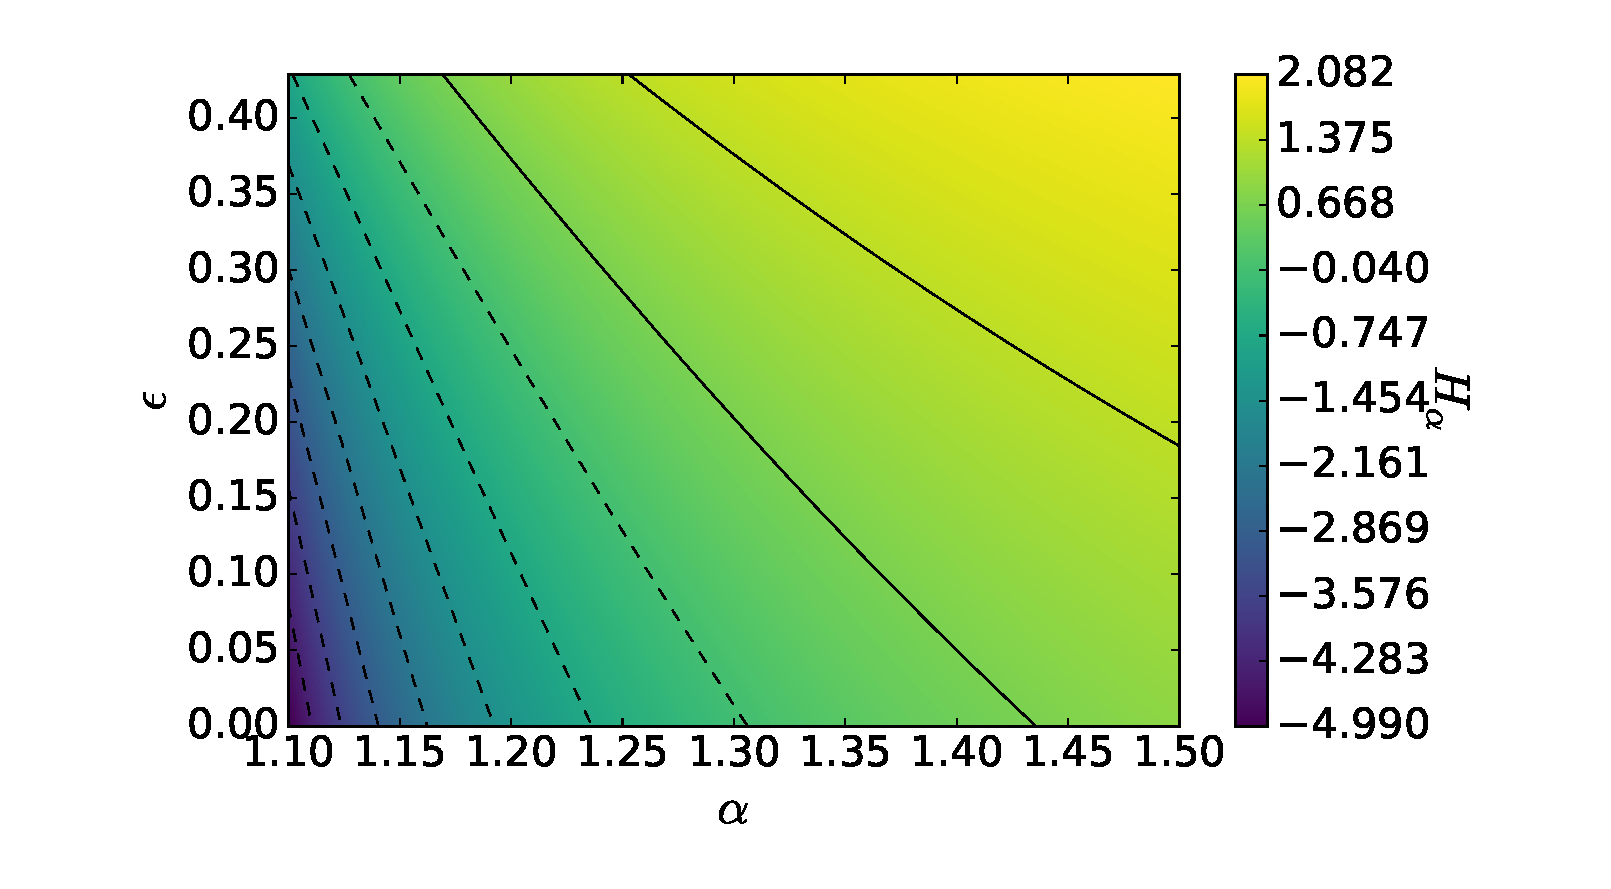
\includegraphics[scale=0.35]{figs/test/H_vs_eps_a.pdf}
    \caption{\ddd{[TO DO: Set $\epsilon = 0$ and determine region of $\alpha$ such that $H <0$.]} Here, the exponent is $\alpha =$ even$/$odd for $1.10 \leq \alpha \leq 1.50$. $H_\alpha$ is increasing in $\alpha$ and $\epsilon$ \nick{should be easy to show analytically}. First dashed contour from the right corresponds to $H_\alpha(\rho_{\rm{S}}(\epsilon)) = 0$. Specifically, $H_\alpha(\rho_{\rm{S}}(0)) = 0$ has a unique solution, which is the \nick{probably irrational - this seems problematic} solution of $3^\alpha - 2^{3-\alpha} = 1$.
    }
    \label{fig:lcs}
\end{figure}

We can prove additivity of $H_{\alpha}$ on quantum states.

\begin{lemma}\label{H_add}
	For any quantum states $\rho, \rho'$, we have
	\begin{equation}
		H_{\alpha}(\rho \otimes \rho') = H_{\alpha}(\rho) + H_{\alpha}(\rho'),
	\end{equation}
	where $\hspace{-1pt}\alpha\hspace{-1pt}$ is such that $\hspace{-1pt}H_\alpha(\sigma)\hspace{-2pt}$ is well-defined for all states $\sigma$.
\end{lemma}
\begin{proof}
	This can be seen directly by the multiplicative property of the Wigner distribution,
	\begin{align*}
		H_{\alpha}&(\rho \otimes \rho') = \frac{1}{1-\alpha}\log \sum_{\bmx,\bmx'} \left[W_{\rho}(\bmx)W_{\rho}(\bmx')\right]^{\alpha} \\
		&= \frac{1}{1-\alpha}\left( \log \sum_{\bmx}W_{\rho}(\bmx)^{\alpha} + \log \sum_{\bmx'}W_{\rho}(\bmx')^{\alpha} \right) \\
		&= H_{\alpha}(\rho) + H_{\alpha}(\rho').
	\end{align*}
\end{proof}

We then prove the following result connecting simple majorization to relative majorization.
\nick{move following lemma to section on relative majorization equivalent conditions}
\begin{lemma}
Let $\w\in \mathbb{R}^N, \w'\in \mathbb{R}^{N'}$ be quasi-distributions and $\r\in \mathbb{R}^N, \r'\in \mathbb{R}^{N'}$ probability distributions with positive rational entries given by $r_i = a_i/K$ and $r_i' = a_i'/K$ for positive integers $a_i, a_i'$ and $K = \sum_{i=1}^N a_i = \sum_{i=1}^{N'} a_i'$. 
Then,
\begin{equation}
(\w, \r) \succ (\w', \r') \mbox{ if and only if } \Gamma_{\bma} (\w) \succ \Gamma_{\bma'} (\w'),
\end{equation}
where the embedding map $\Gamma_{\bma} :\mathbb{R}^N \rightarrow \mathbb{R}^K$ is given by
\begin{equation}
	\Gamma_{\bma}(\x) := \bigoplus_{i=1}^N x_i \eta_{a_i},
\end{equation}
with $\eta_{a_i} = (1/a_i, 1/a_i, \dots, 1/a_i)$ the uniform distribution on $a_i$ elements.
\end{lemma}
\begin{proof}
	We first note that the map $\Gamma_{\bma}$ is stochastic and has a well-defined left-inverse $\Gamma^{-1}_{\bma'}: \mathbb{R}^K \rightarrow \mathbb{R}^N$ given by
\begin{equation}
	\Gamma^{-1}_{\bma}(\w) = \left( \sum_{i=1}^{a_1} w_i,  \sum_{i = a_1 +1}^{a_1 + a_2} \hspace{-5pt} w_i, \dots , \hspace{-15pt} \sum_{i=a_1 + \dots + a_{N-1}+1}^{K} \hspace{-10pt} w_i \right),
\end{equation}
that obeys $(\Gamma^{-1}_{\bma} \circ \Gamma_{\bma}) (\x) = \x$ for all $\x \in \mathbb{R}^N$. 

The claim is equivalent to the statement that there exists a \emph{bistochastic map} $B$ sending $\Gamma_{\bma}(\w)$ to $\Gamma_{\bma'}(\w')$ if and only if there exists a stochastic map $A$ sending $\w$ to $\w'$ and $\r$ to $\r'$.

Suppose there is a stochastic map $A$ such that $A\w=\w'$ and $A\r = \r'$. 
We define $B:\mathbb{R}^K \mapsto \mathbb{R}^K$ by $B := \Gamma_{\bma'} \circ A \circ \Gamma_{\bma}^{-1}$ so that it is stochastic as a composition of stochastic maps and it preserves the uniform distribution in $\mathbb{R}^A$, since
\begin{align}
	&B(1/K, 1/K, \dots, 1/K) = \big( \Gamma_{\bma'} \circ A \circ \Gamma_{\bma}^{-1} \big) \big( \Gamma_{\bma'}(\r) \big) = \nonumber\\
	&\Gamma_{\bma'} (\r') = (1/K, 1/K, \dots, 1/K),
\end{align}
therefore $B$ is bistochastic.
Finally, $B$ maps the embedded distributions as follows,
\begin{equation}
	B \Gamma_{\bma}(\w) = \big( \Gamma_{\bma'} \circ A \circ \Gamma_{\bma}^{-1} \big) \big( \Gamma_{\bma}(\w) \big) = \Gamma_{\bma'} (\w').
\end{equation}

Conversely, suppose a bistochastic map $B$ exists sending $\Gamma_{\bma}(\w)$ to $\Gamma_{\bma'}(\w')$. Again, define $A: \mathbb{R}^N \mapsto \mathbb{R}^{N'}$ by $A := \Gamma_{\bma'}^{-1} \circ B \circ \Gamma_{\bma}$ so that it is stochastic as a composition of stochastic maps and $A \w = \big( \Gamma_{\bma'}^{-1} \circ B \circ \Gamma_{\bma} \big) \w = \w'$, as well as $A \r = \r'$.
\end{proof}
We note that the vectors $\r, \r'$ with rational components form a dense subset of the positive probability distributions, so we can appeal to the fact that experiments have a finite resolution to ignore technical details regarding the completion to arbitrary real components.

\subsubsection{Unital fragment}

We now make use of known results from majorization theory to establish the Schur-concavity of $H_\alpha$ on Wigner quasi-distributions where $\alpha$ is such that $H_\alpha$ is well-defined. 
We first define the notion of \emph{Schur-convex and Schur-convave functions} on a subset $\D \subseteq \mathbb{R}^N$.

\begin{definition} 
A continuous, real-valued function $f$ defined on $\mathcal{Q} \subseteq \mathbb{R}^N$ is called Schur-convex on the domain $\mathcal{Q}$ if $\p \prec \q$ on $\mathcal{Q}$ implies that $f(\p) \le f(\q)$. A continuous function $f:\mathcal{Q} \rightarrow \mathbb{R}$ is called Schur-concave if $(-f)$ is Schur-convex.
\end{definition}
We can consider the set of all quasi-distributions, which form a hyper-plane and are given by
\begin{equation}
\mathcal{Q} = \left\{ \w \in \mathbb{R}^N: \sum_{i=1}^N w_i = 1 \right\}.
\end{equation}
For functions that are symmetric, namely $f(\p) = f(\Pi \p)$ for any component permutation $\Pi$, it suffices to restrict to the following region,
\begin{equation}
\mathcal{Q}^\downarrow = \{ \w \in \mathcal{Q} : w_1 \ge w_2 \ge \cdots \ge w_N\}.
\end{equation}

We now have the following theorem~\cite{cit:marshall} that provides a characterization of symmetric, Schur-convex and Schur-concave functions on quasi-distributions.
\begin{lemma}
Let $f$ be a real-valued continuous function defined on $\mathcal{Q}^\downarrow$ that is continuously differentiable on the interior of $\mathcal{Q}^\downarrow$. 
Then, $f$ is Schur-convex on $\mathcal{Q}^\downarrow$ if and only if $\partial_k f(\w)$ is decreasing in $k$ for all $\w \in \mathcal{Q}^\downarrow$, namely
\begin{equation}
\partial_1 f(\w) \ge \partial_2 f(\w) \ge \cdots \ge \partial_N f(\w),
\end{equation}
for all $\w$ in the interior of $\mathcal{Q}^\downarrow$.
\end{lemma}

We can use the above to prove that $H_\alpha$ is Schur-concave on quasi-distributions for particular values of $\alpha$.

\ddd{[TO-DO TIDY AND CHECK]}
\begin{theorem}\label{thm:HSchur}
	Let $\alpha = \frac{2a}{2b-1}$ for any positive integers $a,b$ with $a \geq b$.
	Then, $H_\alpha$ is Schur-concave, i.e. for quasi-distributions $\w, \w' \in \mathbb{R}^N$, we have $H_\alpha(\w) \leq H_\alpha(\w')$, whenever $\w \succ \w'$.
\end{theorem}
\begin{proof}
We have $\alpha = \frac{2a}{2b+1} \geq \frac{2b}{2b-1} > 1$ and $\alpha$ is a rational with even numerator and odd denominator, so $\sum_i x_i^\alpha > 0$ and $H_\alpha(\x)$ is well-defined for all quasi-distributions $\x$.

Given a fixed $\alpha$ for which $H_\alpha(\x)$ is well-defined, the function $H_\alpha$ is real-valued, smooth on the interior of $\mathcal{Q}^\downarrow$ and symmetric on any component permutation of $\x$.

Consider the partial derivatives
\begin{equation}
	\frac{\partial H_\alpha}{\partial w_i} = \frac{\alpha}{(\alpha-1)\sum_k{w_k^\alpha}}(-w_i^{\alpha-1}).
\end{equation}
We first note that for $\alpha$ in the given form, it is always true that
\begin{equation}
	\frac{\alpha}{(\alpha-1)\sum_k{w_k^\alpha}} > 0.
\end{equation}
We then show that for $\alpha$ in the given form, the function $f(w) = -w^{\alpha - 1}$ is non-increasing.
To this end, we first note that, for $\alpha > 1$, $f(w)$ has no discontinuities and we then obtain the first derivative
\begin{equation}
	f'(w) = -(\alpha - 1) w^{\alpha-2} = -(\alpha - 1)w^{\frac{2a-4b+2}{2b-1}} \leq 0,
\end{equation}
because $\alpha > 1$ and
\begin{equation}
	w^{\frac{2a-4b+2}{2b-1}} = \left(w^{2a-4b+2}\right)^{\frac{1}{2b-1}} = \left(w^{\frac{1}{2b-1}}\right)^{2(a-2b+1)} \geq 0,
\end{equation}
where each expression is well-defined because the rational exponent has odd denominator.

\nick{This step is the reason why $\alpha =$ odd$/$odd or $\alpha < 1$ do not work.

Example 1: if $\alpha =$ odd$/$odd, then $f(w)$ is not monotonous because the sign of $f'(w)$ would depend on the sign of $w$. 
In~\cref{tab:test}, this case fails when $w_i > 0 > -w_i > w_{i+1}$.

Example 2: if $\alpha =$ even$/$odd and $\alpha < 1$, then  $f(w)$ is not monotonous across $0$ because and in fact $\lim_{w\rightarrow 0^+} f(w) = -\infty$, while $\lim_{w\rightarrow 0^-} f(w) = +\infty$. 
In~\cref{tab:test}, this case fails when $w_i > 0 > w_{i+1}$.
}

Therefore, whenever $w_i \geq w_j$, we have that 
\begin{equation}
	-w_i^{\alpha-1} \leq -w_j^{\alpha-1},
\end{equation}
which leads to
\begin{equation}
	\frac{\partial H_\alpha}{\partial w_i} \leq \frac{\partial H_\alpha}{\partial w_j}.
\end{equation}
Therefore, $H_\alpha$ is Schur-concave and
\begin{equation}
	H_\alpha(\w) \leq H_\alpha(\w'),
\end{equation}
for any quasi-distributions $\w, \w'$ that obey $\w \succ \w'$.


\begin{table}[h]
  \def\arraystretch{1.5}
  \centering
  \begin{tabular}{c|c|c|c||c|c}
    $w_i$ & $w_{i+1}$ & $\alpha$ & $\frac{w_i^{\alpha-1}}{\alpha-1} \geq \frac{w_{i+1}^{\alpha-1}}{\alpha-1}$ & $\alpha$ & $\frac{w_i^{\alpha-1}}{\alpha-1} \geq \frac{w_{i+1}^{\alpha-1}}{\alpha-1}$ \\[0.5ex]\hline
    $2$ & $1.5$  & $3$ & $2 > 1.125$ T & $1/3$ & $-0.94 > -1.14$ T \\
    $2$ & $-1.5$ & $3$ & $2 > 1.125$ T & $1/3$ & $-0.94 > -1.14$ T \\
    $2$ & $-2.5$ & $3$ & $2 < 3.125$ F & $1/3$ & $-0.94 < -0.81$ F \\[0.5ex]\hline
    $2/3$ & $1/3$  & $3$ & $0.22 > 0.06$ T & $1/3$ & $-1.97 > -3.12$ T \\
    $2/3$ & $-1/3$ & $3$ & $0.22 > 0.06$ T & $1/3$ & $-1.97 > -3.12$ T \\
    $2/3$ & $-4/3$ & $3$ & $0.22 < 0.89$ F & $1/3$ & $-1.97 < -1.24$ F \\[0.5ex]\hline
    $2$ & $1.5$  & $4$ & $2.67 > 1.125$ T & $2/3$ & $-2.38 > -2.62$ T \\
    $2$ & $-1.5$ & $4$ & $2.66 > -1.125$ T & $2/3$ & $-2.38 > 2.62$ F \\
    $2$ & $-2.5$ & $4$ & $2.66 > 5.21$ T & $2/3$ & $-2.38 > 2.21$ F \\
    $-2$ & $-2.5$ & $4$ & $-2.66 > -5.21$ T & $2/3$ & $2.38 > 2.21$ T \\[0.5ex]\hline
    $2/3$ & $1/3$  & $4$ & $0.10 > 0.01$ T & $2/3$ & $-3.43 > -4.33$ T \\
    $2/3$ & $-1/3$ & $4$ & $0.10 > -0.01$ T & $2/3$ & $-3.43 > 4.33$ F \\
    $2/3$ & $-4/3$ & $4$ & $0.10 > -0.79$ T & $2/3$ & $-3.43 > 2.73$ F \\
    $-1/3$ & $-2/3$ & $4$ & $-0.01 > -0.10$ T & $2/3$ & $4.33 > 3.43$ T \\
    $-1/3$ & $-4/3$ & $4$ & $-0.01 > -0.79$ T & $2/3$ & $4.33 > 2.73$ T
  \end{tabular}
  \caption{\nick{NUMERICS ON SCHUR-OSTROWSKI CONDITION} The case $\alpha=$ even$/$odd and $\alpha > 1$ works for any combination of $w_i, w_{i+1}$ with $w_i > w_{i+1}$. 
  All other cases do not work.}
  \label{tab:test}
\end{table}

\end{proof}
The set $F := \{2a/(2b-1): a,b \in \mathbb{N} \text{ and } a \geq b\}$ is dense in the rationals $\mathbb{Q}_{>1}$, which in turn are dense in the reals $\mathbb{R}_{>1}$, as any rational $c/d$ with $c>d$ can be approximated by a sequence $f_n := c2^n / (d2^n+1)$ with every element $f_n$ in the set $F$. \nick{can turn into lemma}


We can now derive the following entropic bounds on magic state transformations.
\begin{theorem}
	Consider a general magic state distillation process $\rho^{\otimes n} \rightarrow \rho'^{\otimes n'}$	in the unital fragment.
	We have the following family of upper bounds on the distillation rate $R := n'/n$,
	\begin{equation}
		R \leq \frac{H_\alpha \left( \id/3 \right) - H_\alpha \left( \rho \right)}{H_\alpha \left( \id/3 \right) - H_\alpha \left( \rho') \right)} = \frac{D_{\alpha}(\rho||\id/3)}{D_{\alpha}(\rho'||\id/3)},
	\end{equation}
	where $\alpha = \frac{2a}{2b-1}$ for any positive integers $a,b$ with $a \geq b$.
\end{theorem}
\begin{proof}
	For the given form of $\alpha$, $H_\alpha(\sigma)$ is well-defined adn Schur-concave for all quantum states $\sigma$.
	
	We first regularise the number of output copies in the state distillation by tensoring in $(n-n')$ copies of the (free) maximally mixed state $\id/3$, so that we instead consider the process
\begin{equation}
	\rho^{\otimes n} \rightarrow \rho'^{\otimes n'} \otimes \left( \frac{1}{3}\id \right)^{\otimes (n - n')}.
\end{equation}
Since we have that $W_{\rho^{\otimes n}}(\bmx) \succ_{\id/3} W_{\rho'^{\otimes n'}}(\bmx)$, by Schur-concativity of $H_\alpha$ we obtain
\begin{equation}
	H_\alpha \left( \rho^{\otimes n} \right) \leq H_\alpha \left( \rho'^{\otimes n'} \otimes \left( \frac{1}{3}\id \right)^{\otimes (n - n')} \right).
\end{equation}
By additivity of $H_\alpha$, we can rewrite the inequality as
\begin{equation}
	n H_\alpha \left( \rho \right) \leq n' H_\alpha \left( \rho' \right) + (n - n') H_\alpha \left( \id/3 \right).
\end{equation}
Now, $H_\alpha \left( \id/3 \right)$ is the maximum value of $H_\alpha(\rho)$ for unital processes because every state $\rho$ majorizes $\id/3$, so we can finally re-arrange the inequality to
\begin{equation}
	\frac{n'}{n} \leq \frac{H_\alpha \left( \id/3 \right) - H_\alpha \left( \rho \right)}{H_\alpha \left( \id/3 \right) - H_\alpha \left( \rho' \right)}.
\end{equation}
\end{proof}

\subsubsection{Extention to general relative majorization}

Therefore if we have a Schur-Concave function $f(\x)$ for majorization of quasi-distributions then we can define a monotonic function for relative majorization via composition with $\Gamma_{\mathbf{a}}$ and its inverse.
This should provide relative majorization monotones from which we can obtain distillation bounds, such as
\begin{equation}
R \le \frac{F_\alpha(\tau) - F_\alpha (\rho)}{F_\alpha(\tau') - F_\alpha (\rho')}.
\end{equation}
\ddd{[To be checked...transition from entropies to free energies less obvious from this route...needs reflection]}

This is probably all we need to show:
\begin{equation}
H_\alpha(\Gamma_{\mathbf{a}}(\p)) = D_\alpha(\p ||\r),
\end{equation}
where we define the Renyi relative entropy
\begin{equation}
D_\alpha (\p || \r) := \frac{1}{\alpha -1} \log \sum_i p_i^\alpha q_i^{1-\alpha}.
\end{equation}
This probably follows from the details of how the $\Gamma_{\mathbf{a}}$ relates to $\r$. Needs expanding carefully.

\begin{theorem}
	Consider a general magic state distillation process that converts magic state $\rho^{\otimes n} \longrightarrow \rho'^{\otimes n'}$ as well as equilibrium state $\tau^{\otimes n} \longrightarrow \tau'^{\otimes n'}$, where we assume that $W_{\tau^{\otimes n}}(\bmx) = a_{\bmx}/K$ and $W_{\tau'^{\otimes n'}}(\bmx) = a_{\bmx}/K$ for positive integers $a_{\bmx}, a_{\bmx}'$ and $K = \sum_{\bmx} a_{\bmx} = \sum_{\bmx} a_{\bmx}'$.  \nick{It may be more convenient to consider $W_{\tau}(\bmx') = a_{\bmx'}/K$, so that $K$ ends up raised to the power of $n$}
	
	We have the following family of upper bounds on the distillation rate $R := n'/n$,
	\begin{equation}
		R \leq \text{\nick{BOUND}},
	\end{equation}
	where $\alpha = \frac{2a}{2b-1}$ for any positive integers $a,b$ with $a \geq b$.
\end{theorem}
\begin{proof}
	For the sake of clarity, we write $\rho_n \coloneqq \rho_S(\epsilon)^{\otimes n}$, $\rho'_{n'} \coloneqq \rho_S(\epsilon')^{\otimes n'}$, $\tau_n \coloneqq \tau^{\otimes n}$ and $\tau'_{n'} \coloneqq \tau'^{\otimes n'}$.
	
	We have that 
\begin{equation}	
	\Big(W_{\rho_n}(\bmx), W_{\tau_n}(\bmx')\Big) \succ \Big(W_{\rho'_{n'}}(\bmx), W_{\tau'_{n'}}(\bmx')\Big)
\end{equation}	
or equivalently $\Gamma_{\bma}(W_{\rho_n}(\bmx)) \succ \Gamma_{\bma'}(W_{\rho'_{n'}}(\bmx))$ for all $\bmx$, where
\begin{align}
	\Gamma_{\bma}(W_{\rho_n}) &= \bigoplus_{\bmx} W_{\rho_n}(\bmx) \left(\frac{1}{KW_{\tau_n}(\bmx)}, \dots, \frac{1}{KW_{\tau_n}(\bmx)} \right)\nonumber\\
	&= \frac{1}{K}\bigoplus_{\bmx} \Big( W_{\rho_n|\tau_n}(\bmx), \dots, W_{\rho_n|\tau_n}(\bmx) \Big)
\end{align}
and similarly for $\Gamma_{\bma'}(W_{\rho'_{n'}})$.
Therefore,
\begin{align}
	&H_{\alpha}(\Gamma_{\bma}(W_{\rho_n})) = \frac{1}{1-\alpha} \log_2 \left( \frac{d^{2n}}{K^\alpha} \sum_{\bmx} \big[ W_{\rho_n|\tau_n}(\bmx) \big]^\alpha \right) = \nonumber\\
	&\frac{1}{1-\alpha} \log_2 \left( \frac{d^{2n}}{K^\alpha} \sum_{\bmx_1, \dots, \bmx_n} \big[ W_{\rho|\tau}(\bmx_1) \dots W_{\rho|\tau}(\bmx_n) \big]^\alpha \right)
\end{align}
while
\begin{equation}
	D(\rho||\tau) = \frac{1}{\alpha-1} \log_2 \sum_{\bmx} \frac{W_{\rho}(\bmx)^\alpha}{W_{\tau}(\bmx)^{\alpha-1}}.
\end{equation}
\nick{correct mistakes, bridge gaps}
\end{proof}


\subsection{Dropping pre/post-processing of the magic states}
\label{app:cliff_processing}

If we drop the freedom to transform the magic states via Clifford unitaries, then the final expression for the bounds change and become a little more complex, since the largest component in the rescaled distribution depends on a number of factors. We illustrate this by the following result.

\begin{theorem}\label{thm:no-processing}
	Consider a magic distillation protocol on qutrits that transforms
\begin{equation*}
	\rho_S(\epsilon)^{\otimes n} \longrightarrow \E(\rho_S(\epsilon)^{\otimes n})=\rho_S(\epsilon')^{\otimes m} 
\end{equation*}
with $n, m \gg 1$.

Let each qutrit have a Hamiltonian $H$ with energies $E_0, E_1, E_2$ and stabilizer eigenstates, and define $E_{\rm max} = \max\{E_0, E_1, E_2\}$ and \nick{$E_s$ as the eigenvalue of the Hamiltonian eigenstate whose Wigner distribution overlaps the negative component of $\rho_S(\epsilon)$ in the phase space.}
Let $T =(k\beta)^{-1}$ be any finite temperature and assume that in the thermodynamic limit ($n,m \gg 1$), the protocol applied to the equilibrium state $\tau^{\otimes n} = (e^{-\beta H}/\Z)^{\otimes n}$ maps $\tau^{\otimes n} \longrightarrow \tau^{\prime \otimes m}$, where we express state $\tau'$ as $\tau' = e^{-\beta H'}/\Z'$ for some Hermitian $H'$.

Define $\beta_\star = (k T_\star)^{-1}$ through the relation
\begin{equation}
	E_{\rm max} - E_s \eqqcolon kT_\star \ln 2,
\end{equation}
and define a threshold error,
\begin{equation}\label{eq:threshold}
	\epsilon_{\star}(\beta) \coloneqq 
	\begin{cases}
		3 - \dfrac{9}{4-2^{\beta/\beta_\star - 1}}, &\text{ for } \beta \leq \beta_\star \\
		0, &\text{ for } \beta > \beta_\star.
	\end{cases}
\end{equation}
Then, the distillation rate $R = m/n$ of the magic protocol is bounded as:
\begin{equation}
	R \leq
	\begin{cases}
		\dfrac{\ln{\big( 1-\frac{4}{3}\epsilon \big)} + \beta (E_s - F)}{\ln{\big( 1-\frac{4}{3}\epsilon' \big)} + \beta (E'_s - F')},\ &\epsilon \leq \epsilon_\star, \epsilon' \leq \epsilon'_\star, \vspace{10pt}\\
		\dfrac{\ln{\big( 1-\frac{4}{3}\epsilon \big)} + \beta (E_s - F)}{\ln{\big( \frac{1}{2}-\frac{1}{6}\epsilon' \big)} + \beta (E'_{\rm{max}} - F')},\ &\epsilon \leq \epsilon_\star, \epsilon' > \epsilon'_\star, \vspace{10pt}\\
		\dfrac{\ln{\big( \frac{1}{2}-\frac{1}{6}\epsilon \big)} + \beta (E_{\rm{max}} - F)}{\ln{\big( 1-\frac{4}{3}\epsilon' \big)} + \beta (E'_s - F')},\ &\epsilon > \epsilon_\star, \epsilon' \leq \epsilon'_\star, \vspace{10pt}\\
		\dfrac{\ln{\big( \frac{1}{2}-\frac{1}{6}\epsilon \big)} + \beta (E_{\rm{max}} - F)}{\ln{\big( \frac{1}{2}-\frac{1}{6}\epsilon' \big)} + \beta (E'_{\rm{max}} - F')},\ &\epsilon > \epsilon_\star, \epsilon' > \epsilon'_\star,
	\end{cases}
\end{equation}
where $F$ is the free energy of state $\tau$ and all primed quantities are similarly defined for the ouptut system.
\end{theorem}
\begin{proof}
The proof proceeds in the same manner as in~\cref{thm:free-energy-bound-proof} up to the point where we need to evaluate $W_{\rho_n |\tau_n} (\x)$ and $W_{\rho_n}(\x)$ explicitly, beyond which we do not have the freedom of additional Clifford processing.

\nick{Explain why this is not Clifford processing, ensure overlap with negativity is the one suggested}
The equilibrium state at inverse temperature $\beta$ on a single qutrit is given by $\tau = e^{-\beta H} / \Z$. Moreover we have that $\tau$ is a full-rank stabilizer state, where $\beta \geq 0$ and $H = E_0 |\varphi_0\>\<\varphi_0| + E_1 |\varphi_1\>\<\varphi_1| + E_2 |\varphi_2\>\<\varphi_2|$ is an eigendecomposition of $H$.
The state $\tau$ can now be written as 
\begin{equation}
	\tau = \frac{e^{-\beta E_0}}{\Z} |\varphi_0\>\<\varphi_0| + \frac{e^{-\beta E_1}}{\Z} |\varphi_1\>\<\varphi_1| + \frac{e^{-\beta E_2}}{\Z} |\varphi_2\>\<\varphi_2|,
\end{equation}
where the eigenstates $\{\ket{\varphi_k}\<\varphi_k|\}$ are pure, orthonormal stabiliser states, which can be represented in terms of generalized Paulis. We are free to redefine the computational basis so it coincides with the basis of $H$. Abstractly, let $C$ be the unitary transforming each $|\varphi_k\>\<\varphi_k|$ to $|k\>\<k|$. Since the Clifford group is the normalizer of the Heisenberg-Weyl group, $C$ is a Clifford unitary. Therefore, $C$ maps $\tau$ to another stabilizer state that is diagonal in the computational basis, and we can assume without loss of generality that $\tau$ is diagonal in $\{|0\>,|1\>, |2\>\}$. However, this re-definition of the computational basis means that the location of the negative Wigner component $-v(\epsilon)$ of the Strange state will be permuted on the discrete phase space. We denote by $E_s$ the eigenvalue of $H$ where the associated eigenvector has Wigner distribution overlapping the negative component of the magic state $C\rho_S(\epsilon)C^\dagger$.  This is unique, since the eigenstates form an orthonormal basis.

The Wigner distribution of state $\tau$ is then given by
\begin{align}
	\W[\bmx]{\tau} &= \sum\limits_{k=0}^2 \frac{e^{-\beta E_k}}{\Z}W_{|k\>\<k|}(x, p) \nonumber\\
	&= \sum\limits_{k=0}^2 \frac{e^{-\beta E_k}}{\Z} \delta_{x, k} = \frac{e^{-\beta E_x}}{3\Z},
\end{align}
where $x$ labels one of the three vertical lines in the phase space.
The rescaled Wigner distribution $W_{\rho|\tau}(\x)$ can now be computed. It has $9$ components, but these come with multiplicities. In total, there are four distinct values on the phase space, as illustrated in~\cref{fig:pd_split}.
\begin{figure}[h]
    \centering
    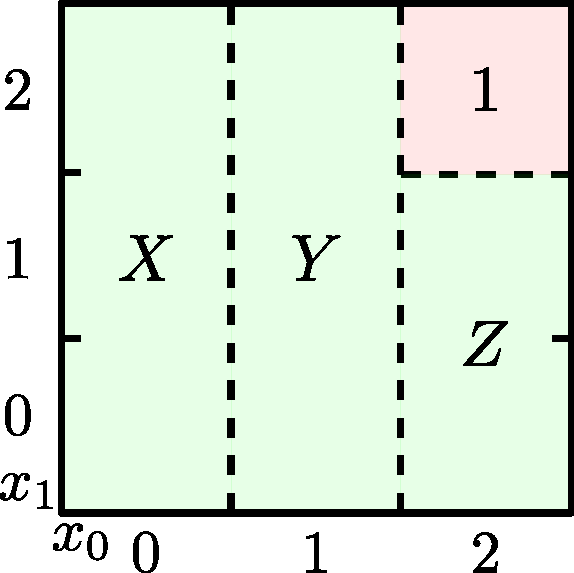
\includegraphics[scale=0.45]{figs/pd_split_thermal.pdf}
    \caption{\textbf{Qutrit phase space regions for $W_{\rho | \tau}(\x)$.}
    Here, the negative component of the magic state overlaps the Wigner distribution of $|0\>$. The rescaled distribution attains a single value in each of the four regions, proportional to the value depicted in the region, see~\cref{eq:bmw_rescaled}.
    }
    \label{fig:pd_split}
\end{figure}

We denote by $\w(\rho), \w(\rho|\tau)$ the unique values occurring in $W_\rho(\x), W_{\rho|\tau}(\x)$ respectively and $\bmm$ the vector of associated multiplicities of each value in $W_\rho(\x)$. The component values and multiplicities of the relevant distributions in the four distinct regions are given by
\begin{align}
	\w(\rho) &\coloneqq (-v, u, u, u), \\
		\bmm &\coloneqq (1,2,3,3), \\
	\w(\tau) &\coloneqq \frac{1}{3\Z} \left( e^{-\beta E_0}, e^{-\beta E_0}, e^{-\beta E_1}, e^{-\beta E_2} \right), \\
	\w(\rho_{\rm{S}} | \tau) &\coloneqq 3\Z \left( -v e^{\beta E_0}, u e^{\beta E_0}, u e^{\beta E_1}, u e^{\beta E_2} \right). \label{eq:bmw_rescaled}
\end{align}

Using this notation, the values and multiplicities of the $n$--copy distribution $\bmw(\rho_n |\tau_n)$ are computed in~\cref{lem:ncopycomponents}. The values are given by 
\begin{align}\label{eq:ncopy_w_rescaled}
	[\w(\rho_n | \tau_n)]_{ijk} &= (3\Z)^{n} (-v)^{n-\alpha} u^{\alpha} e^{\beta (n-\alpha)E_s} e^{\beta ( i E_0 + j E_1 + k E_2 )},
\end{align}
where the indices $i,j,k$ are non-negative integers that obey the constraint $\alpha \coloneqq i+j+k \leq n$.
The multiplicity of this above value is $m_{ijk}$ with
\begin{equation}
	m_{ijk} = \frac{n!}{i!j!k!(n-\alpha)!} 2^i 3^j 3^k.
\end{equation}
The associated components of $\w(\rho_n)$ are given by
\begin{align}
	[\w(\rho_n)]_{ijk} &= (-v)^{n-\alpha} u^{\alpha}, \label{eq:ncopy_wrho}\\
	[\w(\tau)]_{ijk} &= (3\Z)^{-n} e^{-\beta (n-\alpha)E_s} e^{-\beta ( i E_0 + j E_1 + k E_2 )}. \label{eq:ncopy_wsigma}
\end{align}

In order to construct the $n$--copy Lorenz curve $L_{\rho_n|\tau_n}(x)$ we need to order the components of the distribution, $w(\rho_{\rm{S}} | \tau)_{ijk}$ in decreasing order, and identify the sequence of indices that give us $W_{\rho_n}(\pi(\x))$.

However, it again suffices to use only the constraint from the first elbow $(x_0, L_0)$ of $L_{\rho_n|\tau_n}(\x)$. We therefore compute the largest component 
\begin{equation}
	w_{\rm max} \coloneqq \max_{i,j,k} [\w(\rho_n | \tau_n)]_{ijk},
\end{equation}
and determine the indices at which this occurs.
Putting in the values we obtain
\begin{align}
	&(3\Z)^{-n}w_{\rm max} = \nonumber\\
	&\max\limits_{i,j,k}\Big\{ (-v)^{n-\alpha} u^{\alpha} e^{\beta (n-\alpha)E_s} e^{\beta ( i E_0 + j E_1 + k E_2 )} \Big\}, \label{eq:max_slope}
\end{align}
where $0 \leq i,j,k \leq n$ and $\alpha \coloneqq i+j+k \leq n$.
Now for $0 \leq \epsilon \leq 3/7$, we have $v \geq u$. Since we assume that $n$ is even, we need the sum $\alpha = i+j+k$ to be even too, so that the expression is positive. 

Given an even value for $\alpha$, the term $v^{n-\alpha} u^{\alpha} e^{-\beta (n-\alpha)E_s}$ is fixed, so the expression is maximised by setting the coefficient of the highest energy $E_{\rm{max}}$ equal to $\alpha$.
Hence, we have
\begin{align}
	&w_{\rm max} = \nonumber\\
	&(3\Z)^{n} v^n e^{n\beta E_s}\max\limits_{\substack{\alpha = 0,2, \\ \dots,n-2,n}}{\Big\{ \left( \frac{u}{v} e^{\beta (E_{\rm{max}} - E_s)} \right)^{\alpha} \Big\}}.
\end{align}
If the expression $\frac{u(\epsilon)}{v(\epsilon)} e^{\beta (E_{\rm{max}} - E_s)}$ is less than $1$ then the maximum occurs at $\alpha=0$, otherwise it occurs at $\alpha = n$. For a fixed state $\tau$, this transition is determined by the value of the depolarising error parameter $\epsilon$ of the noisy magic state. The transition occurs at $\epsilon = \epsilon_\star$ where
\begin{equation}\label{eq:noise_transition}
	\frac{u(\epsilon_\star)}{v(\epsilon_\star)} e^{\beta (E_{\rm{max}} - E_s)} = \frac{3-\epsilon_\star}{6-8\epsilon_\star} e^{\beta (E_{\rm{max}} - E_s)} = 1.
\end{equation}
If $E_{\rm{max}} = E_s$, namely if the state negativity lies in the same phase space region as the highest energy, this threshold is constant in temperature and given by $\epsilon_{\star} = 3/7$. However, the condition that $\epsilon_\star \ge 0$ also implies a constraint on the effective temperature of the stabilizer state. Specifically, there is a threshold temperature value $\beta_\star$ given by
\begin{equation}
	\beta_{\star} \coloneqq \frac{1}{E_{\rm{max}} - E_s} \ln2,
\end{equation}
such that for the regime $0 \leq \beta \leq \beta_\star$ a threshold error $\epsilon_\star$ exists, and for $\beta > \beta_\star$ no such transition exists, so we choose $\epsilon_\star = 0$. 
Therefore, the transition value for the noise is given by
\begin{equation}
	\epsilon_{\star}(\beta) \coloneqq 
	\begin{cases}
		3 - \dfrac{9}{4-2^{\beta/\beta_\star - 1}}, &\text{ for } \beta \leq \beta_\star \\
		0, &\text{ for } \beta > \beta_\star.
	\end{cases}
\end{equation}
The quantity $w(\rho_{\rm{S}} | \sigma)_{\rm{max}}$ is now given by
\begin{equation*}
w_{\rm max} =
	\begin{cases}
		(3\Z)^{n} v^n e^{n\beta E_s}, &\mbox{if }\epsilon \leq \epsilon_{\star},\ \hspace{3pt}\rm{(C1)}\\
		(3\Z)^{n} u^n e^{n\beta E_{\rm{max}}}, &\mbox{if }\epsilon > \epsilon_{\star}.\ \hspace{5pt}\rm{(C2)} 
	\end{cases}
\end{equation*}
Case $\rm{(C1)}$ corresponds to $(i,j,k) = (0,0,0)$, so the multiplicity is $m_{000} = 1$, while
Case $\rm{(C2)}$ corresponds to
\begin{equation}
	(i,j,k) = 
	\begin{cases}
	(0,n,0), &\text{if } E_{\rm{max}} = E_1, \\
	(0,0,n), &\text{if } E_{\rm{max}} = E_2,
	\end{cases}
\end{equation}
so the multiplicity in both cases is $3^n$.

Using that $F = -\beta^{-1} \log \Z$, the first elbow coordinates in the two cases are now given by
\begin{equation}\label{eq:first_elb_coords}
	(x_0, L_0) =
	\begin{cases}
		\left(\frac{1}{3^n} e^{-n\beta (E_s - F)}, v^n \right), &\epsilon \leq \epsilon_\star \vspace{10pt}\\
		\left( e^{-n\beta (E_{\rm{max}}-F)}, (3u)^n \right). &\epsilon > \epsilon_\star
	\end{cases}
\end{equation}

Similarly, considering the output magic state with respect to state $\sigma'$, the image of equilibrium state $\sigma$ under the magic protocol, we get output Lorenz curve coordinates,
\begin{equation}\label{eq:transformed_first_elb_coords}
	(x'_0, L'_0) =
	\begin{cases}
		\left(\frac{1}{3^{n'}} e^{-n\beta (E'_s - F')}, v(\epsilon')^{n'} \right), &\epsilon' \leq \epsilon'_\star \vspace{10pt}\\
		\left( e^{-n'\beta (E'_{\rm{max}}\hspace{-2.5pt}-F')}, (3u(\epsilon'))^{n'} \right), &\epsilon' > \epsilon'_\star
	\end{cases}
\end{equation}
There are four combinations of coordinates, depending on the noise parameters $\epsilon, \epsilon'$ for the input and output states.
In each of these combinations, we simply use the first elbow constraint, as described in~\cref{prop:first_elb}, and manipulate the coordinates as in the proof of~\cref{thm:free-energy}, leading to the bounds in the statement of the theorem.
\end{proof}































\end{document}